\chapter[Practical Considerations]{Practical Considerations in
Nonlinear Regression}

\index{practical considerations!in nonlinear regression}
\index{nonlinear!regression, practical considerations"}
\prologue{Rationally, let it be said in a whisper, experience is
certainly worth more than theory.}{Amerigo Vespucci}

Nonlinear estimation, like all data analysis procedures, involves
many practical considerations.
In this chapter, we discuss some
techniques which help ensure a successful nonlinear analysis.
The topics include model specification,
preliminary analysis,
determination of starting values,
transformations of parameters and variables,
other iteration schemes,
convergence,
assessment of fit and modification of models,
correlated residuals,
accumulated data,
comparison of models,
parameters as functions of other variables,
and
presentation of results.
A case study in which we illustrate many of the techniques presented
in this chapter is given in Section 3.13.
The important practical problem of designing experiments for nonlinear
models is discussed in the final section.
\section{Model Specification}
\index{practical considerations!model specification}
\index{model!specification in nonlinear regression}

An important step in any nonlinear analysis is specification of
the model, which includes specifying both the expectation function and the
characteristics of the disturbance.
\subsection{The Expectation Function}

Ideally, physical, biological, chemical, or other theoretical
considerations will lead to a \emph{mechanistic} model for the
expectation function.
The analyst's job is then to find the simplest form of the
model and the parameter estimates which provide an adequate fit of
the model to the data, subject to the assumptions about the
disturbance.
Note that it is not necessary for the expectation function to be
stated as an explicit function of the parameters and the control
variables.
In Chapter 5 we discuss an important class of models, known as
compartment models, in which the expected response is given by
the solution to a set of linear differential equations.
Special techniques, developed in that chapter, can be used to
avoid solving explicitly for the expectation function in terms of
the parameters and independent variables.

In other situations, the expectation function may be the solution to a
nonlinear differential equation or an
\index{differential equation!specification of nonlinear model}
integral equation which has no analytic solution.
Then the value of the expectation function must be determined
numerically for any given parameter values for a regular
nonlinear least squares program to be used.
In such situations, numerical parameter derivatives or a
derivative-free optimization procedure will often have to be used
to calculate the least squares estimates.
However, as discussed in \citeasnoun{cara:stew:1985}, when an expectation function
%\glossary{ Caracotsios, M.}
%\glossary{ Stewart, W.E.}
is obtained from the solution to a set of ordinary differential
equations, the parameter derivatives of the expectation function
can be determined from the sensitivity functions for the
system of differential equations.
These functions are evaluated numerically at the same time
as the solution of the differential equations is evaluated.

\begin{example}\label{pin:nonlin}

The decomposition of $\alpha$-pinene was investigated by
\nocite{fugu:hawk:1945,fugu:hawk:1947}
Fuguitt and Hawkins (1945, 1947), who reported
%\glossary{ Fuguitt, R.E.}
%\glossary{ Hawkins, J.E.}
the concentrations of five reactants as a function of time,
at a series of reaction temperatures.
In Appendix A, Section~\ref{atbl:pin}, we present the data for the run at
189.5$^\circ$C.

We discuss these data in Chapters 4 and 5 and fit a model
which is specified by a set of linear differential equations.
As discussed in Chapter 5, the parameters in such models can be
estimated very easily, due to the ease with which they can be specified
and the ease with which the responses and the derivatives with respect
to the parameters can be evaluated.
As will be also shown in Chapter 5, however, the linear differential
equation model does not provide an adequate fit to the $\alpha$-pinene
data.

\citeasnoun{stew:soer:1981} analyzed the complete data set
%\glossary{ Stewart, W.E.}
%\glossary{ Soerensen, J.P.}
reported by \nocite{fugu:hawk:1945,fugu:hawk:1947}
Fuguitt and Hawkins (1945, 1947), and
%\glossary{ Fuguitt, R.E.}
%\glossary{ Hawkins, J.E.}
proposed a model consisting of a set of five nonlinear differential
equations
  \begin{eqnarray*}
    \frac{df_1}{dt}&=&-( \theta_1+\theta_2) f_1 -2 \theta_3 f_1^2\\
    \frac{df_2}{dt}&=&- \theta_4 f_2 + \theta_5 f_4\\
    \frac{df_3}{dt}& =& \theta_1 f_1\\
    \frac{df_4}{dt}&=&\theta_2 f_1 + \theta_4 f_2 -\theta_5 f_4 -2
    \theta_6 f_4^2 +2 \theta_7 f_5\\
    \frac{df_5}{dt}&=& \theta_8 f_1^2 +\theta_6 f_4^2-\theta_7 f_5
  \end{eqnarray*}
where $f_i ,i=1 ,\ldots,5$, represent the theoretical responses
at time $t$.

There is no analytic solution to this set of differential
equations, and so we must use numerical procedures.
For given values of
$\btheta=( \theta_1 ,\ldots,\theta_8 ) \trans$,
the differential equations would be integrated numerically using,
say, a Runge--Kutta integration routine \cite{cont:debo:1980}.
%\glossary{ Conte, S.D.}
%\glossary{ deBoor, C.}
The numerical estimates of the responses, ${\bf f} ( t )$, and the
observed responses $\by ( t )$,
at the observation times, could then be used to
calculate residuals from which an appropriate estimation criterion
can be evaluated.

We discuss the choice of estimation criterion for multiresponse data
in Chapter 4.
Methods for obtaining derivatives of the response functions at
the observation times by means of the
``sensitivity functions''
      \begin{displaymath}
        \frac{\partial f_i(t)}{\partial\theta_p}\quad
        i=1,\ldots,5\quad p = 1 ,\ldots, P 
      \end{displaymath}
are given in \citeasnoun{cara:stew:1985}.
%\glossary{ Caracotsios, M.}
%\glossary{ Stewart, W.E.}
The derivative matrix $\bV$ can then be calculated from the
sensitivity functions.
\end{example}

In other situations, a mechanistic model may not be advanced by
the researcher, in which case the statistician will be called
upon to suggest an equation.
One approach is to ask the researcher to search through the
literature to see if models have been proposed.
If not, the statistician and the researcher can apply their
modeling skills and develop a plausible mechanistic model.
Failing this, the statistician must formulate a model which has
the same sort of behavior as the data.
If the data rise monotonically to an asymptote, perhaps a
Michaelis--Menten, exponential rise, or logistic model might be
appropriate.
If the data peak and then decay towards zero, perhaps a
double exponential, a Michaelis--Menten model with a quadratic
term in the denominator, or a gamma function would be suitable.

Finally, if there are several sets of data, it may be possible to use
the self-modeling approach of \citeasnoun{lawt:sylv:magg:1972}.
%\glossary{ Lawton, W.H.}
%\glossary{ Sylvestre, A.}
%\glossary{ Maggio, M.S.}
This approach has been used in modeling spirometer curves
which give the volume of air expelled
from the lungs as a function of time for a number of subjects,
and in modeling the
creatine phosphokinase serum levels in patients suffering
myocardial infarctions \cite{arms:watt:hami:chio:park:1979}.
%\glossary{ Armstrong, P.W.}
%\glossary{ Watts, D.G.}
%\glossary{ Hamilton, D.C.}
%\glossary{ Chiong, M.A.}
%\glossary{ Parker, J.O.}

\subsection{The Disturbance Term}
\index{practical considerations!disturbance}
\index{disturbance!practical considerations}

All nonlinear estimation programs are based on specific
assumptions about the disturbance term, usually that the
disturbance is additive and normally distributed with zero mean,
constant variance, and independence between cases (see Section
1.3).
Checking assumptions on the disturbance term is considerably
easier and more sensitive
if the data include replications at some or all of the design
points.
It is helpful if the experimental runs have been randomized,
although many nonlinear experiments involve sequential
measurements of the response, so that randomization may not be
feasible.

At the initial stage, it is generally possible to check only one
of the assumptions on the disturbance, namely constancy of variance.
\index{variance!constant}
If there are replications, one can simply plot the data and look
\index{replication}
to see if the spread of the data tends to systematically increase
or decrease with respect to any of the predictor
variables.
Alternatively, one can use an analysis of variance program to
obtain averages and estimated variances and standard deviations for the
replicated responses and then plot the variances or standard deviations
versus the average, again looking for any
systematic relationship, as discussed in Section 1.3.
If none is apparent, then it may be tentatively assumed that the
variance is constant and the analysis can proceed;  if there is a
relationship, then oftentimes a simple power transformation such
as square root, logarithm, or inverse will stabilize the variance.
Even without replications, some visual indication of constancy of
variance can be gained from a data plot but this is
not as definitive as when replications are available.

Note that transforming the data also involves transforming the
expectation function.
Thus, if there is a well-justified expectation function for the
response but the data should be transformed to induce constant
variance, then the same transformation should be applied to the expectation
function to preserve the fundamental relationship.
(See Section 3.9 for an example.)
This is discussed more fully in \citeasnoun{carr:rupp:1984},
%\glossary{ Carroll, R.J.}
%\glossary{ Ruppert, D.}
where the Box--Cox transformations (Section 1.3.2)
%\glossary{ Box, G.E.P.}
%\glossary{ Cox, D.R.}
are applied to both the
observed responses and the expected responses using the same
transformation parameter $\lambda$.
The optimal value of $\lambda$ is determined by maximum likelihood.
Alternatively, one can use weighted least squares
\cite{drap:smit:1998} if a
%\glossary{ Draper, N.R.}
%\glossary{ Smith, H.}
reasonable decision can be made about how the
variance changes with respect to the response.

After a model has been fitted, it is possible to perform further
checks on the disturbance assumptions by examining the residuals,
as described in Sections 1.3, 3.7, and 3.8.
It is also possible to check adequacy of the model and to compare
rival models, as discussed in Section 3.10.

\section{Preliminary Analysis}
\index{practical considerations!preliminary analysis}

Having decided on a suitable expectation function (or set of
plausible expectation functions) and a transformation of the data (and the
expectation function, if necessary), we need to provide a
computer program with the expectation function in some form
and, unless numerical derivatives or derivative-free
methods are used, its derivatives with respect to the parameters.
Naturally, the expectation function and derivatives must be
\emph{correctly specified} and \emph{correctly coded}, but (as
most nonlinear analysts know from experience) a great many errors
occur at this stage.

One way to ensure that the function is correctly specified and
correctly coded is to use a separate program or even a calculator
to evaluate the function at one or two distinct design points then
compare these values with those from the nonlinear estimation routine.
The same technique can be used for the derivatives, of course,
but a better procedure is to compare the analytic
derivatives from the routine with numerical derivatives obtained
\index{derivative!numerical}
\index{derivative!of expectation function}
from finite differences of the expectation function (see Section 3.5.3).
These comparisons are done on the basis of the relative
differences between the derivatives calculated in the two ways.
If $v_{np}$ is the analytic derivative for case $n$ and
parameter $p$ while $\tilde v_{np}$ is the finite difference
approximation, then the relative difference is
\begin{displaymath}
  \begin{cases}
    \frac{| v_{np}-\tilde v_{np}|}{|v_{np}|} & v_{np} != 0\\
    |\tilde v_{np} | & v_{np} = 0
  \end{cases}
\end{displaymath}
Verifying that the relative differences are small
not only provides a check on the derivatives, but,
indirectly, a check on the expectation function, because a
discrepancy between the numerical derivatives and the analytic
derivatives can be due to either incorrect specification or
coding of the analytic derivatives, or due to incorrect
specification or coding of the expectation function, or both.

When coding the function, and especially when deriving and coding
the derivatives, it is good practice to use temporary variables
and the chain rule for derivatives, as demonstrated below.
This helps avoid algebraic errors, which can occur when trying to
reduce a function to its simplest form.

\label{iso:code}
\begin{example}
For the isomerization data of Example Isomerization 1, the function
      \begin{displaymath}
        f ( \bx , \btheta ) =\frac{\theta_1 \theta_3 ( x_2 - x_3 / 1.632 )
        }{1 + \theta_2 x_1+\theta_3 x_2 +\theta_4 x_3} 
      \end{displaymath}
is considered appropriate.
To code the function and its derivatives,
suppose the variables $x_1,x_2,x_3$ are coded as
\begin{verbatim}
X(1), X(2), X(3),
\end{verbatim}
and the parameters as
\begin{verbatim}
THETA(1), THETA(2), THETA(3),
\end{verbatim}
and
\begin{verbatim}
THETA(4).
\end{verbatim}
Then we can code the function simply and accurately by
introducing the temporary variables
\begin{verbatim}
NUMX  = X(2) - X(3)/1.632
DENOM = 1.0 + THETA(2)*X(1) + THETA(3)*X(2)
       + THETA(4)*X(3)
RATIO = NUMX/DENOM
\end{verbatim}
so the function becomes
\begin{verbatim}
F = THETA(1)*THETA(3)*RATIO
\end{verbatim}
Next, introducing the temporary variable
\begin{verbatim}
FD = - F/DENOM
\end{verbatim}
the derivatives become (denoting
$ \partial f / \partial \theta_1 $
by {\tt F1} and so on),
\begin{verbatim}
F1 = THETA(3)*RATIO
F2 = FD*X(1)
F3 = THETA(1)*RATIO + FD*X(2)
F4 = FD*X(3)
\end{verbatim}
\end{example}
It is also important to check that the data being analyzed are
valid.
That is, one must always ensure that the correct numerical values
of the response and predictor variables have been entered into the
machine.
Probably the most effective way to check this is to plot the
response versus each predictor variable, making sure that the
response behaves the way it should with respect to each of the
predictor variables.

\section{Starting Values}
\index{practical considerations!starting values}
\index{starting values}

One of the best things one can do to ensure a
successful nonlinear analysis is to obtain good starting values
for the parameters---values from which convergence is quickly obtained.

Several simple but useful principles for determining starting values
can be used:
\begin{enumerate}
  \item interpret the behavior of the expectation function in terms of
        the parameters analytically or graphically;
  \item interpret the behavior of derivatives of the expectation
        function in terms of the parameters analytically or graphically;
  \item transform the expectation function analytically or
        graphically to obtain simpler, preferably linear, behavior;
  \item reduce dimensions by substituting values for some
        parameters or by evaluating the function at specific design
        values; and
  \item use conditional linearity.
\end{enumerate}

We discuss each of these techniques in turn, and illustrate them
with specific examples.
For further discussion on obtaining starting values, see
\citeasnoun{ratk:1983}.
%\glossary{ Ratkowsky, D.A.}
\subsection{Interpreting the Expectation Function Behavior}
\index{starting values!interpreting expectation function}

One of the advantages of nonlinear regression is that the
parameters in the expectation function are usually meaningful to
the scientist or researcher.
This meaning can be graphical, physical, biological, chemical, or in
some other appropriate form, and can be very helpful in
determining starting values.
Initial estimates for some of the parameters may be available from
related experiments.
Also, plotting a nonlinear expectation function using various
values for the parameters
is an extremely beneficial exercise, because
in this way one becomes familiar with the function and how the parameters
affect its behavior.

Sometimes starting values can be obtained by considering the
behavior near the origin or at other special design values.
For example, letting $x = 0$ gives the initial value of $\theta_1 + \theta_{2}$ for the model
$f ( x , \btheta ) = \theta_1 + \theta_2 e^{{-} \theta_3 x}$, and letting $x  \to  \infty$ gives
the asymptote $\theta_{1}$ (assuming $\theta_3  0$).
\label{mic:start1}
\begin{example}

In the Michaelis--Menten expectation function, $f = \theta_1 x / ( \theta_2 + x )$, the parameter $\theta_{1}$ is the
asymptotic velocity of the enzymatic reaction, and so can be
estimated by the maximum observed data value, $y_{\mbox{\rm max}}$, or by
eye from a plot.
Graphically, $\theta_{1}$ represents the asymptotic value of $f$
as $x \to \infty$.
Similarly, $\theta_{2}$ represents the half-concentration,
i.e. the value of $x$ such that when the concentration reaches that
value the velocity is one-half its ultimate value.
For the Puromycin data, $y_{max} = 207$ provides a
good starting value for $\theta_{1}$.
From a plot of the data (Figure 2.1),
or simply from a listing, it can be seen
that the observed velocity reaches $y_{max} / 2$ at a
concentration of about 0.06 and so this value can be used as a
starting value for $\theta_{2}$.
\end{example}
\subsection{Interpreting Derivatives of the Expectation Function}
\index{starting values!interpreting derivatives of expectation function}

Sometimes rates of change of the function at specified design
values can be used to obtain parameter starting estimates.
For example, the derivative with respect to $x$ of the
Michaelis--Menten model at
$x = 0$ is $\theta_1 / \theta_{2}$, and so by estimating the
rate at $x = 0$ from the ratio of differences of adjacent $y$
values over differences of
adjacent $x$ values, and dividing this rate into $y_{max}$, we can obtain a starting value for $\theta_{2}$.
For Puromycin data, we obtain
$\theta_2 = 207/ ( 61/0.02 ) = 0.068$.

Similarly, derivatives at special values of $x$, such as limits or
points of inflection, can be used.
For example, for the double exponential model
\begin{displaymath}
  f = \theta_1 e^{ - \theta_2 x } + \theta_3 e^{ - \theta_4 x }
\end{displaymath}
assuming $\theta_2  \theta_{4}$,
the function behaves like a
simple exponential $\theta_3 e^{ - \theta_4 x }$ for
large $x$ and like
$\theta_3 + \theta_1 e^{ - \theta_2 x }$ for small $x$.
Thus, the rate of change at small $x$ provides an estimate of
$\theta_{2}$, and at large $x$ an estimate of $\theta_{4}$.
\subsection{Transforming the Expectation Function}
\index{starting values!transforming expectation function}

Transformations of the expectation function can often be used to obtain
starting values.
For instance, for the Michaelis--Menten model with a linear or
quadratic denominator, simply taking the reciprocal of the
function produces a model which can be rewritten as a linear
model.
\index{starting values!transformably linear model}
\index{transformably linear!model}
Linear least squares can be used on the reciprocal data to
estimate the linear parameters, which can then be used to obtain
starting values for $\btheta$.
The model from Example Isomerization 1,
\begin{displaymath}
  f ( \bx ,  \btheta ) = \frac{\theta_1 \theta_3
    ( x_2 - x_3 / 1.632)}{1 + \theta_2 x_1 + \theta_3 x_2 + \theta_4 x_3}
\end{displaymath}
is also transformably linear, since
\begin{displaymath}
  \frac{ x_2 - x_3 / 1.632 }{f(\bx,\btheta)}=\frac{1}{\theta_1 \theta_3} +
  \frac{\theta_2}{\theta_1 \theta_3 }  x_1 +
  \frac{1}{\theta_1}x_2+\frac{\theta_4}{\theta_1\theta_3} x_3
\end{displaymath}
A linear regression (with a constant term)
of $(x_2 - x_3 / 1.632) / y$ on $x_{1}$, $x_{2}$,
and $x_{3}$ would yield starting values
\begin{displaymath}
  \begin{aligned}
  \theta_1^0&=\frac{1}{\hat\beta_2}\\
  \theta_2^0&=\frac{\hat\beta_1}{\hat \beta_0}\\
  \theta_3^0&=\frac{\hat\beta_2}{\hat\beta_0}\\
  \theta_4^0 &= \frac{\hat\beta_3 }{\hat\beta_0}
  \end{aligned}
\end{displaymath}

For the model
$f(\bx,\btheta)=\exp [ - \theta_1 x_{1\exp} ( - \theta_2 / x_2 ) ]$,
used in a chemical kinetics example \cite[p.~124]{bard:1974},
%\glossary{ Bard, Y.}
taking logarithms twice gives
\begin{displaymath}
  \ln \ln f=\ln  x_1+\ln(-\theta_1)-\frac{\theta_2}{x_2}
\end{displaymath}
and one could again use linear least squares to obtain starting
values.

Graphical transformations are also very effective.
Plotting $f$ versus $x$ on semilog paper or plotting $\ln  f $ versus
$x$ on regular graph paper often reveals the true nature of
the data or enables one to
see when one portion of the model is dominant, and hence where one
can measure a rate and associate it with a particular parameter.

For example, the double exponential model
\begin{displaymath}
  f(x,\btheta)=\theta_1 e^{-\theta_2 x}+\theta_3  e^{-\theta_4 x}
\end{displaymath}
with $\theta_2  \theta_{4}$ is approximately
$\ln  f = \ln  \theta_3 - \theta_4 x$
at large $x$, which gives a
straight line on a semilog plot.
A simple fit can then be made by eye to obtain values for $\theta_{3}$ and $\theta_{4}$.
These values can then be used to calculate values of
$\theta_3 e^{ - \theta_4 x }$ at all values of $x$, and hence
residuals $\tilde y = y - \theta_3 e^{ - \theta_4 x }$ can
be derived.
Plotting $\tilde y$ versus $x$ on semilog paper then enables one to
estimate $\theta_{1}$ and $\theta_{2}$.
This process, known as \emph{peeling}, can be used when the
\index{peeling}
\index{starting values!peeling}
expectation function is a sum of several exponentials.
\label{sulf:peeling}
\begin{example}

To demonstrate the technique of peeling, we consider sulfisoxazole
data given in \citeasnoun{kapl:wein:abru:lewi:1972} and described
%\glossary{ Kaplan, S.A.}
%\glossary{ Weinfeld, R.E.}
%\glossary{ Abruzzo, C.W.}
%\glossary{ Lewis, M.}
in Appendix 1, Section~\ref{atbl:sulf}.
In this experiment, sulfisoxazole was administered
to a subject intravenously, blood samples were taken at specified times,
and the concentration of sulfisoxazole in the plasma was measured.
The data are plotted in Figure~\ref{fig:SULFdata}.
\begin{figure}
  \centerline{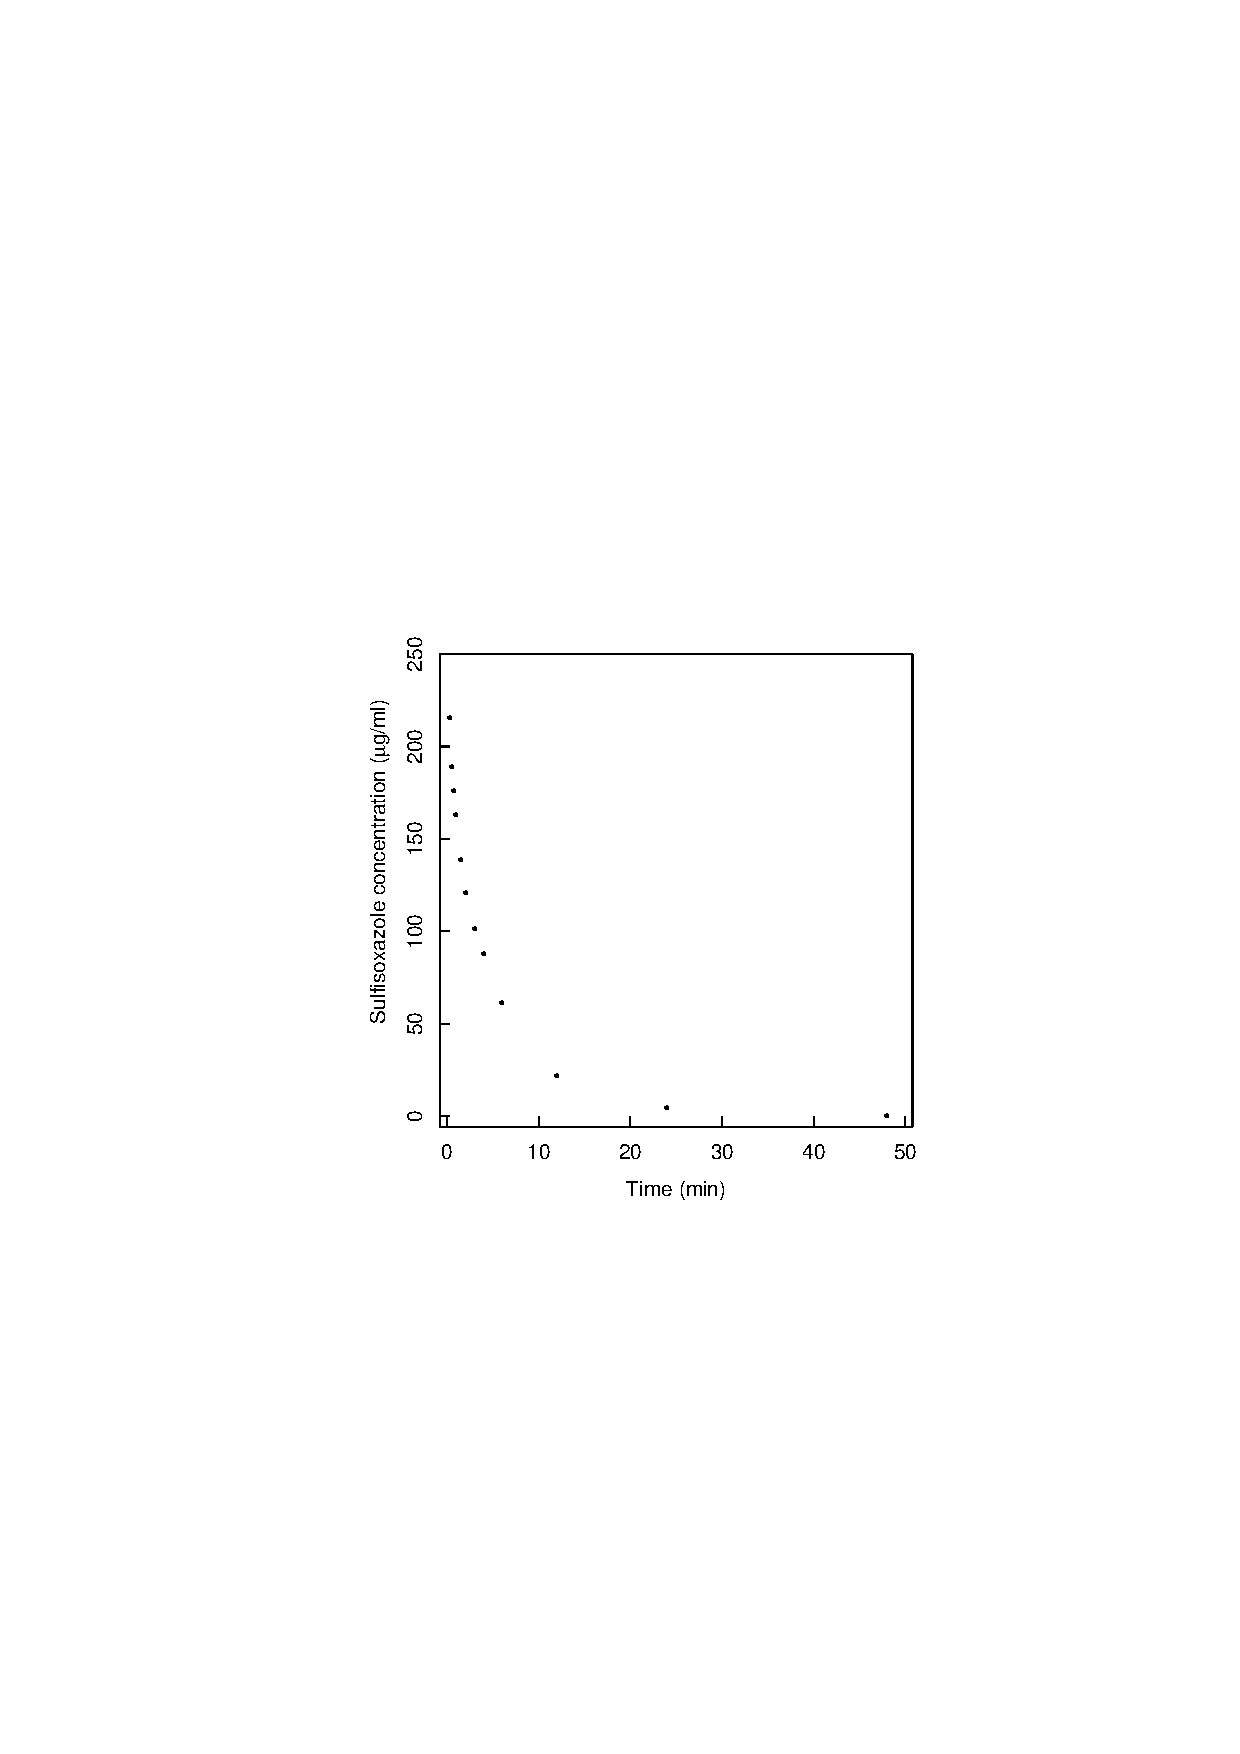
\includegraphics{3SULFdata}}
  \caption{\label{fig:SULFdata}
    Plot of sulfisoxazole concentration in plasma versus time.}
\end{figure}

Plotting the sulfisoxazole concentration on a log scale versus $x$ as
\begin{figure}
  \centerline{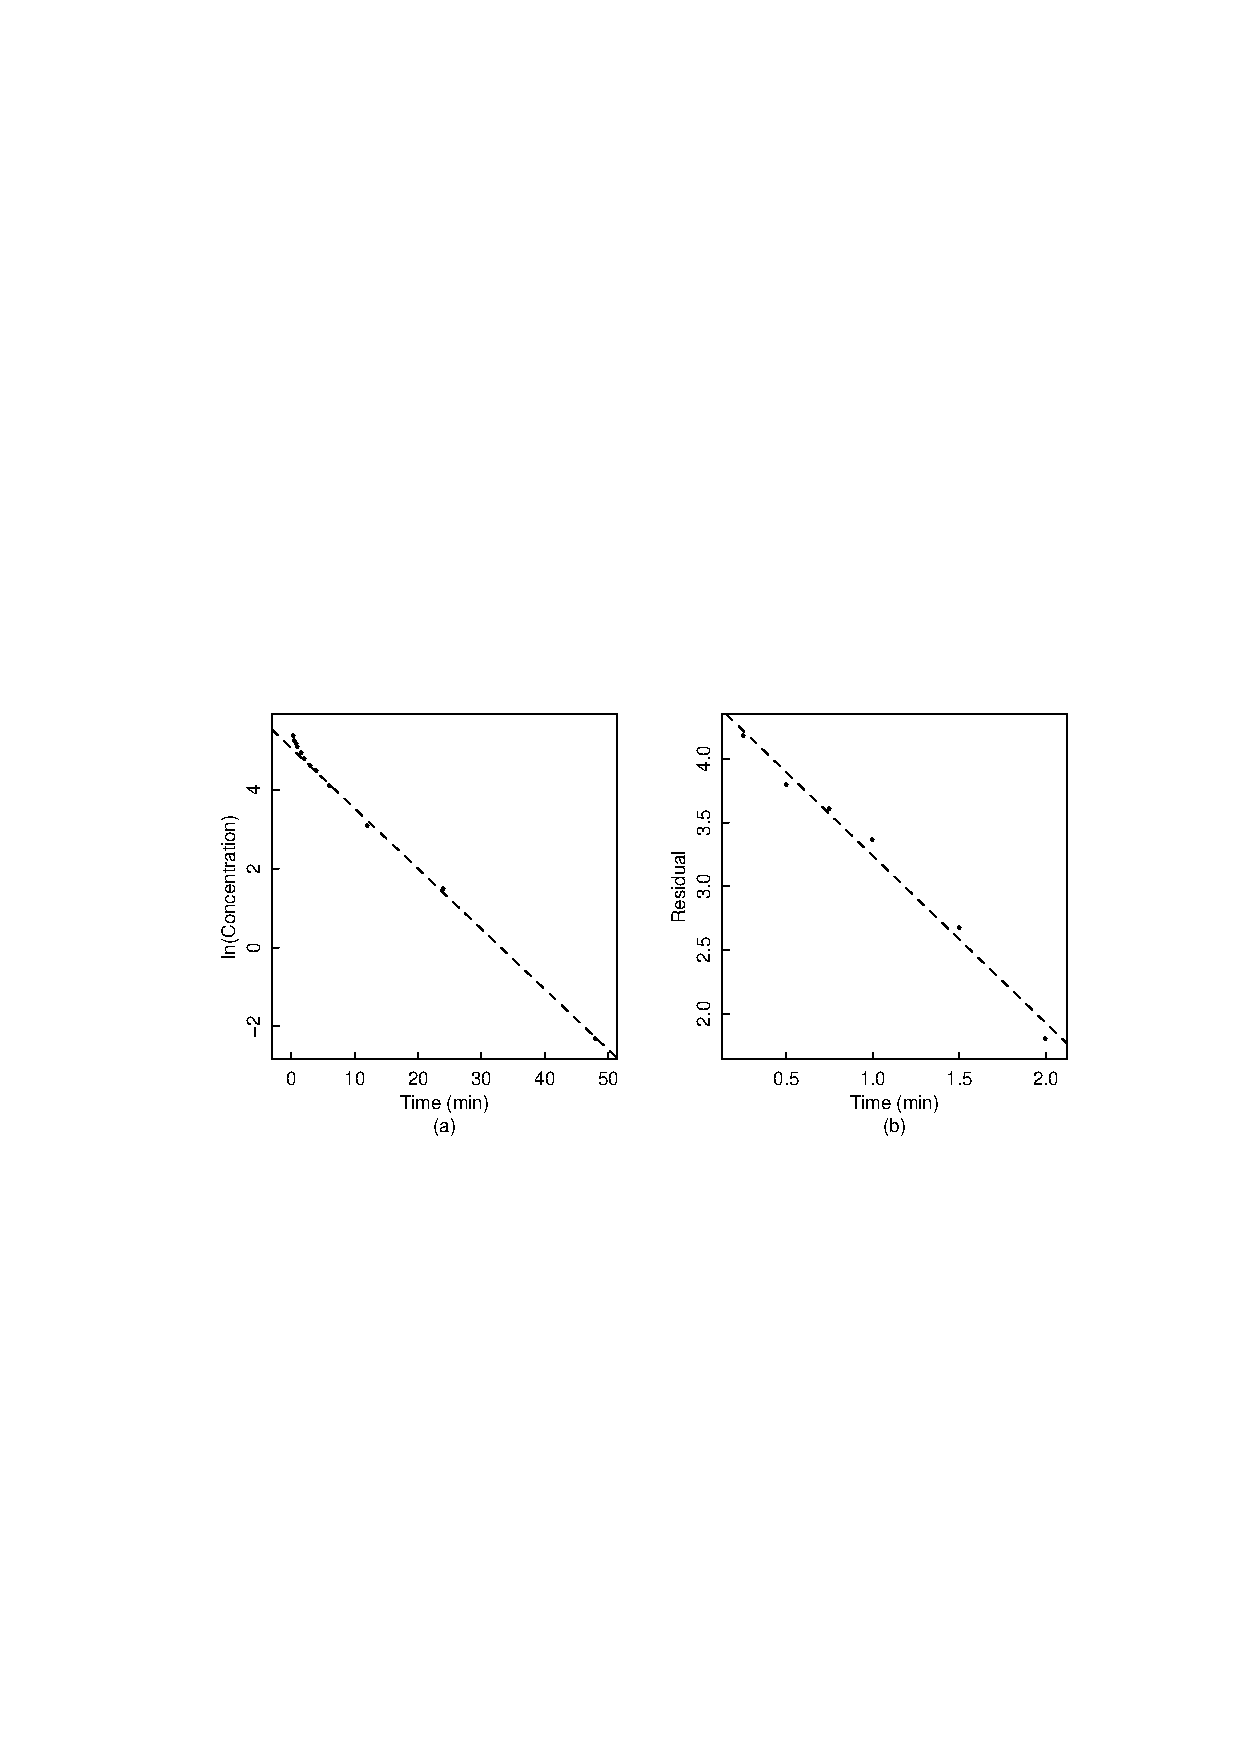
\includegraphics{3SULFstart}}%,width=\textwidth}}
  \caption[Sulfisoxazole curve peeling]{\label{fig:SULFstart}
    Curve peeling using the Sulfisoxazole data.
    In part $a$ we show the data, plotted on a log scale, together with a
    straight line fit (dashed line) to the last six points.
    In part $b$ we show, on a log scale, the residuals for the first six
    data points from the straight line fit in part $a$.
    The dashed line is the fitted line through these (log) residuals.}
\end{figure}
in Figure~\ref{fig:SULFstart}$a$ reveals monotonic decay with straight
line behavior for large $x$, which suggests a model of the form
\begin{displaymath}
  f(x,\btheta)=\theta_1 e^{-\theta_2 x}+\theta_3e^{-\theta_4 x}
\end{displaymath}
with all positive parameters.
Fitting a straight line to the last six (log) data values gives an
intercept of 5.05 and a slope of $-0.153$, so that the
starting values are $\theta_3^{0}= e^{{5.05}}=156$ and
$\theta_4^0 = 0.153$.
Calculating the residuals
\begin{displaymath}
  \tilde y_n = y_n - 156  e^{ - 0.153  x_n }
\end{displaymath}
and plotting $\ln  \tilde y $ versus $x$
for the first six data values, as in Figure~\ref{fig:SULFstart}$b$,
again reveals straight line behavior.
Fitting a straight line to these (log) residuals gives an
intercept of 4.55 and a slope of $-1.31$, so that the
starting values are $\theta_1^0=e^{4.55}=95$ and
$\theta_2 = 1.31$.
\end{example}

\subsection{Reducing Dimensions}
\index{starting values!reducing dimensions}

Peeling is an example of the general technique of reducing dimensions
in order to obtain starting values.  In this technique one estimates
parameters successively, each estimated parameter making it easier to
estimate the remaining ones.  As another example of reducing parameter
dimensions, consider the model
$f = \theta_1 + \theta_2 e^{ - \theta_3 x }$,
where $\theta_{3}$ is positive.  Then the
limiting value of the response when $x\to\infty$ is $\theta_{1}$ and
the value at $x=0$ is $\theta_1+\theta_{2}$.  Depending on
whether the data is increasing or decreasing, we can use
$y_{\mbox{\rm max}}$ or $y_{\mbox{\rm min}}$ to get the starting value
$\theta_1^0$, and then use the difference
$ y ( 0 ) - \theta_1^0 $ to get
$\theta_2^0$.
We perform a linear regression (without a constant term) of
$\ln [ ( y - \theta_1^0 ) / \theta_2^0 ]$ on $x$
to obtain $\theta_3^0$.  Alternatively, once
$\theta_1^{0}$ and $\theta_2^{0}$ are determined, we could
substitute these values into the function and evaluate
$(1/x) \ln [ ( y - \theta_1^0 )/ \theta_2^0 ]$
at selected values of $x$ to obtain $\theta_3^0$.

Sometimes we can reduce the dimensionality of the model and
indirectly reduce the number of parameters.
For example, with the model
$f ( \bx , \btheta )=
\exp [ - \theta_1 x_1 \exp ( - \theta_2 / x_2 )]$,
if there are some very large values of $x_{2}$, then the model
is approximately
$f ( x_1 , \btheta ) = e^{ - \theta_1 x_1 }$, so it is
easy to obtain a starting estimate for $\theta_{1}$ by taking
logarithms of the responses at large $x_{2}$.
Similarly the model
$f ( \bx , \btheta ) = \theta_1 \theta_2 x_1 /
( 1 + \theta_2 x_1 + \theta_3 x_2 )$ reduces
to a Michaelis--Menten type when $x_{2}$ is small, so it is easy
to obtain starting values.
\subsection{Conditional Linearity}
\index{starting values!conditionally linear model}

In many model functions, several of the parameters are conditionally linear
(see Section 2.1) and linear regression can be used to get
starting values for these parameters conditional on the nonlinear
parameters.
Alternatively, special algorithms
which exploit the conditional linearity, described in Section 3.5.5,
can be used.
These algorithms only require starting estimates for the
nonlinear parameters.
As an example of conditional linearity, in
      \begin{displaymath}
        f ( x ,  \btheta ) = \theta_1 + \theta_2 e^{ - \theta_3 x }
      \end{displaymath}
both $\theta_{1}$ and $\theta_{2}$ are conditionally linear,
so it is possible to use linear least squares to estimate
$\theta_1^{0}$ and $\theta_2^{0}$ once an estimate for
$\theta_3^{0}$ has been obtained.
A detailed example involving conditionally linear parameters
\index{parameter!conditionally linear}
is given in Section 3.6.

\section{Parameter Transformations}

As will be shown in Chapters 6 and 7, transforming the parameters in a
nonlinear regression model can produce a much better linear
approximation.  This has the beneficial effects of making approximate
inference regions better and speeding convergence to the least squares
value.  Parameter transformations can also be used to enforce
constraints on the values of the parameters.

Note that transformations of parameters are very different from
transformations of the responses.  Transformations of the response
distort the response space and create a new expectation surface,
thereby affecting the disturbances and the validity of the assumptions
on the disturbances.  In contrast, transformations of the parameters
merely relabel points in the parameter space and on the existing
expectation surface.  Consequently they do not affect the assumptions
about the deterministic or the stochastic parts of the model, although
they do affect the validity of the linear approximation and inferences
based on it.

The use of parameter transformations to improve validity of the linear
approximation is discussed in Chapter 7; here we focus on
transformations to impose constraints on parameters and to improve
convergence.

\subsection{Constrained Parameters}
\index{practical considerations!constraint on parameter}
\index{parameter!constraint}
\index{constraint!on parameter}

The parameters in
most nonlinear models are restricted to regions which make sense
scientifically.
For example, in the Michaelis--Menten model
and in the isomerization model, all the parameters must be
positive, and
in exponential models, the parameters in the exponent
usually must be positive.

It is often possible to ignore the restrictions when fitting
the model and simply examine the converged parameter
estimates to see if they satisfy the constraints.
If the model fits the data well, the parameter estimates should
be in a meaningful range.
Sometimes, though, it may be dangerous to allow the
parameter estimates to go into proscribed regions
during the iterations because the parameter values
may begin to oscillate wildly or
cause numerical overflows.
In these situations, one should impose the constraints throughout the
estimation process.

General techniques for optimizing functions whose parameters are
constrained, called \emph{nonlinear programming}, are beyond the
scope of this book.
See, for example, \citeasnoun{gill:murr:wrig:1981} or
\citeasnoun{bard:1974} for details.
%\glossary{ Gill, P.E.}
%\glossary{ Murray, W.}
%\glossary{ Wright, M.H.}
%\glossary{ Bard, Y.}
Fortunately, the types of constraints that are applied to the parameters of a
nonlinear regression model are usually simple enough to be
handled by parameter transformations.
For example, if $\theta_p $ must be positive, we
reparametrize to $ \phi_p = \ln\theta_p $,
so throughout the iterations
the value of $\theta_p = e^{ \phi_p }$ remains positive.

An \emph{interval} constraint on a parameter, say
\index{constraint!interval}
  \begin{displaymath}
    a  \le  \theta  \le  b
  \end{displaymath}
can be enforced by
a logistic transformation of the form
  \begin{displaymath}
    \theta = a + \frac{b-a}{1 + e^{ - \phi }}
  \end{displaymath}
while an \emph{order} constraint
\index{constraint!order}
on parameters $\theta_j ,\ldots, \theta_{k}$, say
  \begin{displaymath}
    a  \le  \theta_j  \le  \theta_{j+1}  \le  \cdots  \le  \theta_k  \le  b
  \end{displaymath}
can be enforced by a transformation given in \citeasnoun{jupp:1978}.
%\glossary{ Jupp, D.L.B.}

The order constraint can be used to ensure a unique optimum in a model with
exchangeable parameters.
\index{parameter!exchangeable}
As an example of such a model, consider the double exponential model
  \begin{displaymath}
    f ( x , \btheta ) = \theta_1 e^{ - \theta_2  x} +
\theta_3 e^{ - \theta_4  x } 
0 \le \theta_2 ,  \theta_4
  \end{displaymath}
where the pairs of parameters $ ( \theta_1 , \theta_2 )$
and $( \theta_3 , \theta_4 )$ are
\emph{exchangeable}---that is, exchanging the parameter pair
$(\theta_1,\theta_2)$ with the pair $(\theta_3,\theta_4)$ will not 
alter the values of the expected responses.
Exchangeable parameters can create nasty optimization
problems because the linear approximation cannot account for that
kind of symmetry.

In this example, we remove the exchangeability by requiring
  \begin{displaymath}
    0  \le  \theta_2  \le  \theta_4
  \end{displaymath}
and enforce this with the transformation
  \begin{displaymath}
    \theta_2 =e^{ \phi_2 }
  \end{displaymath}
  \begin{displaymath}
    \theta_4 =e^{ \phi_2 }( 1 + e^{ \phi_4 } )
  \end{displaymath}
Since $\theta_{1}$ and $\theta_{3}$ are
conditionally linear parameters, their optimal values are
uniquely determined when $\theta_{2}$ and $\theta_{4}$ are
distinct.
Thus we only need to keep $\theta_{2}$ and $\theta_{4}$ ordered
to eliminate the exchangeability.
\subsection{Facilitating Convergence}
\index{practical considerations!improving convergence}
\index{parameter transformation!to improve convergence}

Parameter transformations can facilitate convergence because they
prevent the parameters from venturing into proscribed regions.
Transformations can also improve convergence by making the
parameter lines behave more uniformly on the expectation surface
so that the Gauss increment is more accurate.
Joint variable--parameter
transformations can also be used to
improve the estimation situation by improving conditioning of
the derivative matrix $\bV$.
\index{derivative matrix!conditioning}
Frequently this is done
by \emph{centering} or \emph{scaling} the data.
\index{parameter transformation!centering and scaling}
\index{improving convergence!centering and scaling}
For example, the simple model
$f ( x , \btheta ) = \theta_1 e^{ - \theta_2  x }$ has derivatives
\begin{displaymath}
  \frac{\partial f}{\partial \theta_1}=e^{-\theta_2 x}
\end{displaymath}
\begin{displaymath}
  \frac{\partial f}{\partial\theta_2}=-x\theta_1e^{-\theta_2 x}
\end{displaymath}
and the derivative vectors tend to be collinear when the values
\index{practical considerations!collinearity}
\index{collinearity}
of $x$ are all positive.
Rewriting the model as
\begin{displaymath}
  f(x,\btheta)=\theta_1 e^{-\theta_2(x-x_0+x_0)}
\end{displaymath}
and reparametrizing with
\begin{displaymath}
  \phi_1=\theta_1e^{-\theta_2 x_0}
\end{displaymath}
\begin{displaymath}
  \phi_2=\theta_2
\end{displaymath}
gives $f(x,\bphi)=\phi_1e^{-\phi_2(x-x_0)}$,
and now the derivatives with respect to $\bphi$ will be more
nearly orthogonal.
A useful choice is $x_0=\bar{x}$.

\emph{Scaling} the variables and the parameters can
also improve conditioning by making the derivative matrix have
column vectors which are more nearly equal in length.

Other transformations can be useful, depending on the context of
the problem.
For example, in chemical kinetics it is often useful to revise
the model so that reciprocal absolute temperature is used rather
than temperature $T$.
Combining this with centering would then modify a term involving
temperature to the form
$1/T-1/T_{0}$.

The effect of parameter transformations on parameter effects
nonlinearities and the adequacy of linear approximation inference
regions is discussed in Chapter 7.

\section{Other Iterative Techniques}

The Gauss--Newton iterative algorithm for nonlinear least squares,
described in Section 2.2.1, is a simple, useful method for
finding $\hat{\btheta}$.
Some modifications to this method, as well as alternative methods,
have been suggested---primarily to deal with ill-conditioning of
the derivative matrix $\bV$ and to avoid having to
code and specify the derivatives.
\subsection{A Newton--Raphson Method}

The Gauss--Newton method for estimating nonlinear parameters can be
\index{Gauss-Newton!iteration method}
considered as a special case of the more general Newton--Raphson method
\index{Newton-Raphson!iteration method}
\cite{bard:1974} which uses a local quadratic approximation to the
%\glossary{ Bard, Y.}
objective function.
Near $\btheta^{0}$, we approximate
\begin{displaymath}
  S ( \btheta ) \approx S ( \btheta^0 )
  + {\bomega} \trans ( \btheta - \btheta^0 )
  + ( \btheta - \btheta^0 )\trans\frac{\bOMEGA}{2}(\btheta-\btheta^0)
\end{displaymath}
where
\begin{displaymath}
  \bomega  = \frac{\partial S}{\partial \btheta}
\end{displaymath}
is the \emph{gradient}
\index{gradient!of sum of squares function}
of $S ( \btheta )$ evaluated at $\btheta^{0}$
and
\begin{displaymath}
  \bOMEGA=\frac{\partial^2 S}{\partial\btheta\partial\btheta\trans}
\end{displaymath}
is the \emph{Hessian}
\index{Hessian!of sum of squares function}
of $S(\btheta)$ evaluated at $\btheta^{0}$.
The approximating sum of squares function will have
a stationary point when its gradient is zero---that is, when
\begin{displaymath}
  \bomega+\bOMEGA(\btheta-\btheta^0)=\bm0 
\end{displaymath}
and this stationary point will be a minimum if $\bOMEGA$ is positive
definite (all its eigenvalues positive).
If $\bOMEGA$ is positive definite, the Newton--Raphson step is
\begin{displaymath}
  \bdelta^0=-\bOMEGA^{-1}\bomega .
\end{displaymath}

For the function
\begin{displaymath}
  S(\btheta)=(\by-\boeta)\trans(\by-\boeta)
\end{displaymath}
the gradient is
\begin{displaymath}
  \bomega=-2\bV\trans(\by-\boeta)
\end{displaymath}
and the Hessian is
\begin{displaymath}
  \bOMEGA=2\bV\trans\bV-2\frac{\partial\bV\trans}{\partial\btheta\trans}(\by-\boeta)
\end{displaymath}
where $\bV$ is the derivative matrix.
The Gauss--Newton increment is therefore equivalent to the
Newton--Raphson increment with the second derivative term
${\partial\bV\trans}/{\partial\btheta\trans}$ set to zero.

\citeasnoun{denn:gay:wels:1981} describe a nonlinear least squares
%\glossary{ Dennis, J.E.Jr.}
%\glossary{ Gay, D.M.}
%\glossary{ Welsch, R.E.}
routine which develops a quasi-Newton approximation \cite{denn:schn:1983}
to the second term in the Hessian.
%\glossary{ Dennis, J.E.Jr.}
%\glossary{ Schnabel, R.B.}
This extends the Gauss--Newton algorithm and makes it closer to the
Newton--Raphson algorithm,
which has the advantage that the approximating Hessian should be closer
to the actual Hessian than the single term $\bV \trans \bV$ used in
the Gauss--Newton algorithm.
However, the term $\bV \trans \bV$ is necessarily positive definite
(or at least positive semidefinite),
since the eigenvalues of $\bV \trans \bV$ are the squares of the singular
values of $\bV$.
Adding another term on to this to form an approximating
Hessian can destroy the positive definiteness, in which case the
Newton--Raphson algorithm must be modified to restore
positive definiteness in the Hessian.
\subsection{The Levenberg--Marquardt Compromise}
\index{practical considerations!Levenberg--Marquardt compromise}
\index{Levenberg--Marquardt compromise}

A condition that can cause erratic behavior of Gauss--Newton
iterations is singularity of the derivative
matrix $\bV$ caused by collinearity of the columns.
\index{practical considerations!collinearity}
\index{collinearity}
When $\bV$ is nearly singular,
$\bdelta$ can be very large, causing the parameters to go into
undesirable regions of the parameter space.

One solution to the problem of near-singularity is to perform the
calculations for the increment in a numerically stable way, which is why
we recommend using the $QR$ decomposition rather than
\index{practical considerations!QR decomposition}
the normal equations.
We also recommend using double precision or extended
precision arithmetic for the calculations, where feasible, and
using joint variable--parameter transformations as discussed in
Section 3.4.

Another general method for dealing with near-singularity is
to modify the Gauss--Newton increment to
  \begin{displaymath}\label{eqn:levenberg}
    \bdelta (k)=( \bV \trans \bV+k \bI )^{-1}
    \bV \trans ( \by - \boeta )
  \end{displaymath}
as suggested in \citeasnoun{leve:1944}, or to
%\glossary{ Levenberg, K.}
  \begin{displaymath}\label{eqn:marquardt}
    \bdelta (k) = ( \bV \trans \bV + k \bD )^{-1}
    \bV \trans ( \by - \boeta )
  \end{displaymath}
as suggested in \citeasnoun{marq:1963}, where $k$ is a conditioning factor
%\glossary{ Marquardt, D.W.}
and $\bD$ is a diagonal matrix with entries equal to the
diagonal elements of $\bV \trans \bV$.
This is called the \emph{Levenberg--Marquardt compromise}
because
\index{practical considerations!Levenberg--Marquardt compromise}
\index{Levenberg--Marquardt compromise}
the direction of $\bdelta (k)$ is intermediate between the direction
of the Gauss--Newton increment ($k\to 0$)
\index{Gauss-Newton increment}
and the direction of \emph{steepest descent}
\index{steepest descent}
$\bV\trans(\by-\boeta)/\norm\bV\trans(\by-\boeta)\norm$ ($k\to\infty$).

Note that Levenberg recommends inflating the diagonal of
$\bV \trans \bV$ by an additive factor, while Marquardt recommends
inflating the diagonal by a multiplicative factor $1 + k$.
Marquardt's method produces an increment which is invariant under
scaling transformations of the parameters, so that
if the scale for one component of the parameter
vector is doubled, the increment calculated, and the
corresponding component of the increment halved, the result
will be the same as calculating the increment in the original
scale.
In Levenberg's method, this is not true.
\citeasnoun{box:kane:1984} showed, however, that if one
%\glossary{ Box, G.E.P.}
%\glossary{ Kanemasu, H.}
requires invariance of the increment under linear
transformations of the parameter space, the resulting increment is the
Gauss--Newton increment with a step factor.

The Levenberg--Marquardt compromise is more difficult to implement
than the Gauss--Newton algorithm, since one must decide
how to manipulate both the conditioning factor $k$ and the step
factor $\lambda$; nevertheless
it is implemented in many nonlinear least squares programs.
Although we presented the increment in terms of the inverse of an
augmented $\bV \trans \bV$ matrix, the actual calculations for the
increment should be done using a $QR$ decomposition of $\bV$ and
applying updates from a diagonal matrix using the Givens
rotations \cite{golu:pere:1973,dong:bunc:mole:stew:1979}, (Chapter 10),
%\glossary{ Golub, G.H.}
%\glossary{ Pereyra, V.}
%\glossary{ Dongarra, J.J.}
%\glossary{ Bunch, J.R.}
%\glossary{ Moler, C.B.}
%\glossary{Stewart, G.W.}
since the Levenberg increment (\ref{eqn:levenberg}) is the least squares
solution to the system with derivative matrix
\begin{displaymath}
  \begin{bmatrix}\bV\\\sqrt k\bI \end{bmatrix}
\end{displaymath}
and response vector
\begin{displaymath}
  \begin{bmatrix}\by-\boeta\\\bm0\end{bmatrix}
\end{displaymath}
For the Marquardt increment (\ref{eqn:marquardt}), the derivative matrix
is changed to
\begin{displaymath}
  \begin{bmatrix}\bV\\\sqrt k\bD^{1/2}\end{bmatrix}
\end{displaymath}
\subsection{Numerical Derivatives}
\index{practical considerations!numerical derivatives}

We have assumed that implementations of the algorithms we have
described use analytic derivatives with respect to the parameters.
Obtaining these derivatives and coding them
is usually the most tedious and error-prone stage in a
nonlinear analysis.

As a general rule we recommend using analytic derivatives for
accuracy, although it is convenient to use programs which use
numerical derivatives from finite differences.
Such convenience is not obtained without cost, however, because
numerical derivatives can be inaccurate and they usually increase the
computing time necessary to obtain convergence.
Furthermore, if second derivatives are required to investigate the
effect of nonlinearity on inferences, the numerical second derivatives
evaluated from numerical first derivatives can be very
inaccurate.
Other problems with numerical derivatives involve the choice of
step size to determine the finite differences, and whether to use
central or forward differences.

With forward differences, for the $p$th
parameter we evaluate the model function
using the current values of all the
parameters except for the $p$th, which is incremented
to $\theta_p ( 1 + \epsilon )$.
Dividing the differences between the function values
by the fractional amount $\epsilon \theta_{p}$
gives an approximate derivative.
This requires $1 + P$ evaluations of the expected response
vector at each iteration.
Using central differences would require evaluation of the model
function at
$\theta_p ( 1 \pm \epsilon )$ in addition to the central
value, so the total number of evaluations would be
$1 + 2 P$.
%{.dennis schnabel 1983.}
Dennis and Schnabel (1983) recommend setting $\epsilon$ equal to the
%\glossary{ Dennis, J.E.Jr.}
%\glossary{ Schnabel, R.B.}
square root of the relative machine precision (that is, the square
root of the smallest number which, when added to 1.0 in
the floating point arithmetic of the computer, produces a number
greater than 1.0).
\subsection{Derivative-Free Methods}
\index{practical considerations!derivative-free methods}

There are derivative-free methods which do not simply use
numerical approximations to derivatives.
\citeasnoun{rals:jenn:1978} introduced one such routine, DUD
%\glossary{ Ralston, M.L.}
%\glossary{ Jennrich, R.I.}
\index{DUD}
(Doesn't Use Derivatives), which is
based on using a secant plane approximation to the
expectation surface rather than a tangent plane approximation.

To use DUD, one must provide starting values $\btheta^{0}$.
The program then automatically produces a further set of $P$ parameter
vectors by displacing each parameter in turn by 10\%.
These parameter vectors are then used to calculate expectation
vectors $\boeta_{1}$, $\boeta_2 ,\ldots,$ giving a
secant plane which matches the expectation surface at
$P + 1$ points.
A set of linear coordinates is generated on the secant plane, and
the projection of $\by$ onto the secant plane is made and
mapped into the parameter plane.
This information is used to calculate a new $\btheta$ vector,
say $\btheta '$, for which $\boeta ( \btheta ' )$ is
closer to $\by$ than any of the other parameter vectors.
The parameter vector $\btheta$ corresponding to the
$\boeta$ which is farthest from $\by$ is then replaced by
$\btheta '$, and the process continued until convergence is
achieved.
\label{rum:dud}
\begin{example}

DUD can be illustrated very effectively using
a two-observation example such as in Example Rumford 2.
To simplify arithmetic and to provide a better scale for the
figure, we provide the necessary two $( = P + 1 )$ starting
values rather than using the automatic 10\% displacement.
The two starting values are chosen to be $\theta^1=0.02$
and $\theta^2=0.10$.
Figure~\ref{fig:RUM2dud} shows the expectation surface
  \begin{figure}
    \vspace{3in}
    \centerline{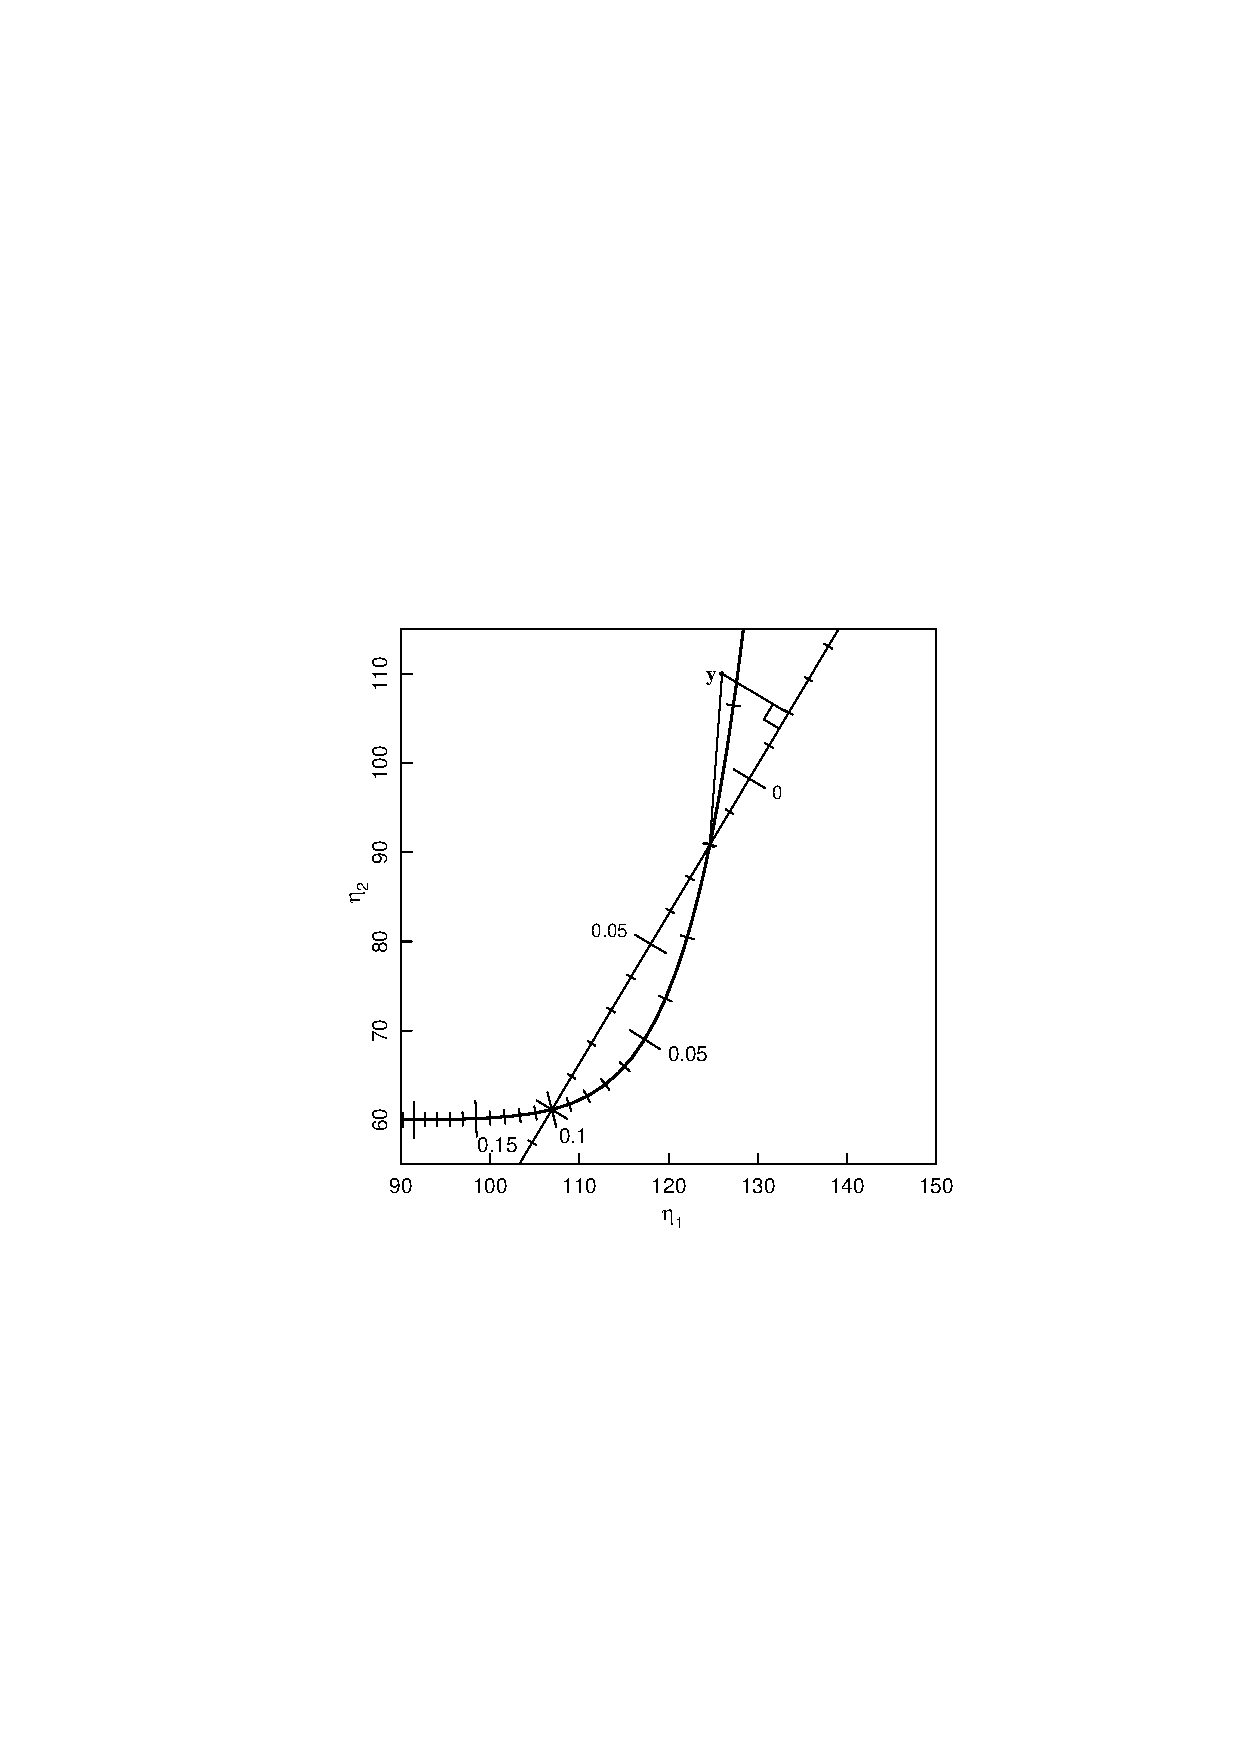
\includegraphics{3RUM2dud}}%,height=3in}}
    \caption[Geometric representation of DUD]{
    A geometric interpretation of the calculation of the DUD
    increment using the 2-case Rumford data.
    A portion of the expectation surface (heavy solid line) is shown in
    the response space together with the observed response $\by$.
    Also shown is the projection of $\by-\boeta ( 0.02 )$ onto the
    secant plane joining $\boeta ( 0.02 )$ and $\boeta ( 0.10 )$
    (solid line).
    The tick marks indicate true positions on the expectation surface and
    linear approximation positions on the secant plane.
    }
    \label{fig:RUM2dud}
  \end{figure}
$\boeta ( \theta )$ together with the secant line
$\bl$ through the points
$\boeta ( \theta^1 )$ and $\boeta ( \theta^2 )$.
We now introduce a linear scale parameter $\alpha$ on $\theta$ such
that $\theta =\theta^1+T\alpha$, where
$T = (\theta^2-\theta^1)$ and so $\alpha=0$ at
$\theta^{1}$ and $\alpha = 1$ at $\theta^{2}$.
We also impose a linear scale on $\bl$ such that
$\bl ( \alpha )=\boeta ( \theta^1 )+\bH \alpha$,
where $\bH=\boeta ( \theta^2 )-\boeta ( \theta^1 )$.
The linear coordinate system is also shown in Figure~\ref{fig:RUM2dud}.

For this example, $T=\theta^2-\theta^1=0.08$,
$\theta=\theta^1+T\alpha$, so 
\begin{displaymath}
  \alpha =\frac{\theta-\theta^1}{T}
\end{displaymath}
\begin{eqnarray*}
  \bH&=&
  \begin{bmatrix}
    60+70e^{{-4(0.1)}}\\
    60+70e^{ -41(0.1)}
  \end{bmatrix} -
  \begin{bmatrix}
    60+70e^{-4(0.02)}\\
    60+70e^{-41(0.02)}
  \end{bmatrix}\\
  &=&\begin{bmatrix}106.92 \\ 61.16\end{bmatrix} -
  \begin{bmatrix}124.62 \\ 90.83\end{bmatrix}\\
  &=&\begin{bmatrix}-17.70 \\ -29.67\end{bmatrix}
\end{eqnarray*}
and
\begin{eqnarray*}
  \bl&=&\boeta ( \theta^1 )+\bH \alpha\\
  &=&\begin{bmatrix}124.62 \\ 90.83\end{bmatrix} +
  \begin{bmatrix}-17.70 \\ -29.67\end{bmatrix}
  \alpha
\end{eqnarray*}
We now use linear least squares to project the residual vector
\begin{eqnarray*}
  \by-\bl (0)&=&\begin{bmatrix}126 \\ 110\end{bmatrix} -
  \begin{bmatrix}124.62 \\ 90.83\end{bmatrix}\\
  &=&\begin{bmatrix}1.38 \\ 19.17\end{bmatrix}
\end{eqnarray*}
onto $\bl$ to obtain
\begin{displaymath}
  \hat{\alpha}=( \bH \trans \bH )^{-1}
  \bH \trans ( \by - \bl ( 0 ) )
\end{displaymath}
For this example
\begin{displaymath}
  \hat{\alpha}=-0.49
\end{displaymath}
so new value of $\theta$ is
\begin{eqnarray*}
  \theta_{\mbox{\rm new}}&=&0.02+T ( - 0.49 )\\
  &=&0.02 + 0.08 ( -0.49 )\\
  &=&-0.019
\end{eqnarray*}
Evaluating the sum of squares at this point reveals that this new
point is farther from $\by$ than either of the two starting
points, and so a step factor $\lambda$ is introduced to
\index{step factor}
search along the increment vector to determine a better point.
Incorporating $\lambda$ as
  \begin{displaymath}
    \theta_{\mbox{\rm trial}} = \theta_{\mbox{\rm new}} \lambda +
    \theta_{\mbox{\rm old}} ( 1 - \lambda )
  \end{displaymath}
gives, for this example,
  \begin{displaymath}
    \theta_{\mbox{\rm trial}} = (- 0.019) \lambda + 0.02 ( 1 - \lambda )
  \end{displaymath}
and the minimum occurs at $\lambda = 0.5$ with
$\theta_{\mbox{\rm trial}} = 0.0005$.
The point $\theta^2=0.10$ is then replaced by $\theta^3=0.0005$
and the process is repeated using the pair
$( \theta^1 , \theta^3 )$.
\end{example}

In the general case of $P$ parameters, at the $i$th iteration
we use the values of $\boeta ( \btheta )$ at
$\btheta_1^i , \btheta_2^i ,\dots, \btheta_{P+1}^{i}$
to determine the secant plane
as the $P$-dimensional plane which passes through
$\boeta ( \btheta_p^i )$, $p = 1 ,\ldots, P+1$.
For convenience, we assume that $\btheta_{P+1}^{i}$
corresponds to the point closest to $\by$;
we then determine the $P\times P$
matrix $\bT$ by setting its $p$th column
equal to $\btheta_p^i - \btheta_{P+1}^{i}$,
and the $N\times P$
matrix $\bH$ by setting its $p$th column equal to
$\boeta ( \btheta_p^i ) -
\boeta ( \btheta_{P+1}^i )$.
Then, formally,
\begin{eqnarray*}
  \hat{\balpha}&=&( \bH \trans \bH )^{-1} \bH \trans
  [ \by - \boeta ( \btheta_{P+1}^i ) ]\\
  \btheta_{\mbox{\rm new}}&=&\btheta_{P+1}^i + \bT \hat{\balpha}
\end{eqnarray*}
and
\begin{displaymath}
  \btheta_{\mbox{\rm trial}} = \btheta_{\mbox{\rm new}}\lambda+
  \btheta_{P+1}^i (1-\lambda)
\end{displaymath}
Note that
\citeasnoun{rals:jenn:1978} allow the step factor to be negative,
%\glossary{ Ralston, M.L.}
%\glossary{ Jennrich, R.I.}
\index{step factor}
by choosing $\lambda$ from a sequence of values
$1,1/2,-1/4,1/8,-1/16,\cdots$.
At convergence the linear approximation parameter covariance
\index{parameter!approximate covariance matrix}
matrix is given by $s^2 \bT ( \bH \trans \bH )^{-1} \bT \trans$,
where $s^{2}$ is the usual variance estimate.
Note that the matrix $\bT$ may be
ill conditioned by the time convergence is achieved and so the linear
approximation standard errors and correlations may not be reliable.
\subsection{Removing Conditionally Linear Parameters}

One way of simplifying a nonlinear regression problem is to
eliminate conditionally linear parameters.
\index{conditionally linear!parameter}
\index{parameter!conditionally linear}
\index{practical considerations!conditionally linear parameter}
As mentioned in Sections 2.1 and 3.3.5,
the optimal values of the conditionally linear
parameters, for fixed values of the nonlinear parameters, can be
determined by linear least squares.
If we partition the parameter vector $\btheta$ into the conditionally
linear parameters $\bbeta$ of dimension $P_{1}$
and the nonlinear parameters $\bphi$ of dimension $P_{2}$ with
$P = P_1 + P_{2}$,
the expected responses can be written
\begin{displaymath}
  \boeta ( \bbeta , \bphi ) = \bA ( \bphi ) \bbeta
\end{displaymath}
where the $N\times P_{1}$ matrix $\bA$ depends only on the
nonlinear parameters.
For any value of $\bphi$, the conditional estimate of $\bbeta$ is
\begin{displaymath}
  \hat{\bbeta} ( \bphi ) = \bA^+ ( \bphi )  \by
\end{displaymath}
where $\bA^+ = ( \bA \trans \bA )^{-1} \bA \trans$
is the pseudoinverse of $\bA$.
The associated expected responses are
\begin{displaymath}
  \hat{\boeta}( \bphi ) = \bA ( \bphi ) \bA^+ ( \bphi )  \by
\end{displaymath}
\citeasnoun{golu:pere:1973} formulated a Gauss--Newton algorithm to minimize
%\glossary{ Golub, G.H.}
%\glossary{ Pereyra, V.}
the reduced sum of squares function
\begin{displaymath}
  S_2 ( \bphi ) =
\norm \by - \bA ( \bphi ) \hat{\bbeta}( \bphi ) \norm^2
\end{displaymath}
that depends only on the nonlinear parameters.
In particular, they give the derivative
of $\bA^+ ( \bphi )$ with respect to $\bphi$, which is the key
ingredient in the algorithm.
The expression for this derivative is used in Chapter 4,
where we present a Gauss--Newton algorithm for multiresponse
parameter estimation.

One difficulty with using projection over the conditionally
linear parameters is that additional information about the
parameters must be given by the user.
The user must specify which parameters are conditionally linear
as well as specifying the derivatives of the entries of $\bA$ with
respect to $\bphi$.
This often results in more difficulty than
simply ignoring the conditional linearity.
There are some structured problems, however---such as spline
regression with knot positions allowed to vary, as described in
\citeasnoun{jupp:1978}---where the division between conditionally linear and
%\glossary{ Jupp, D.L.B.}
nonlinear parameters is inherent in the specification of the
problem, so the Golub--Pereyra method can be used to advantage.
These methods are discussed further in \citeasnoun{kauf:1975} and
%\glossary{ Kaufman L.}
\citeasnoun{bate:lind:1986}.
%\glossary{ Bates, D.M.}
%\glossary{ Lindstrom, M.J.}

\section{Obtaining Convergence}
\index{practical considerations!obtaining convergence}
\index{convergence!practical considerations}

Obtaining convergence is sometimes difficult.
If you are having trouble, check the following:
  \begin{itemize}
    \item Is the expectation function correctly specified?
    \item Is the expectation function correctly coded?
    \item Are the derivatives correctly specified?
    \item Are the derivatives correctly coded?
    \item Are the data entered correctly?
    \item Are all the observations reasonable?
    \item Is the response variable correctly identified?
    \item Do the starting values have the correct values?
    \item Do the starting values correspond to the correct parameters?
  \end{itemize}

If the answer to all these questions
is yes, look carefully
at the output from the optimization program.
Most good programs can produce detailed output on each
iteration to help find out what is wrong.
Check to see that the initial sum of squares, $S ( \btheta^0 )$, is
smaller than the sum of squares of the responses.
If not, then the fitted function is worse than no function
and, in spite of your checks, you probably have an incorrect
expectation function, or incorrect data, or incorrect starting
values.
You may even be trying to fit an $x$ variable rather
than the response $y$.

Look at the parameter values.
Do the starting values have the correct magnitudes?
Correct signs?
And are they assigned to the correct parameters?

Next, look at the parameter increments.
Are they all of roughly the same magnitude relative to the
parameters?
Does the increment, when added to the parameter vector, place the
parameter vector in a bad region in the parameter space?
For example, are any necessarily positive parameters driven
negative?
Do any of the parameters become unreasonably large or small?
If so, could there be an error in the derivative functions?
Try using numerical derivatives at a few design points to check
the analytic derivatives.
Would different starting values for some of the parameters help?
Is there a transformation of the parameters which could help?

Sometimes convergence is not achieved because the model has too
many parameters.
Look at the parameter values to see whether any of them are being
driven to extreme values corresponding to a simpler model function.
Also look at combinations of the parameter increments to see, for
example, if pairs of them tend to move together, suggesting
collinearity or possibly overparametrization.
\index{overparametrization}
If there is a suspicion of overparametrization, try simplifying
the expectation function, even temporarily---it may be that a
simpler model will produce better parameter estimates, so that
eventually the full model can be fitted.

Check to see that there are enough data in all regions of
the design space so that valid parameter estimates can be obtained.
For example, when fitting a transition type model in which there
is, say, linear behavior to the left of a point and different
linear behavior to the right
\cite{baco:watt:1971,hink:1969,watt:baco:1974},
%\glossary{ Bacon, D.W.}
%\glossary{ Watts, D.G.}
%\glossary{ Hinkley, D.V.}
it is often the case that there are
lots of data values to define the behavior away from the join
point, but not many near the join point.
In this situation, the parameter which describes the sharpness of
transition will be poorly estimated, and so convergence may be
slow.

When dealing with a comprehensive model which involves combining
data from several experiments, it is generally good practice to
fit each data set with a possibly simpler restricted model, and
gradually extend the model by incorporating more data sets and
parameters.
An example of this is given in \citeasnoun{zieg:1985}.
%\glossary{ Ziegel, E.R.}
Conversely, a large data set which has several reasonably
distinct operating regions can be blocked into small subsets on
that basis, so that a reduced model can be fitted to each subset
and the results used to provide starting estimates for a model
for the full data set, as illustrated below.
\label{lub:converge}
\begin{example}

To illustrate the process of getting starting values and obtaining
convergence for a complicated nonlinear model function, we consider
data on the kinematic viscosity of a lubricant as a function of
temperature ($x_{1}$) and pressure ($x_{2}$).  The data, discussed
in \citeasnoun{lins:1975}, are reproduced in
%\glossary{ Linssen, H.N.}
Appendix A, Section~\ref{atbl:lub}, and plotted in Figure \ref{fig:LUBdata}.
\begin{figure}
  \vspace{3in}
  \centerline{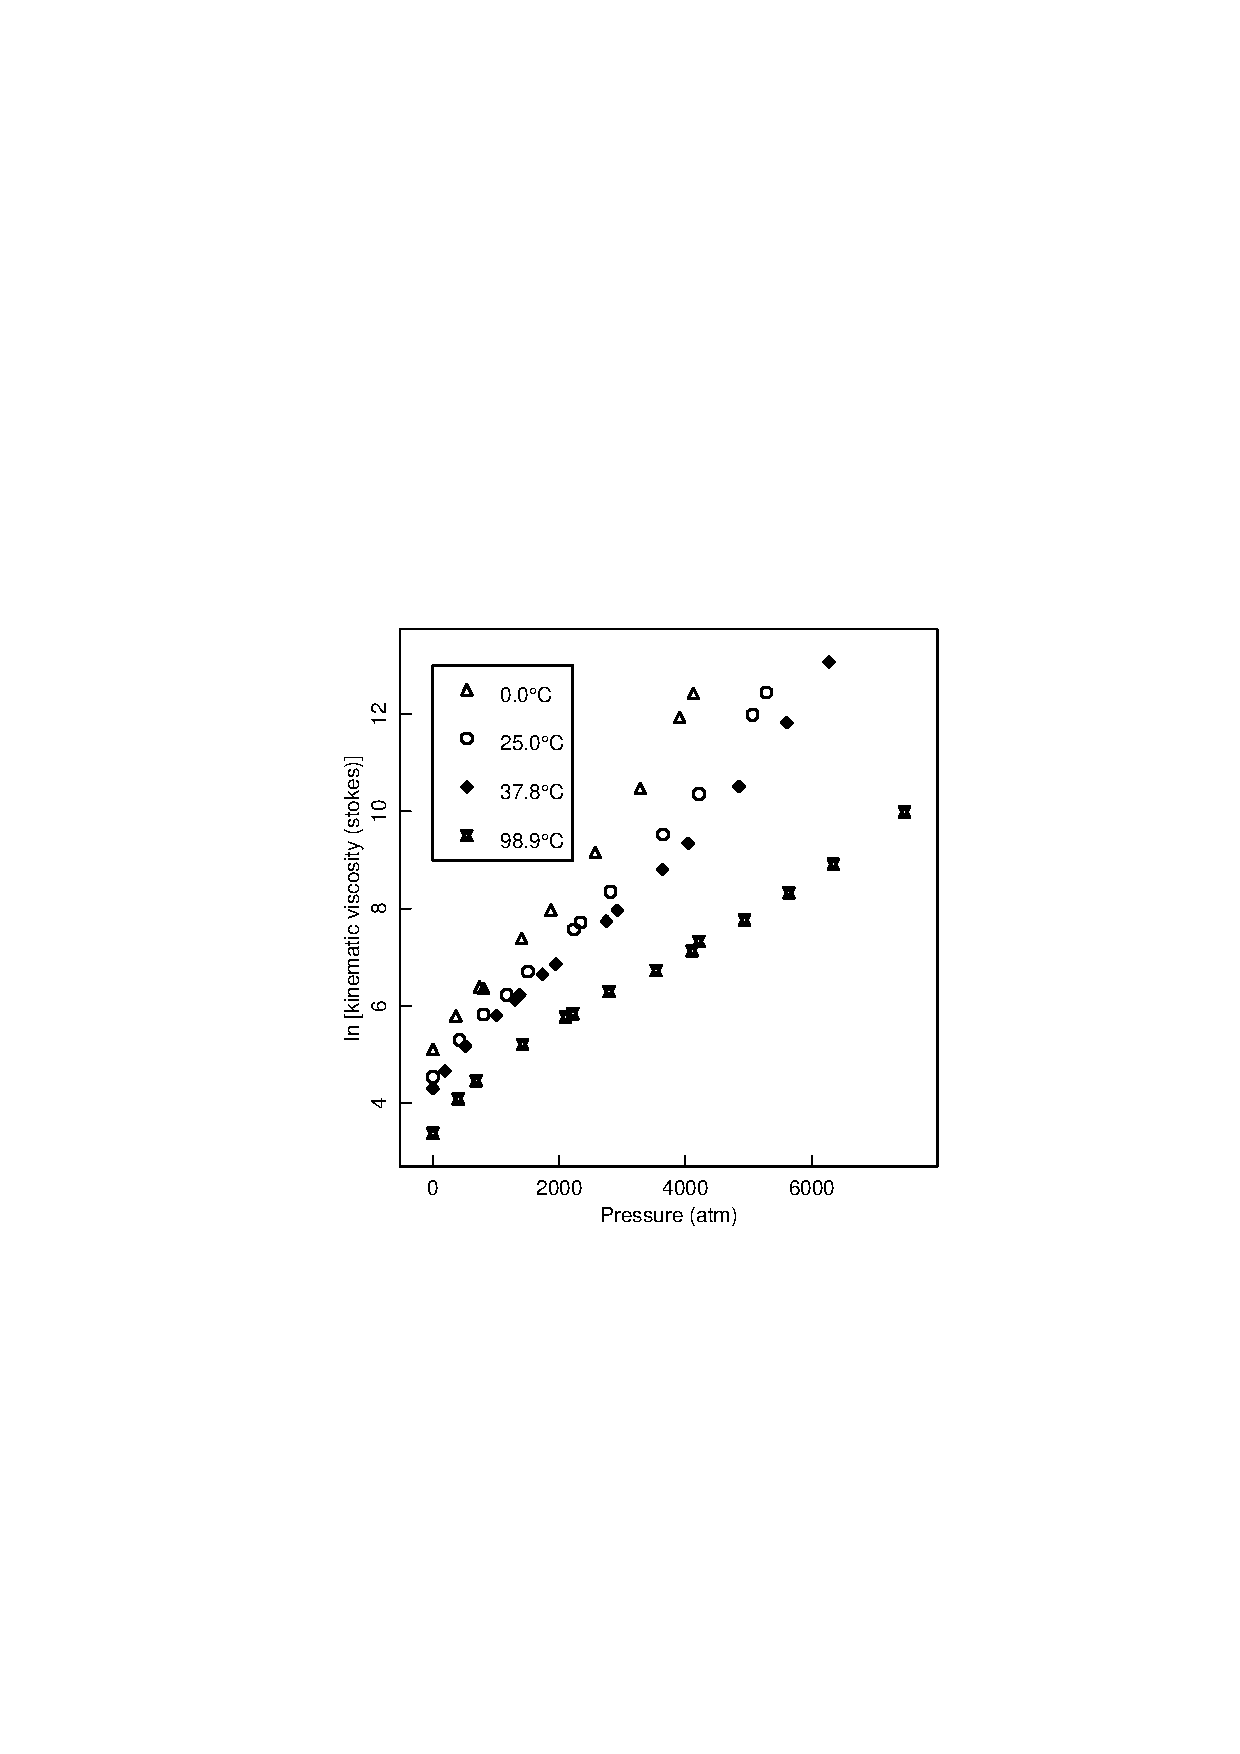
\includegraphics{3LUBdata}}%,height=3in}}
  \caption{
    Plot of the logarithm of the kinematic viscosity of a lubricant versus
    pressure for four different temperatures.
  }\label{fig:LUBdata}
\end{figure}
The model function is
\begin{eqnarray}\label{eqn:lub}
  f (\bx,\btheta)&=&\frac{\theta_1}{\theta_2+x_1}+
  \theta_3 x_2+\theta_4 x_2^2 +
  \theta_5 x_2^3\\
  &&+( \theta_6 + \theta_7 x_2^2 )  x_2 
  \exp \left(\frac{-x_1}{\theta_8+\theta_9 x_2^2}
  \right)\nonumber
\end{eqnarray}

To begin, we note that six of the nine parameters are
conditionally linear, which is most helpful.
Also, to improve conditioning, as discussed in Section 3.4.1, we scale
the pressure data $x_{2}$ by dividing by $1000$ and avoid
confusion by writing $w_2=x_2 / 1000$.

To obtain a starting estimate for $\theta_{2}$, we use the
data for $w_2 = 0.001$ and assume that for this low value of
scaled pressure, the model is a
function of $x_{1}$ only.
Taking reciprocals and using linear least squares as
described in Section 3.3.3 gives $\theta_1^0 = 983$
and $\theta_2^0 = 192$.

Now we exploit the conditional linearity in the model
because we can use linear least squares
to obtain starting estimates for the remaining parameters
once we have reasonable estimates for
$\theta_{8}$ and $\theta_{9}$.
Thus we concentrate on getting estimates for only
these two.
We simplify the situation even more by assuming that
when $w_{2}$ is small,
the model function is essentially linear in $w_{2}$, so that
\begin{displaymath}
  f(\bx,\btheta)\approx\frac{\theta_1}{\theta_2+x_1}+\theta_3w_2+\theta_6w_2e^{-x_1/\theta_8}
\end{displaymath}
That is, we can ignore the terms involving $\theta_{4}$,
$\theta_{5}$, $\theta_{7}$, and $\theta_{9}$.
By examining the plot, we see that the data for each temperature
follow quite straight lines for $w_22$, so we choose
this for the range.
Also, for fixed values of $x_{1}$, the leading term and the
exponential term are constant and we may rearrange the model as
  \begin{eqnarray*}
    y'&=&\theta_3 w_2 + \theta_6 w_2  g\\
    &=&w_2  \beta
  \end{eqnarray*}
where
\begin{displaymath}
  y'=\frac{y-983}{192+x_1}
\end{displaymath}
\begin{displaymath}
g = e^{ - x_1 / \theta_8 }
\end{displaymath}
and
\begin{displaymath}
\beta = \theta_3 + \theta_6 g
\end{displaymath}

Regressing $y'$ on $w_{2}$ for each of the four temperatures
0, 25, 37.8, 98.9 gives $\beta$ values of 1.57, 1.49, 1.39, 1.37.
We now use the $\beta$ values and the relation
$g = e^{ - x_1 / \theta_8 }$
to obtain estimates for $\theta_{3}$ and $\theta_{6}$ by
noting that when $x_1=0$ we have $g=1$,
so $\beta=\theta_3+\theta_{6}$,
and when $x_1\to\infty$ $\beta=\theta_{3}$.
We therefore estimate the sum of the two parameters as 1.57
(the value of $\beta$ at $x_1 = 0$), and
assuming that the lower asymptote has almost been reached at the
highest temperature,
we choose $\theta_{3}$ to be 1.35, which is a bit smaller than 1.37
(the value of $\beta$ at $x_1=98.9$).
The value for $\theta_{6}$ is then estimated as
$1.57 - 1.35 = 0.22$.
Finally, since $\beta=\theta_3 + \theta_6 g$, so
$( \beta-\theta_3 ) / \theta_6 =g$, we regressed
\begin{displaymath}
ln \left(\frac{\beta-1.35}{0.22}\right)
\end{displaymath}
on $x_1 $ to give $\theta_8 = 35.5$.

Using these parameter estimates for
$\theta_{2}$ and $\theta_{8}$,
we performed a nonlinear regression on
the data for small $w_{2}$ values to get more refined
estimates, $\theta_2 = 202$ and $\theta_8 = 35.90$.
We then used these estimates for $\theta_{2}$ and
$\theta_{8}$, and the data for all $w_{2}$ values,
to estimate all the parameters with $\theta_9 = 0$.
The new values were $\theta_2=209$ and $\theta_8=47.55$.
Finally, we used these values plus the starting value
$\theta_9 = 0$ to converge on the full model.
The final parameter estimates were
\begin{displaymath}
\hat{\btheta}=
(1053,206.1,1.464,-0.259,0.0224,0.398,0.09354, 56.97,-0.463)\trans
\end{displaymath}
with a residual sum of squares of 0.08996.
\end{example}

\section{Assessing the Fit and Modifying the Model}
\index{practical considerations!assessing fit}
\index{assessing fit!nonlinear models}
\index{practical considerations!modifying the model}

In any nonlinear analysis, it is necessary to assess the fit of
the model to the data and to assess the appropriateness of the
assumptions about the disturbances.
To do so, we use the same techniques as in linear regression,
namely sensibleness of parameter values, comparison of mean
squares and extra sums of squares, and plots of residuals.
If there are any inadequacies in the model, or if any of the
assumptions do not seem to be appropriate, then the model must be
modified and the analysis continued until a satisfactory result
is obtained.

In nonlinear estimation, it is possible to converge to parameter
values which are obviously, or perhaps suspiciously, wrong.
This is because we may have converged to a local minimum, or got
stalled because of some awkward behavior of the expectation
surface.
Assessment of any fitted model should therefore begin with a
careful consideration of the parameter estimates and whether they
make sense scientifically.
If the parameters do not make sense, check to see that the
correct starting values were used.
Also check to see that
the program did not simply terminate due to lack of progress or
too many iterations, but
that convergence was actually achieved.
\index{practical considerations!check for convergence}
\index{convergence!check}
One should also scan the iteration progress information to see if
convergence occurred smoothly.
Some programs have special facilities for fixing some parameters
while allowing others to vary, and others have poor convergence
criteria.
It is incumbent on the user to understand fully the program being
used and to appreciate its ``Caveat emptor''
is as true for nonlinear estimation packages as
it is for anything else in life.

If the program has proceeded smoothly to an apparently
legitimate convergence point, but the parameters are not
reasonable, check the expectation function and its coding, the derivatives
and their codings, the starting values, and the data, as in
Section 3.6.
Is the response variable correctly specified?
Are the residuals well behaved?
\index{residual}

If these checks are satisfactory but the parameter vector is not,
try a fairly different starting vector.
If you then converge to the same point, it may be that the data
are trying to tell you that the expectation function is not
appropriate.
At this stage it may well be helpful to discuss things with the
researcher or a colleague;  as
often happens, in the course of such a discussion you may
discover a simple, ``obvious'' error.

When convergence to reasonable values has been reached, check the
parameter approximate standard errors and approximate $t$ ratios
[calculated as (parameter estimate) / (approximate standard error)].
\index{parameter!$t$ ratio}
If a $t$ ratio is not significant,
consider deleting that parameter from the expectation
function and refitting the model, as discussed more fully
in Section 3.10.

Generally, the simpler the model the better
(Ockham's razor: see quotation, p.1).

Also check the parameter approximate correlation matrix to see
\index{parameter!approximate correlation matrix}
whether any parameters are excessively highly correlated,
since high correlations may indicate overparametrization
(a model which is too complicated for the data set).
\index{overparametrization}
Exactly what constitutes a ``high''
correlation is somewhat dependent on the type of data and model
being considered.
In general, correlations above 0.99 in absolute value should be
investigated.
Try simplifying the expectation function in a
scientifically sensible way or transforming the variables and
parameters to reduce collinearities (Section 3.4).
For further discussion on simplifying models, see Section 3.8.
Further information on variability of parameter estimates and
nonlinear dependencies between parameter estimates can be obtained
using the techniques of Chapter 6.

When a simple, adequate expectation function has been found, a
plot of the fitted values overlaid with the observed responses
\index{plot!fitted and observed}
is an excellent way to assess the fit.
Plots of the residuals versus the fitted values and the control
\index{plot!residual vs fitted}
\index{residual!plot}
variables are also powerful aids.
The residuals should also be plotted against other, possibly
lurking factors to help detect model inadequacies.
For further discussion, see \citeasnoun{drap:smit:1998},
\citeasnoun{join:1981}, or \citeasnoun{cook:weis:1983}.
%\glossary{ Draper, N.R.}
%\glossary{ Smith, H.}
%\glossary{ Joiner, B.L.}
%\glossary{ Cook,R.D.}
%\glossary{ Weisberg, S.}
Particular attention should be paid to whether the residuals have
a uniform spread, since any nonsystematic behavior is suggestive
of nonconstant variance.
\index{variance!nonconstant}
If there is nonconstant variance, consider transforming the data
to induce constant variance, and transforming the model function
to maintain the integrity of the model, possibly using the approach in
\citeasnoun{carr:rupp:1984} to optimize the transformation parameter,
%\glossary{ Carroll, R.J.}
%\glossary{ Ruppert, D.}
or try using weighted least squares.

Nonrandom behavior of the residuals, as evidenced by plots of the
residuals against the regressor variables or other variables,
tends to indicate lack of adequacy of the expectation function.
In such cases, try expanding the model in a scientifically
sensible way to eliminate the nonrandom behavior.
For example, add ``incremental''
parameters to account for differences between
\index{parameter!incremental}
\index{incremental parameter}
subjects or days, or between groups of subjects or days, as
discussed in Section 3.10.
When dealing with sums of exponentials, perhaps add a constant
term to allow for decay to a nonzero asymptote.

Probability plots of the residuals should be made to verify the normal
\index{normal!plot}
\index{residual!normal probability plot}
assumption about the disturbances.
\index{assumptions!normal disturbances}
\index{normal!assumption}
If there is pronounced lack of normality, try to decide
whether it is due to a small number of outliers or whether it is
due to inadequacy of the expectation function.
For obvious outliers, check that the data have been correctly
recorded and correctly entered into the computer.
If they have been correctly entered, discuss
with the experimenter
the propriety of deleting them.
Perhaps there are good nonstatistical reasons for removing
them---for example, a contaminated sample.
If you are considering such editing, it may be helpful to present
\index{editing data}
the experimenter with information concerning the influence of the
possible outliers, such as parameter estimates,
standard deviations, fitted values, and residual mean squares
with and without the suspicious data points.

If the residuals are clearly nonnormal, consider
transforming the data and the model \cite{carr:rupp:1984} or
%\glossary{ Carroll, R.J.}
%\glossary{ Ruppert, D.}
changing the criterion from least squares to a ``robust''
estimation criterion
\cite{hube:1981}.
%\glossary{ Huber, P.J.}
Note, however, that the use of
criteria other than least squares will usually require special software.

Assessment of adequacy of the expectation function is easier if
there are replications, because it will have been
possible to check for, or transform to, stable variance before
fitting the model.
Replications also allow one to test for lack of fit of the model
by comparing the ratio of the lack of fit mean square with the
replication mean square with the appropriate F distribution value,
as discussed in Sections 1.3.2, 3.10, and 3.12.

\section{Correlated Residuals}
\index{practical considerations!correlated residuals}
\index{residual!correlated}
\index{correlation!of residuals}

Whenever time or distance is involved as a factor in a regression analysis,
it is prudent to check the assumption of independent disturbances.
Correlation of the disturbances can be detected from
a \emph{time series}
plot of the residuals versus time (or
\index{plot!time series}
\index{time series}
order of the experiments) or from a \emph{lag} plot of the
\index{plot!lag}
\index{lag}
residual on the $n$th case versus the residual on the
$(n - 1 )$th case.
Tendencies for the residuals to stay positive or negative in runs
on the time series plot, or nonrandom scatter of the residuals when
plotted on the lag plot, can reveal nonindependence or
correlation of the disturbances.

\begin{example}\label{chlor:1}

\citeasnoun{sred:1970}
%\glossary{ Sredni, J.}
analyzed data on chloride ion transport through blood
cell walls.
The data, derived from Sredni's thesis,
are listed in Appendix A, Section~\ref{atbl:chloride}, and
plotted in Figure \ref{fig:CHLdata}.
\begin{figure}
  \vspace{3in}
    \centerline{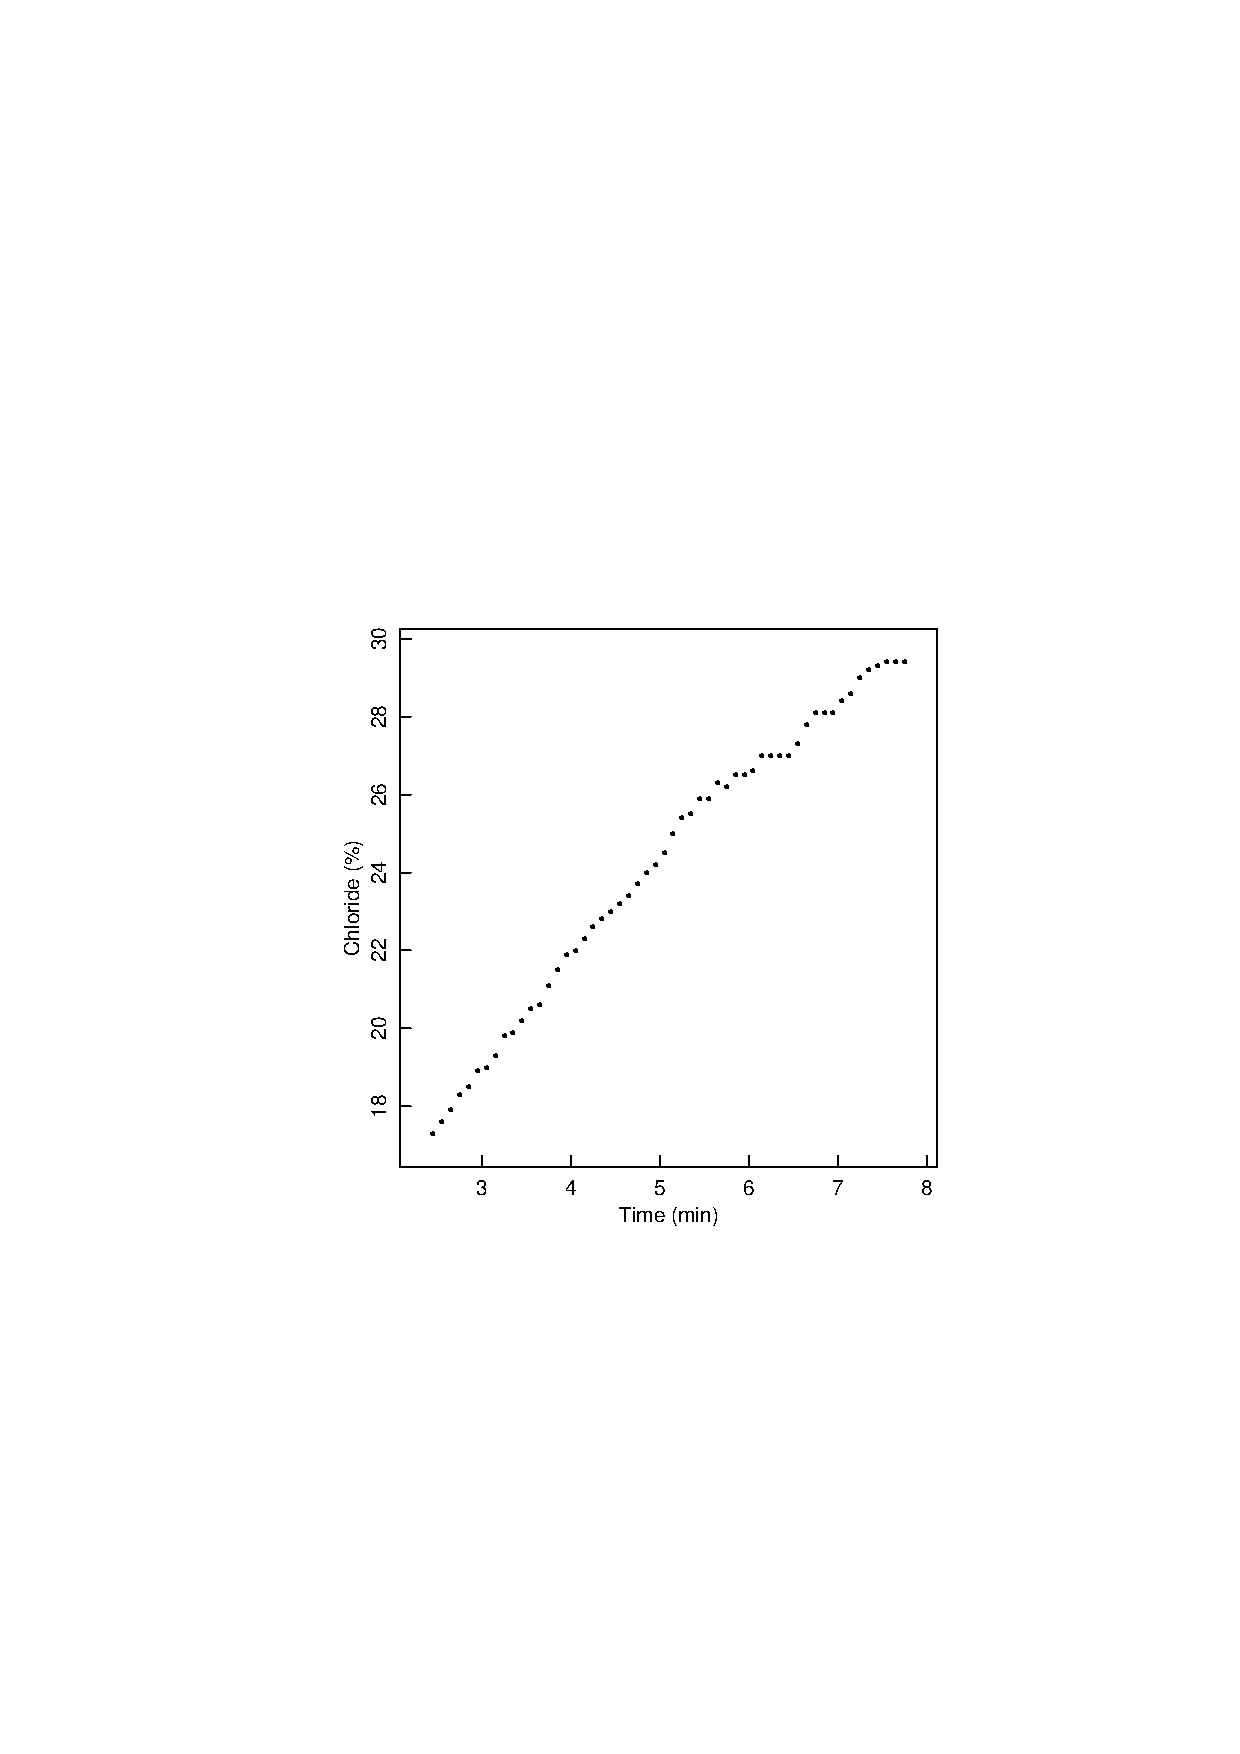
\includegraphics{3CHLdata}}%,height=3in}}
    \caption{Plot of chloride concentration versus time for the chloride
    transport data.}
    \label{fig:CHLdata}
  \end{figure}
The observation $y_{n}$ gives the chloride
concentration (in percent) at time $x_{n}$ (in minutes).

The model function
\begin{displaymath}
f ( x_n , \btheta ) = \theta_1
( 1 - \theta_2 e^{ - \theta_3 x_n } )
\end{displaymath}
was derived from the theory of ion transport,
where $\theta_{1}$ represents the final percentage
concentration of chlorine, $\theta_{3}$ is a rate constant,
and $\theta_{2}$ accounts for the
unknown initial and final concentrations of the chlorine and
the unknown initial reaction time.
As usual, it was assumed that the disturbances had zero mean and
constant variance and were independent.

An initial estimate for $\theta_{1}$ was obtained by
extrapolating the data to large time, giving
$\theta_1^0 = 35$.
Dividing $y_n $ by $\theta_1^{0}$ and linearizing
the equation by rearranging terms and taking logarithms
allowed us to estimate the remaining parameters by linear
regression, to give
$\btheta^0 = (35, 0.91, 0.22) \trans$.
Convergence was obtained to
$\hat{\btheta}= (39.09, 0.828,0.159)\trans$
with a residual sum of squares of 1.88.
\begin{figure}
  \vspace{2.25in}
  \centerline{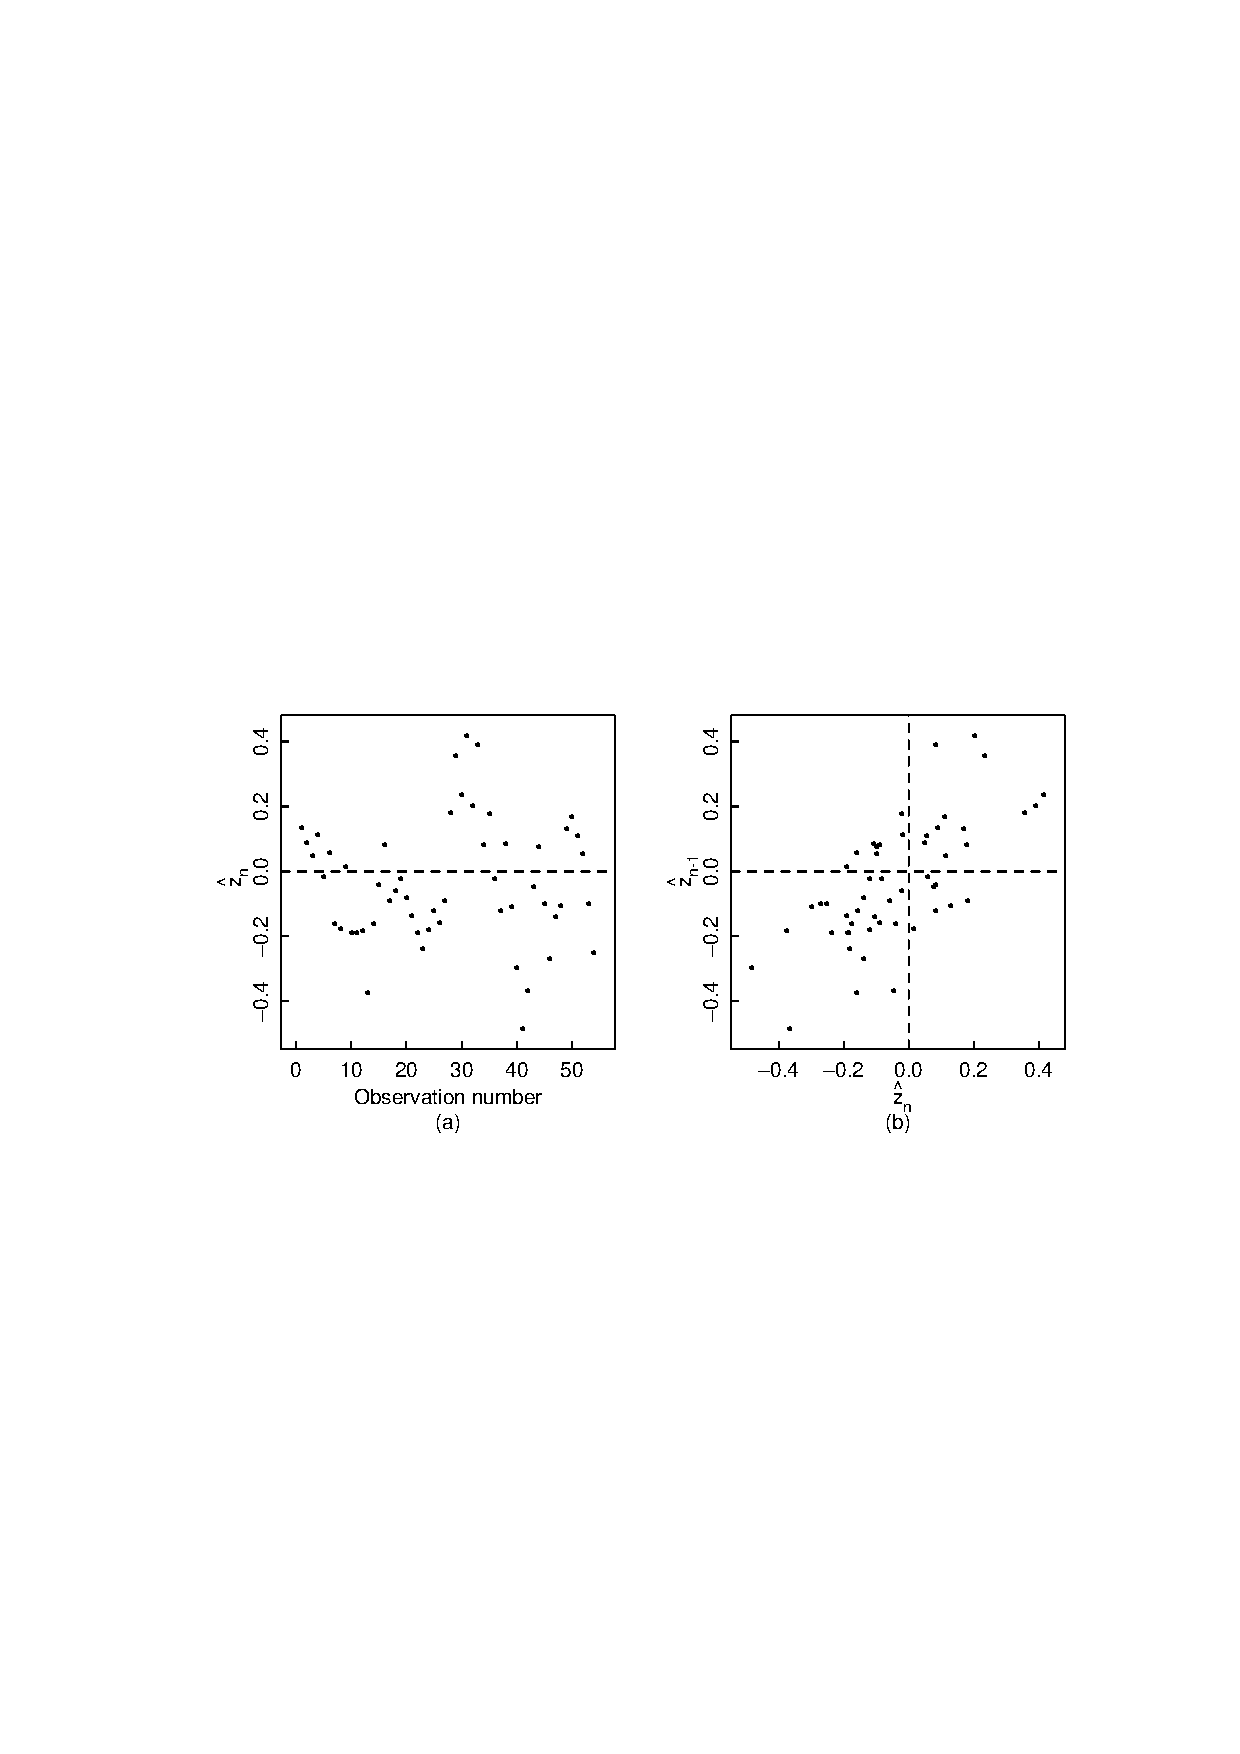
\includegraphics{3CHLres1}}%,height=2.25in}}
  \caption{Plots of the residuals $\hat z$ from the original nonlinear
    least squares fit to the chloride data.  The residuals are plotted
    as a time series in part $a$ and as a lag plot in part $b$.}
  \label{fig:CHLres1}
  \end{figure}
A time series plot of the residuals, shown in Figure~\ref{fig:CHLres1}$a$,
shows runs in the residuals.
Similarly, the lag plot shown in Figure~\ref{fig:CHLres1}$b$,
shows positive correlation.
We are thus alerted to the possibility that the disturbances are
not independent, or that there is some deficiency in the form of
the expectation function.
\end{example}

When the disturbances are not independent, the
model for the observations must be altered to account for
dependence.
Common forms for dependence, or \emph{autocorrelation}, of
\index{autocorrelation!of residuals}
disturbances are \emph{moving average}
or \emph{autoregressive}
\index{time series!moving average model}
\index{time series!autoregressive model}
models of variable order \cite{box:jenk:1976}.
%\glossary{ Box, G.E.P.}
%\glossary{ Jenkins, G.M.}
Simple examples of such forms are a moving average process of
order 1 where
\begin{displaymath}
Z_n = \epsilon_n - \omega_1 \epsilon_{n-1}
\end{displaymath}
or an autoregressive process of order 1 where
\begin{displaymath}
Z_n = \epsilon_n + \phi_1 Z_{n-1}
\end{displaymath}
and the $\epsilon_n , n = 1, 2 ,\ldots, N$, are independent random
disturbances with zero mean and constant variance,
or more simply, \emph{white noise}.

In regression situations,
when the data are equally spaced in time, it is relatively easy
to determine an appropriate form for the dependence of the
disturbances by calculating and plotting the \emph{residual
autocorrelation function},
\index{residual!autocorrelation function}
\begin{displaymath}
r_k = \sum_{n=k+1}^N
\frac{\hat z_n\hat z_{n-k}}{N s^2}   
k = 1,  2,\ldots
\end{displaymath}
versus the lag $k$.
In the definition of $r_{k}$, $s^{2}$ is the
variance estimate,
and the residuals are assumed to have zero average.
The residual autocorrelation function is usually calculated
out to $ k  \approx  N / 5 $.
If the residual autocorrelation function is consistently within
the range $\pm 2 / \sqrt N $ after lag 2 or 3, then
the model may be identified as a moving average process of order
1 or 2.
If the residual autocorrelation function tends to decay gradually
to zero, then the process may be identified as an autoregressive
process.
Alternatively, to determine the order of the autoregressive
process, it may be necessary to calculate the
\emph{partial autocorrelation function}
\cite{box:jenk:1976}.
%\glossary{ Box, G.E.P.}
%\glossary{ Jenkins, G.M.}
\index{partial autocorrelation function}
For regression situations where time is not the only
factor, or the most important factor, first order
autoregressive processes are often adequate.

\begin{example}\label{chlor:2}

The residual autocorrelation function for the chloride
  \begin{figure}
    \vspace{2.25in}
    \centerline{\includegraphics{3CHLauto}}%,height=2.25in}}
    \caption{
    Autocorrelation function of the residuals from the original nonlinear
    least squares fit to the chloride data.
    The dotted lines enclose the interval in which approximately 95\% of
    the correlations would be expected to lie if the true correlations
    were 0.
    }\label{fig:CHLauto}
  \end{figure}
data was calculated and plotted as in Figure \ref{fig:CHLauto}.
The correlation estimates decay towards zero, falling within
the limits $\pm 2 / \sqrt N$ (shown as dotted horizontal
lines) quite quickly.
On the basis of this plot, it was decided that a first order
autoregressive
process would adequately model the dependence in the residuals.

The model to be fitted is now of the form
$Y_n = f ( x_n , \btheta ) + Z_{n}$, where
$Z_n = \epsilon_n + \phi  Z_{n-1}$.
To estimate the parameters $\btheta$ and $\phi$, we
reduce the problem to an ordinary nonlinear least
squares problem by subtracting $\phi$ times the equation for
$Y_{n-1}$ from $Y_{n}$, as
\begin{displaymath}
Y_n - \phi Y_{n-1} =
f ( x_n , \btheta ) - \phi 
f ( x_{n-1} , \btheta ) + Z_n - \phi  Z_{n-1}
\end{displaymath}
or
\begin{displaymath}
Y_n = \phi Y_{n-1} +
f ( x_n , \btheta ) - \phi  f ( x_{n-1} , \btheta ) + \epsilon_n
\end{displaymath}

Starting values for $\btheta$ were taken from $\hat{\btheta}$
above, and the starting value for $\phi$ was taken as the lag
one correlation estimate, $r_1 = 0.67$.
Convergence was obtained to
$( \btheta \trans , \phi ) = ( 37.58,  0.849,  0.178,  0.69 )$
with a residual sum of squares of 0.98.
The residuals $\hat \epsilon$ from this fit are
\begin{figure}
  \centerline{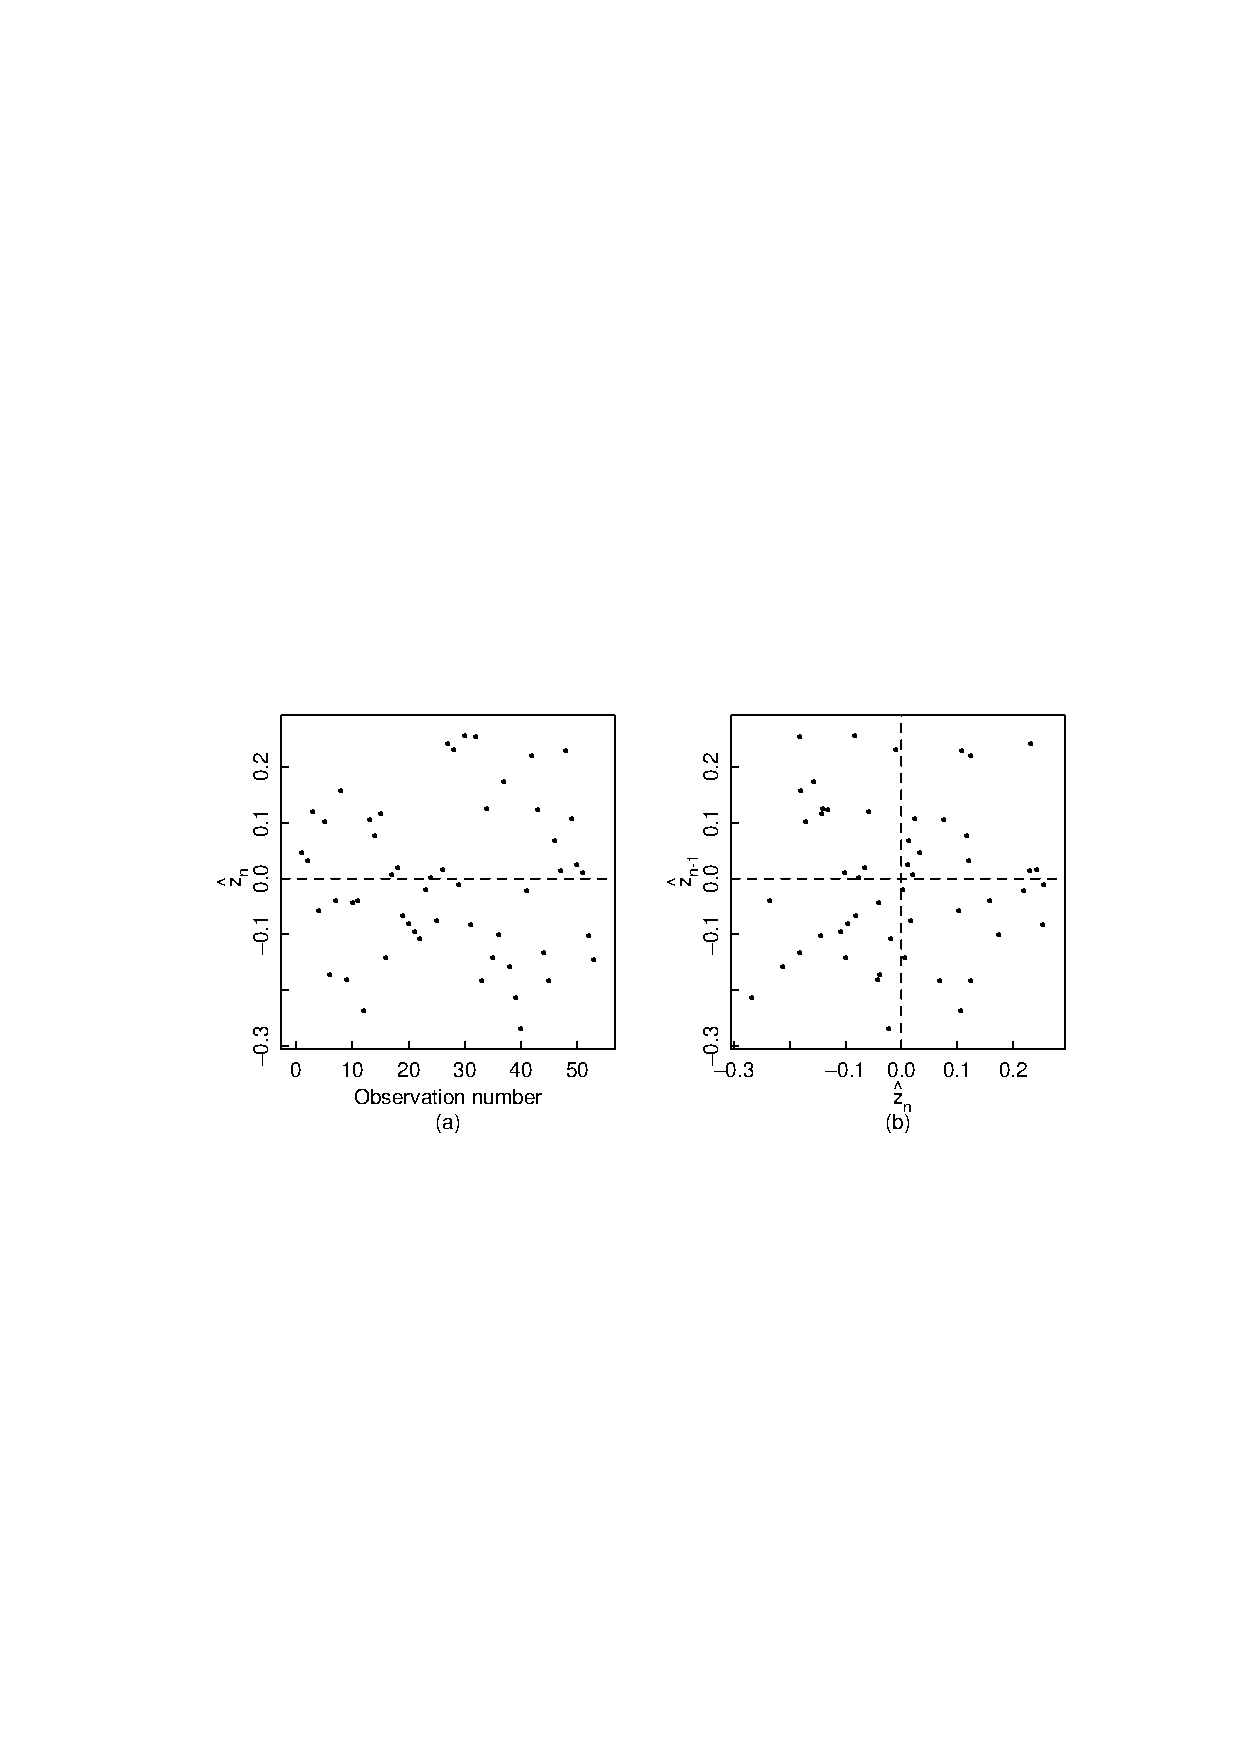
\includegraphics{3CHLres2}}%,height=2.25in}}
  \caption{Plots of the residuals $\hat z$ from the nonlinear least
    squares fit to the chloride data using $\phi=0.69$.  The residuals
    are plotted as a time series in part $a$ and as a lag plot in part
    $b$.}
  \label{fig:CHLres2}
\end{figure}
well behaved, as shown in Figure \ref{fig:CHLres2} and
\begin{figure}
  \centerline{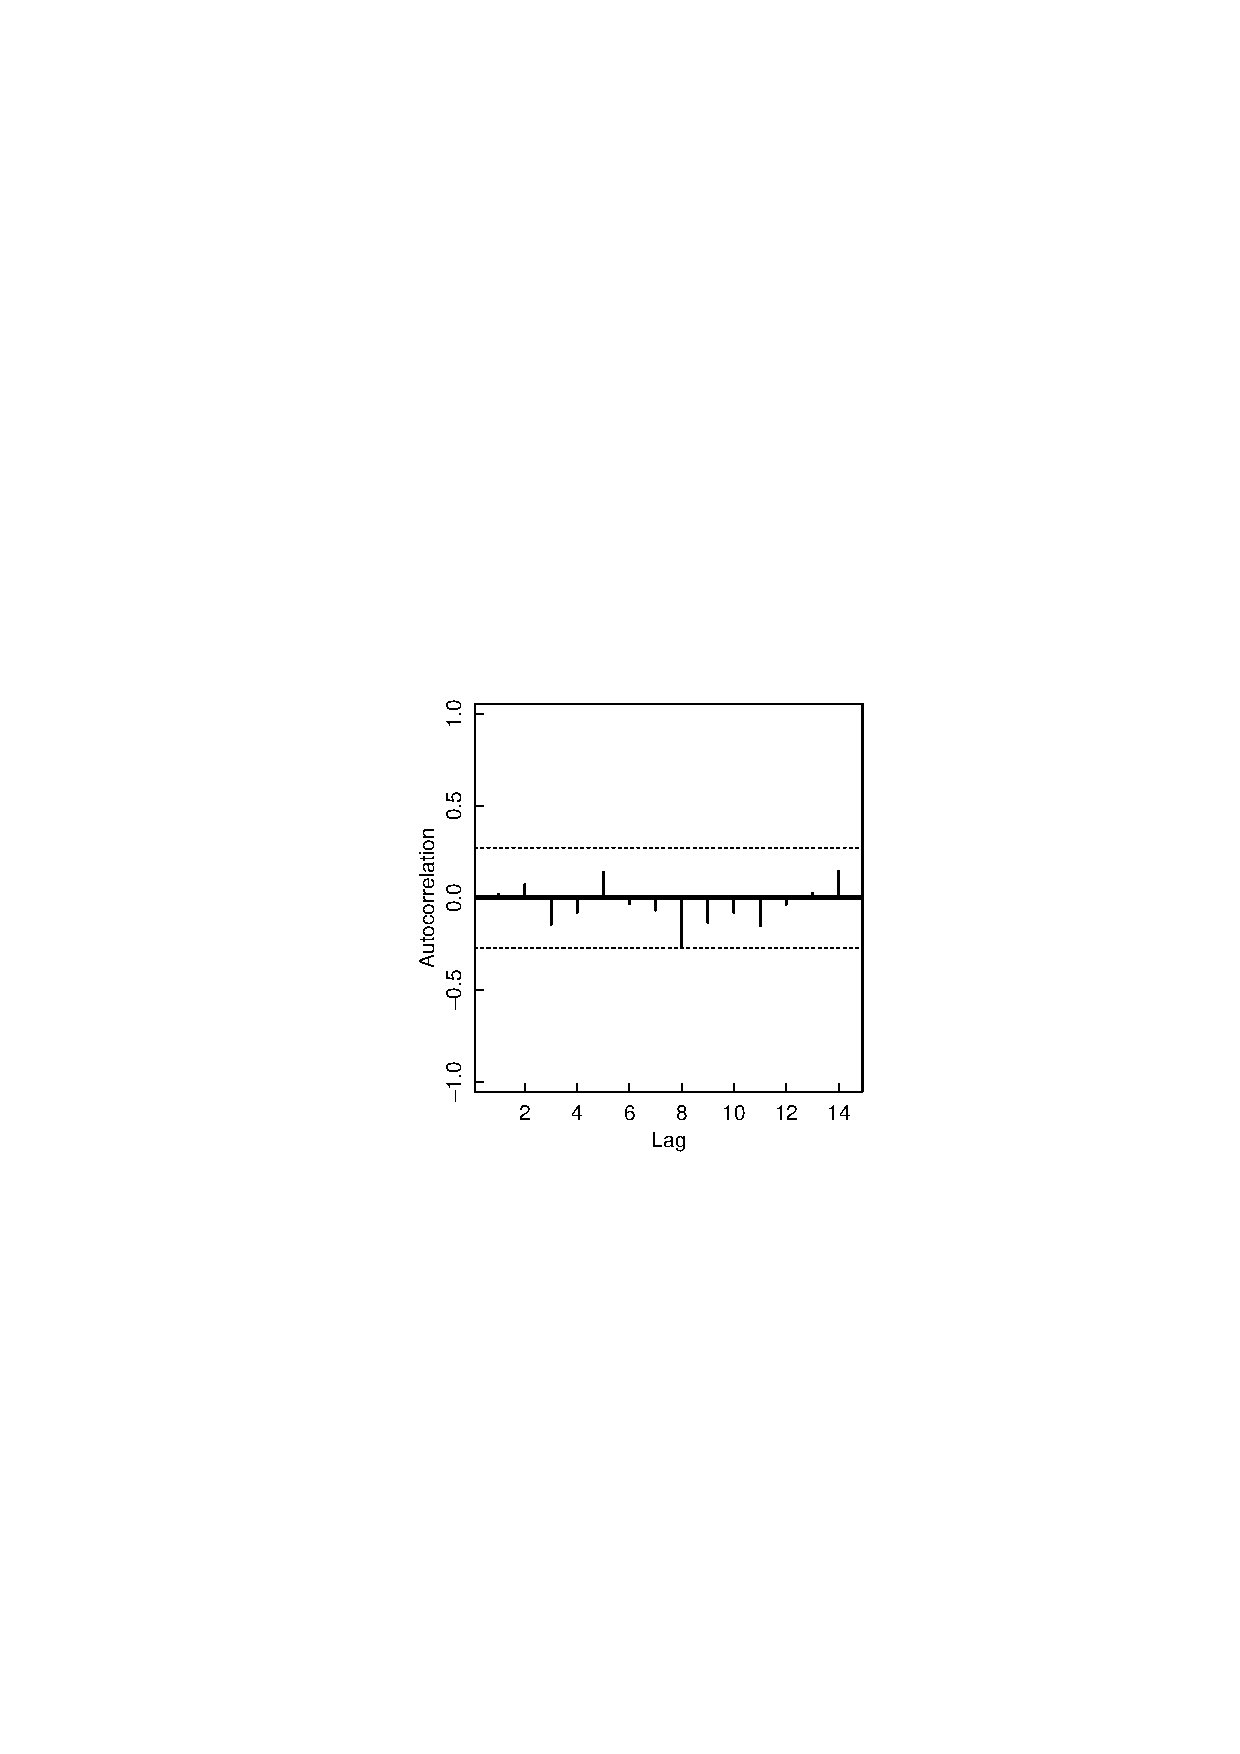
\includegraphics{3CHLacf2}}%,height=2.25in}}
  \caption{Autocorrelation function of the residuals from the nonlinear
    least squares fit to the chloride data using $\phi=0.69$.  The
    dotted lines enclose the interval in which approximately 95\% of
    the correlations would be expected to lie if the true correlations
    were 0.}
  \label{fig:CHLacf2}
  \end{figure}
the residual autocorrelation function, shown in Figure
\ref{fig:CHLacf2}, was uniformly small.
\end{example}

In general, as in the above example,
the main effect of accounting for dependence is to
reduce the residual variance and reduce the correlation in
the residuals: the model parameter estimate
$\hat{\btheta}$ does not change much.
However, the model parameters are better estimated
because they have smaller standard errors and because the
method of least squares has been applied correctly,
since the assumptions are satisfied.
For a more complicated application of this technique, see
\citeasnoun{watt:baco:1974}.
%\glossary{ Watts, D.G.}
%\glossary{ Bacon, D.W.}

\section{Accumulated Data}
\index{practical considerations!accumulated data}
\index{accumulated data}

In some studies, when it is impractical to measure instantaneous
concentrations, \emph{accumulated}
responses are recorded.
\label{eth:1}
\begin{example}

An experiment to study the metabolism of ethyl acrylate was
performed by giving rats a single bolus of radioactively tagged
ethyl acrylate.
Each rat was given a measured dose of the compound via stomach
intubation and placed in an enclosed cage from which the air
could be drawn through a bubble chamber.
The exhaled air was bubbled through the chamber, and at a
specified time the bubble chamber was replaced by a fresh one, so
that the measured response was the accumulated CO$_{2}$ during
the time interval.
Preliminary analysis of the data revealed that normalizing each
animal's response by dividing by the actual dose received would
permit combination of the data so that a single model could be
fitted to the data for all the rats.
Furthermore, the variability in the normalized data was such that
it was necessary to take logarithms of the data to produce
constant variance across the time points.
The starting points and lengths of the accumulation intervals and the
averages for the nine rats, normalized by actual dose, are given
in Appendix~\ref{atbl:co2} \cite{watt:debe:stir:1986}, and
%\glossary{ Watts, D.G.}
%\glossary{ deBethizy, D.}
%\glossary{ Stiratelli, R.G.}
the cumulative CO$_{2}$ data are plotted
in Figure \ref{fig:CO2data}.
\begin{figure}
  \centerline{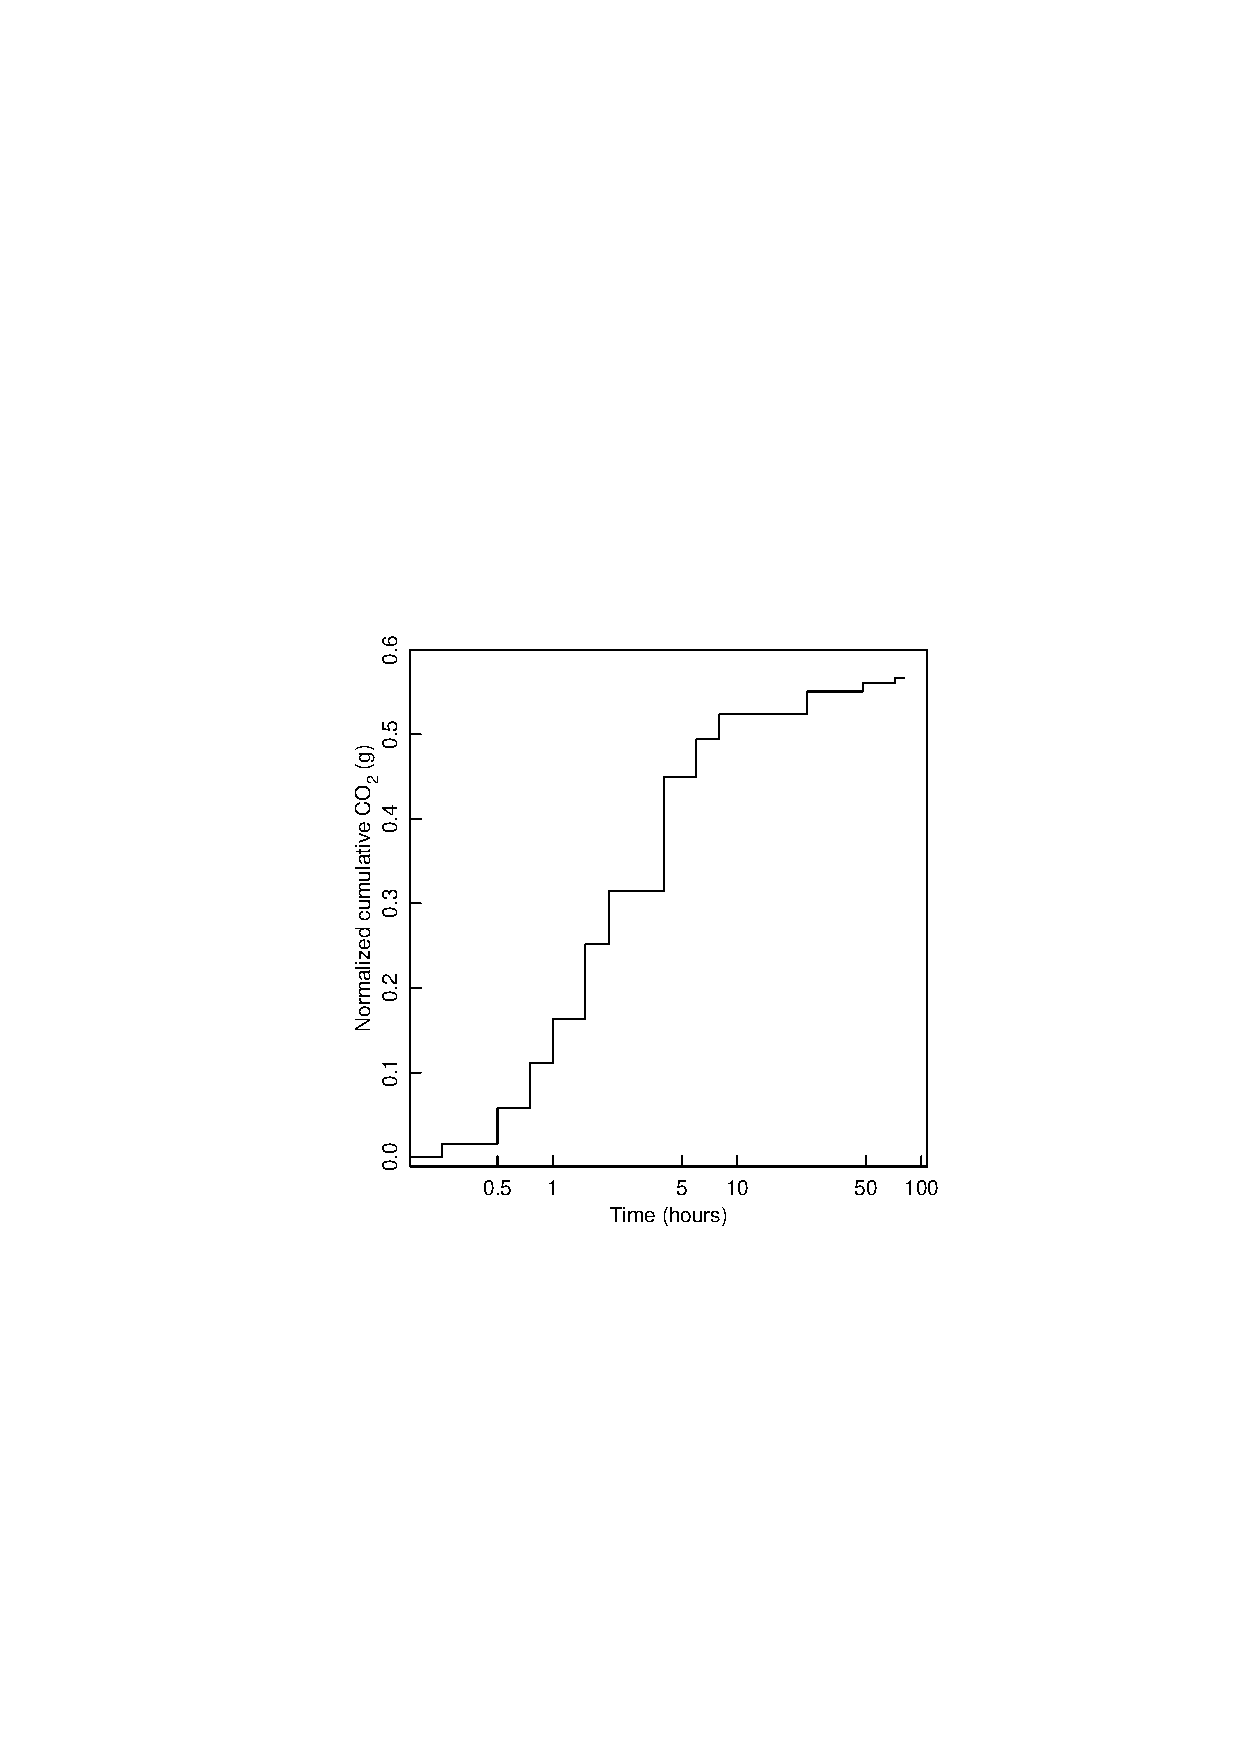
\includegraphics{3CO2data}}%,height=3in}}
  \caption{Plot of cumulative exhaled CO$_{2}$ amounts versus
    collection interval end point for the ethyl acrylate data.}
  \label{fig:CO2data}
  \end{figure}
\end{example}

Two methods for the analysis of such data were given in \citeasnoun{renw:1982}.
%\glossary{ Renwick, A.G.}
The first method uses peeling of the ``approximate concentration''
data obtained by dividing the accumulated amount by
the accumulation time interval.
The second method
uses the cumulative total, extrapolated to infinite time,
and then peeling of the differences
\index{peeling}
$[ extrapolated - (cumulative  total)]$.
This is called the ``sigma-minus''
\index{sigma-minus method!for accumulated data}
method.

We do not recommend either of these methods, and specifically
decry use of the sigma--minus method because it is so sensitive
to variations in the extrapolated value.
It can be shown, for example, that small percentage changes in the
extrapolated value, say less than 2\%, can cause
changes in the rate constants in excess of 100\%.
Furthermore, both methods are based on peeling, which requires
excessive subjective judgement.
Instead of the abovementioned methods, we recommend direct
analysis of the accumulated data using integrated responses
as described below.
In addition to avoiding the disadvantages of the other methods, this
method has the advantage that it provides measures of precision of the
estimates in the form of parameter approximate standard errors and
correlations.

\subsection{Estimating the Parameters by Direct Integration}
\index{accumulated data!analysis by direct integration}

Suppose that the theoretical response to the input stimulus at time
$t$ is $f ( t, \btheta )$.
Then the accumulated output in the interval
$t_{n-1}$ to $t_{n}$ is
\begin{displaymath}
F_n =
\int_{t_{n-1}}^{t_n} f(t,\btheta) dt
\end{displaymath}
We therefore use the integrated function values $F_n $ and the observed
accumulated data pairs $( y_n ,t_n )$ to estimate the
parameters.
We rewrite the model in terms of the factors $x_{1n}=t_{n-1}$,
the start of the interval, and $x_{2n}=t_n-t_{n-1}$, the
length of the interval, so the model for the amount accumulated in an
interval is $F(\bx_n,\btheta)$, where
$\bx_n=(x_{1n},x_{2n})\trans$.

To determine a tentative form for $f ( t , \btheta )$, we plot the
approximate rates
${y_n} / {x_{2n}}$ versus
$x_{1n}+x_{2n} / 2$ on semilog paper and use peeling to
obtain \emph{starting} estimates for the parameters.
The final estimation is done using nonlinear least squares.
Note that if the variance is not constant, it may be necessary to
transform the data and the function, as in the following example.

\begin{example}\label{eth:2}
  The CO$_{2}$ data are reproduced in Table~\ref{tbl:CO2rate} together
  with the derived quantities (interval midpoint
  $x_{1n}+ x_{2n} / 2$ and approximate rate
  $y_n / x_{2n}$) which are plotted in Figure~\ref{fig:CO2apconc}.
  \begin{table}
    \caption{
      Collection intervals and averages of normalized exhaled CO$_{2}$
      for the ethyl acrylate data together with the derived quantities:
      interval midpoint and approximate rate }\label{tbl:CO2rate}
    \begin{center}
      \begin{tabular}{cclll} \hline
        \multicolumn{2}{c}{Collection} & &
        \multicolumn{2}{c}{Derived}\\ \multicolumn{2}{c}{Interval (hr)} &
        & \multicolumn{2}{c}{Quantities}\\ \multicolumn{1}{c}{Start} &
        \multicolumn{1}{c}{Length} & \multicolumn{1}{c}{CO$_{2}$} &
        \multicolumn{1}{c}{Interval} & \multicolumn{1}{c}{Approx.}\\
        \multicolumn{1}{c}{$x_{1}$} & {$x_{2}$} & \multicolumn{1}{c}{(g)}
        & \multicolumn{1}{c}{Midpoint} & \multicolumn{1}{c}{Rate}\\ \hline
        0.0&0.25&0.01563&0.125&0.0625\\ 0.25&0.25&0.04190&0.375&0.1676\\
        0.5&0.25&0.05328&0.625&0.2131\\ 0.75&0.25&0.05226&0.875&0.2090\\
        1.0&0.5&0.08850&1.25&0.1770\\ 1.5&0.5&0.06340&1.75&0.1268\\
        2.0&2.0&0.13419&3.0&0.0671\\ 4.0&2.0&0.04502&5.0&0.0225\\
        6.0&2.0&0.02942&7.0&0.0147\\ 8.0&16.0&0.02716&16.0&0.0017\\
        24.0&24.0&0.01037&36.0&0.0004\\ 48.0&24.0&0.00602&60.0&0.0003\\
        \hline
      \end{tabular}
    \end{center}
  \end{table}
  \begin{figure}
    \centerline{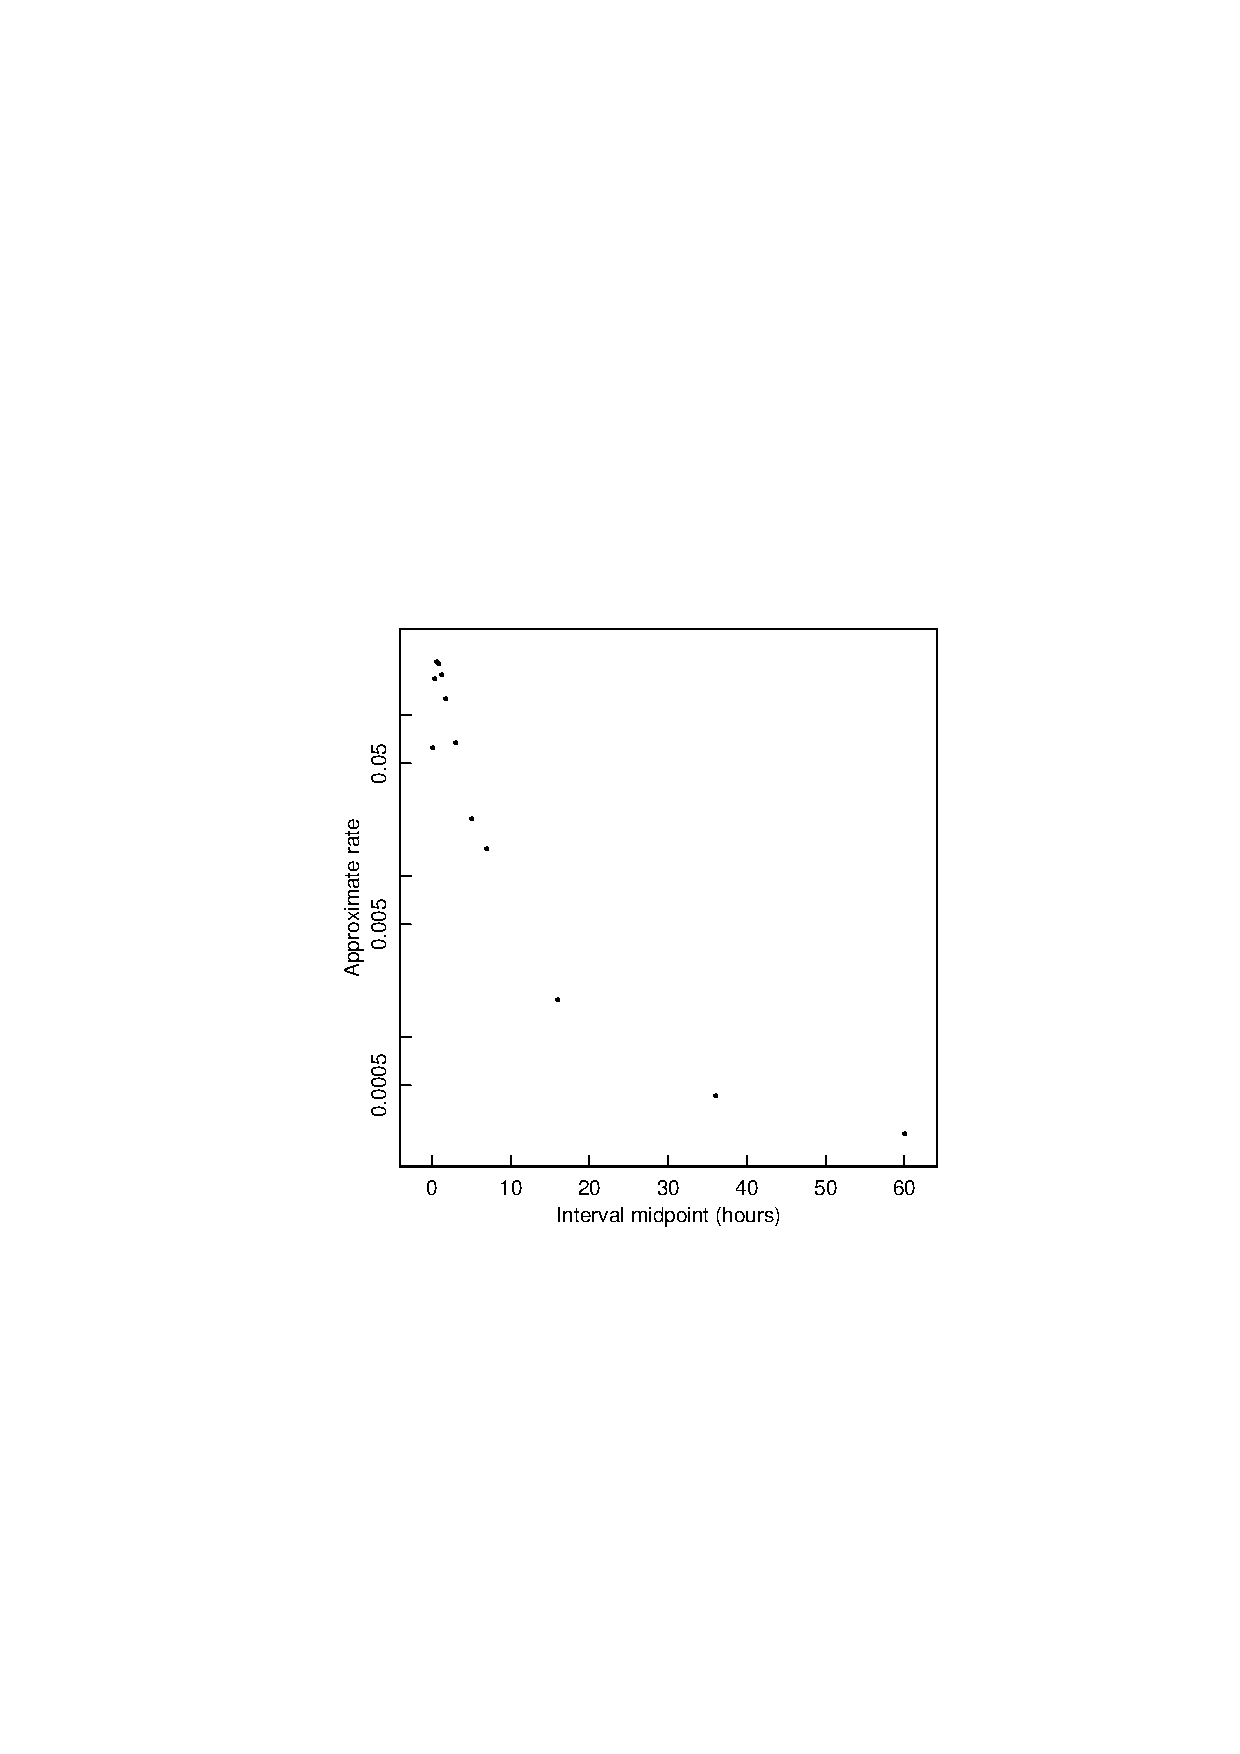
\includegraphics{3CO2apconc}}%,height=3in}}
    \caption{Approximate CO$_{2}$ exhalation rate versus collection
      interval midpoint for the ethyl acrylate data.}
    \label{fig:CO2apconc}
  \end{figure}
  We can see from the figure that an
  appropriate model for the data involves three exponentials
  (two to account for the peak, and another to account for the
  change in slope of the decay from the peak).
  Because the radioactivity prior to injection must be zero,
  the concentration at $ t = 0$ must be zero.
  A plausible model for the concentration at time $t$ is therefore
  \begin{displaymath}
    f(t, \btheta )=- ( \theta_4 + \theta_5 ) e^{ - \theta_1 t }
    + \theta_4 e^{{-} \theta_2 t }
    + \theta_5 e^{{-} \theta_3 t }
  \end{displaymath}
  An appropriate model for the accumulated data in the
  collection interval starting at $t_{n-1} $ is then
  \begin{eqnarray*}
    F_n&=&-\frac{\theta_4+\theta_5}{\theta_1}( e^{ - \theta_1 t_{n-1} } -
    e^{ - \theta_1 t_n } )\\
    &&+\frac{\theta_4}{\theta_2}(e^{-\theta_2 t_{n-1} }-e^{-\theta_2 t_n})
    +\frac{\theta_5}{\theta_3}
    ( e^{{-} \theta_3 t_{n-1} } - e^{{-} \theta_3 t_n} )
  \end{eqnarray*}
  or
  \begin{eqnarray*}
    F(\bx,\btheta)&=&
    -\frac{\theta_4+\theta_5}{\theta_1}e^{-\theta_1 x_1}(1-e^{-\theta_1 x_2})\\
    &&+\frac{\theta_4}{\theta_2}e^{-\theta_2 x_1}(1-e^{-\theta_2 x_2})
    +\frac{\theta_5}{\theta_3}e^{-\theta_3 x_1}(1-e^{-\theta_3 x_2})
  \end{eqnarray*}
  Because of the nonconstant variance, the logarithms of $F$ were
  fitted to the logarithms of the data.
  The results of this analysis together with the starting estimates
  are presented
  in Table~\ref{tbl:5.2}.
  \begin{table}
    \caption{
      Parameter summary for the 3-exponential model fitted to the
      ethyl acrylate data.}\label{tbl:5.2}
    \begin{center}
      \begin{tabular}{cllc}\hline
        & & \multicolumn{2}{c}{Nonlinear Least Squares}\\ & & &
        \multicolumn{1}{c}{Approx.}\\ \multicolumn{1}{c}{Parameter} &
        \multicolumn{1}{c}{Start} & \multicolumn{1}{c}{Estimate} &
        \multicolumn{1}{c}{Std. Err.}\\ \hline
        $\theta_{1}$&4.461&3.025&0.752\\ $\theta_{2}$&0.571&0.481&0.038\\
        $\theta_{3}$&0.0434&0.0258&0.0096\\ $\theta_{4}$&0.355&0.310&0.049\\
        $\theta_{5}$&0.0034&0.0011&0.0005\\ \hline
      \end{tabular}
    \end{center}
  \end{table}
  In an analysis of the logarithmic data for the individual rats, due
  attention was paid to the behavior of the residuals.
  The triple rate constant model fitted the data very well.
\end{example}

\begin{example}\label{sac:1}
  As a second example of treating accumulated data,
  we analyze the saccharin data in \citeasnoun{renw:1982}.
  % \glossary{ Renwick, A.G.}
  In this experiment, the measured response was the amount of
  saccharin accumulated in the urine of a rat after receiving a
  single bolus of saccharin.
  The data are recorded in Appendix~\ref{atbl:sac}, and plotted
  in Figure~\ref{fig:SACdata}.
  \begin{figure}
    \centerline{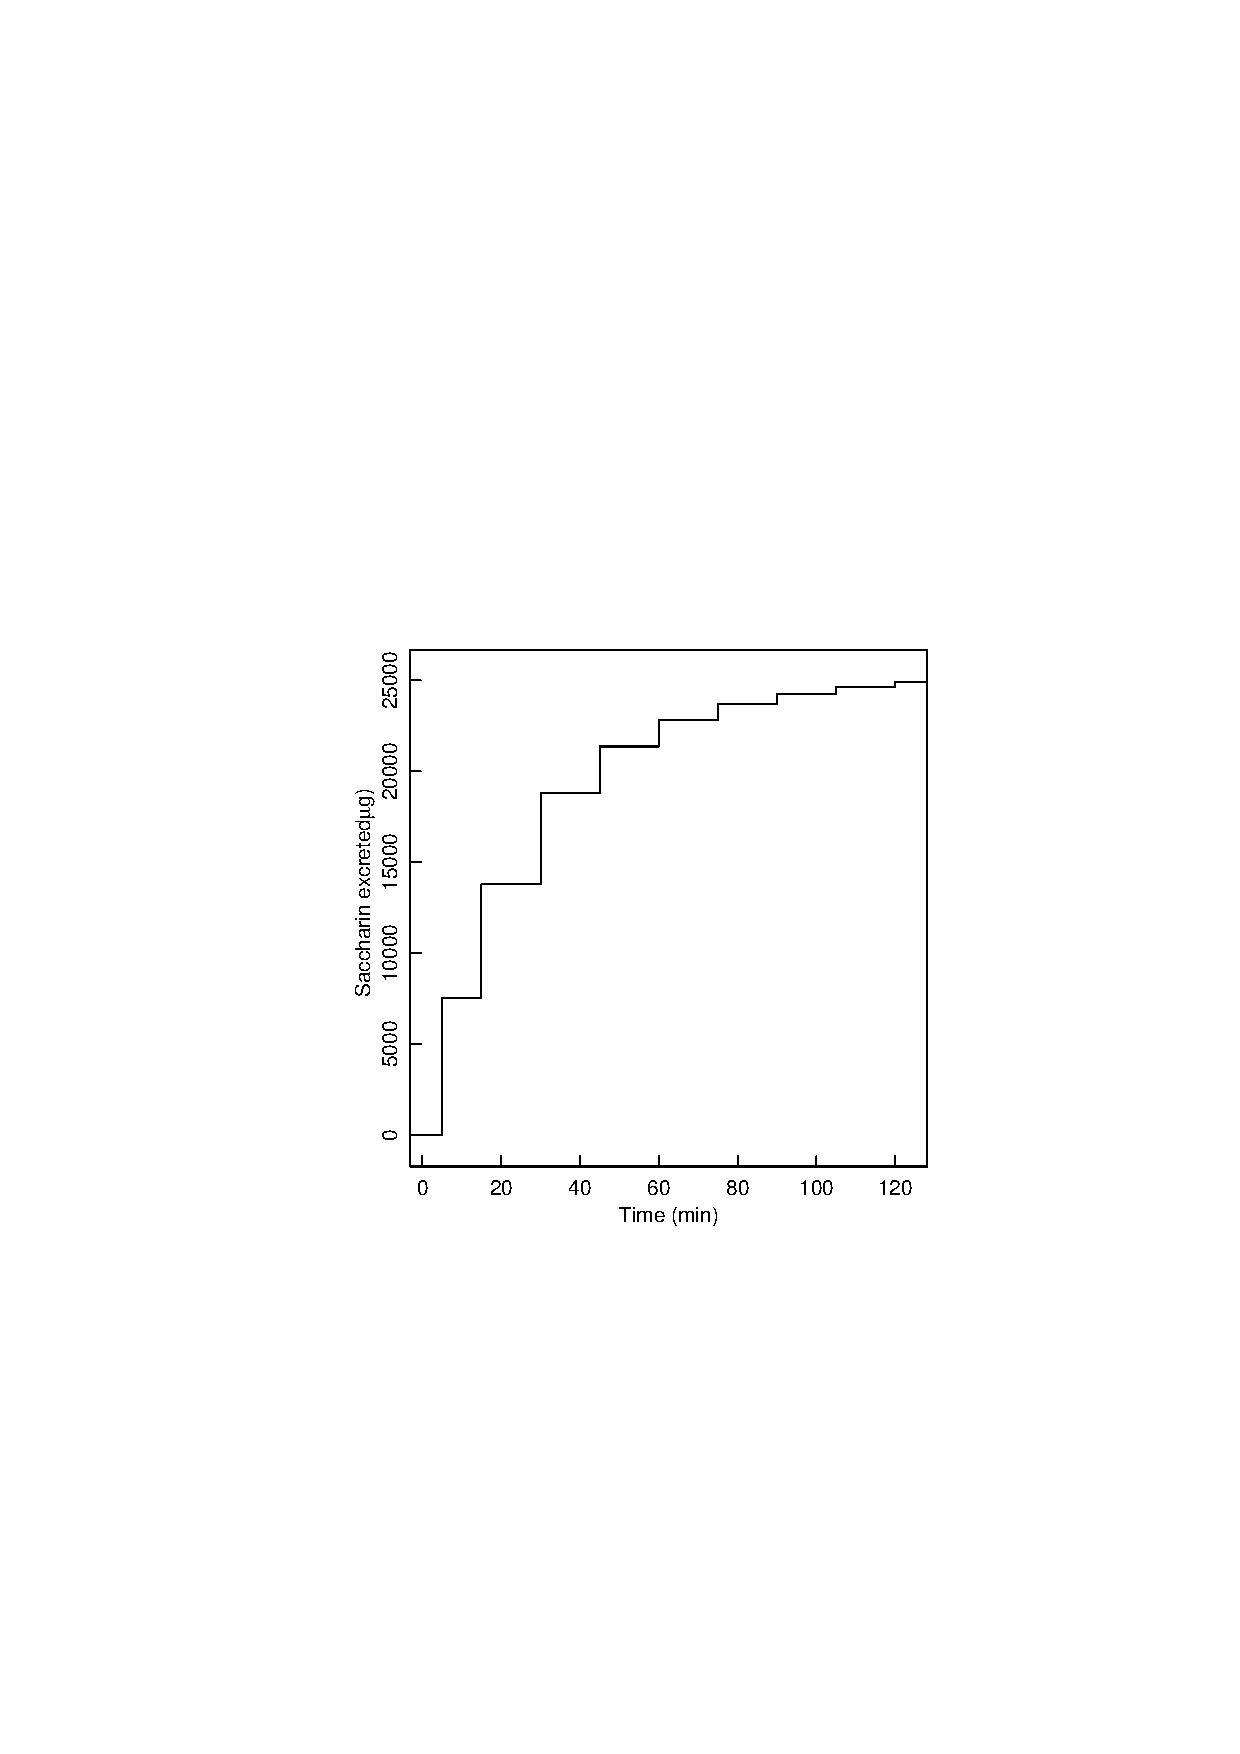
\includegraphics{3SACdata}}%,height=3in}}
    \caption{Plot of cumulative excreted amount versus collection
      interval end point for the saccharin data.}
    \label{fig:SACdata}
  \end{figure}
  
  The function involved only two rate constants, and the
  response was modeled as
  \begin{displaymath}
    f(t, \btheta ) = \theta_3 e^{ - \theta_1 t }
    + \theta_4 e^{{-} \theta_2 t }
  \end{displaymath}
  so
  \begin{displaymath}
    F(\bx,\btheta)=\frac{\theta_3}{\theta_1}e^{-\theta_1 x_1}
    ( 1 - e^{ - \theta_1 x_2} )
    +\frac{\theta_4}{\theta_2}
    e^{ - \theta_2 x_1 }
    ( 1 - e^{ - \theta_2 x_2} )
  \end{displaymath}
  As in the ethyl acrylate example, the integrated model was fitted to
  the logarithms of the accumulated data to stabilize
  variance.
  
  The curve peeling and the sigma--minus method results from \citeasnoun{renw:1982}
  % \glossary{ Renwick, A.G.}
  are given in columns 2 and 3 of
  Table \ref{tbl:3}, and the
  results using the direct integration method are given in column 4.
  \begin{table}
    \caption{
      Parameter summary for the saccharin data, comparing estimates
      obtained using the sigma--minus method, using the approximate rate
      method, and using nonlinear least squares to fit the integrated
      response function.  }\label{tbl:3}
    \begin{center}
      \begin{tabular}{clclc} \hline
        \multicolumn{5}{c}{Estimate by}\\ & & &
        \multicolumn{2}{c}{Nonlinear Least Squares}\\ & & & &
        \multicolumn{1}{c}{Approx.}\\ \multicolumn{1}{c}{Parameter} &
        \multicolumn{1}{c}{Peeling$^{a}$} &
        \multicolumn{1}{c}{Sigma--Minus$^{a}$} & \multicolumn{1}{c}{Value}
        & \multicolumn{1}{c}{Std. Err.}\\ \hline
        $\theta_{1}$&0.0710&0.0833&0.122&0.031\\
        $\theta_{2}$&0.0234&0.0255&0.0279&0.003\\
        $\theta_{3}$&830&932&1345&249\\
        $\theta_{4}$&270&314&402&98\\
        \hline
      \end{tabular}
    \end{center}
     $^{a}$ From \citeasnoun{renw:1982}.
%\glossary{ Renwick, A.G.}
   \end{table}
  
  Note the considerable differences between the results based on
  peeling and those obtained by nonlinear least squares.
  Note too, that the peeling and sigma--minus methods do not
  provide parameter standard errors.
  
  There were two very large residuals from the nonlinear least
  squares fit, at $x_1=5$ and $x_1=105$.
  A second analysis was done by simply combining the observations
  at $x_1=5$ and  $x_1=15$ and at
  $x_1=90$ and $x_1=105$, as shown in Table \ref{tbl:SACHed}.
  \begin{table}
    \caption{
      Collection intervals and excreted amounts for original and
      combined saccharin data.  }\label{tbl:SACHed}
    \begin{center}
      \begin{tabular}{cccccc} \hline
        \multicolumn{3}{c}{Original} & \multicolumn{3}{c}{Combined}\\
        \hline \multicolumn{2}{c}{Collection} & &
        \multicolumn{2}{c}{Collection} &\\ \multicolumn{2}{c}{Interval (hr)}
        & & \multicolumn{2}{c}{Interval (hr)} & \\ \multicolumn{1}{c}{Start}
        & \multicolumn{1}{c}{Length} & \multicolumn{1}{c}{Saccharin} &
        \multicolumn{1}{c}{Start} & \multicolumn{1}{c}{Length} &
        \multicolumn{1}{c}{Saccharin}\\ \multicolumn{1}{c}{$x_{1}$} &
        \multicolumn{1}{c}{$x_{2}$} & \multicolumn{1}{c}{$(\mu$g)} &
        \multicolumn{1}{c}{$x_{1}$} & \multicolumn{1}{c}{$x_{2}$} &
        \multicolumn{1}{c}{$(\mu$g)}\\ \hline 0&5&7518&0&5&7518\\
        5&10&6275&5&25&11264\\ 15&15&4989&\\ 30&15&2580&30&15&2580\\
        45&15&1485&45&15&1485\\ 60&15&861&60&15&861\\ 75&15&561&75&15&561\\
        90&15&363&90&30&663\\ 105&15&300\\ \hline
      \end{tabular}
    \end{center}
  \end{table}
  
  The residuals from this fit were very well behaved, and the
  residual variance was reduced to 0.0071 from 0.0158.
  The parameter estimates (standard errors in parentheses) were
  $\theta_1 = 0.154 (0.035)$,
  $\theta_2 = 0.030 (0.002)$,
  $\theta_3 = 1506  (233)$, and
  $\theta_4 =  472 (70)$.
\end{example}

\section{Comparing Models}
\index{practical considerations!comparing models}

In some situations there may be more than one function
which could be used as a model.
For example, in fitting a double exponential model,
\begin{displaymath}
  f ( x , \btheta ) = \theta_1 e^{ - \theta_2 x } +
  \theta_3 e^{ - \theta_4 x}
\end{displaymath}
$\theta_{4}$ could be $0$, in which case the model reduces to
\begin{displaymath}
  f ( x , \btheta ) = \theta_1 e^{ - \theta_2 x } + \theta_3
\end{displaymath}
or $\theta_{3}$ could be 0, in which case the model reduces to
\begin{displaymath}
  f ( x , \btheta ) = \theta_1 e^{ - \theta_2 x }
\end{displaymath}
In this situation of \emph{nested} models, we would be
\index{nested model}
\index{model!nested}
interested in finding the simplest model which adequately fits the data.

In other situations, we might compare \emph{non-nested}
\index{model!non-nested}
models---for example, model 1
\begin{displaymath}
  f ( x , \btheta ) = \theta_1 ( 1 - e^{ - \theta_2 x } )
\end{displaymath}
versus model 2
\begin{displaymath}
  f ( x , \btheta )=\frac{\theta_1x}{\theta_2+x}
\end{displaymath}
both of which start at $f=0$ when $x=0$ and approach the
asymptote $\theta_{1}$ as $x\to\infty$.
In these situations, one model may give a superior fit to the data,
and we would like to select that model.

\subsection{Nested Models}

To decide which is the simplest nested model to fit a
data set adequately, we proceed as in the linear case and use
a likelihood ratio test \cite{drap:smit:1998}.
Because of the spherical normal assumption, this leads to an
assessment of the extra sum of squares
\index{extra sum of squares!analysis for nested models}
\index{sum of squares!extra}
due to the extra parameters involved in
\index{parameter!extra degrees of freedom}
\index{degrees of freedom!extra parameter}
going from the partial to the full model.

Letting $S$ denote the sum of squares, $\nu$ the degrees of
freedom, and $P$ the number of parameters, with subscripts $f$
and $p$ for the \emph{full}
and \emph{partial} models and a subscript $e$
for \emph{extra},
the calculations can be summarized as in
Table~\ref{tbl:extra}.
\begin{table}
  \caption{Extra sum of squares analysis for nested models.}
  \label{tbl:extra}
  \begin{center}
    \begin{tabular}{c  c  c  c  c} \hline
      & \multicolumn{1}{c}{Sum of} & \multicolumn{1}{c}{Degrees of}
      &\multicolumn{1}{c}{Mean Square} & \multicolumn{1}{c}{F Ratio}\\
      \multicolumn{1}{c}{Source} & \multicolumn{1}{c}{Squares}
      &\multicolumn{1}{c}{Freedom} \\ \hline Extra parameters&$S_e = S_p -
      S_{f}$& $\nu_e = P_f - P_{p}$&$s_e^2 = S_e / \nu_{e}$&
      ${s_e^2}/{s_f^2}$\\ Full model&$S_{f}$&$\nu_f = N - P_{f}$& $s_f^2 =
      S_f / \nu_{f}$\\ \hline Partial model&$S_{p}$&$N - P_{p}$\\ \hline
    \end{tabular}
  \end{center}
\end{table}
To complete the analysis, we compare the ratio $s_e^2 / s_f^{2}$ to
$F(\nu_e,\nu_f;\alpha)$ and accept the 
partial model if the calculated mean square ratio is lower than the
table value.
Otherwise, we retain the extra terms and use the full model.
Illustrations of the use of the extra sum of squares analysis are
given below in Example Puromycin~\ref{mic:10} and in Section 3.11.

Note that for linear least squares, the extra sum of squares
analysis is exact because the
data vector $\by$ is being projected onto linear subspaces of the
response space to determine $S_{p}$ and $S_{f}$.
Mathematically, the partial model
expectation plane is a linear subspace of the full model
expectation plane.
Residual vectors can then be decomposed into orthogonal
components and, from the fact that the full model residual vector
has a squared length which is distributed as a
$\sigma^2 \chi^{2}$ random variable with $N - P$ degrees of
freedom, it follows that the squared lengths of the components
are also distributed as $\sigma^2 \chi^{2}$ random variables
with degrees of freedom equal to the dimensions of the linear
subspaces.

For nonlinear models, as we might expect, the analysis is only
approximate because the calculated mean square ratio will not have
an exact F distribution.
However, the distribution of the mean square ratio is only
affected by intrinsic nonlinearity and not by parameter effects
nonlinearity,
\index{extra sum of squares!and nonlinearity}
and, as shown in Chapter 7, the intrinsic nonlinearity is generally small.
When the partial model is inadequate,
the effect of intrinsic nonlinearity on the analysis can be large but the
partial model will be rejected anyway:
it is only when the fitted values are very close that the form of the
distribution is critical.
In these cases, the intrinsic nonlinearity will usually
have a small effect because the expected responses being compared are close
together on the expectation surface.
\subsection{Incremental Parameters and Indicator Variables}

Many nested models can be parametrized in terms of incremental
parameters.
An \emph{incremental parameter} accounts for a
\index{parameter!incremental}
\index{incremental!parameter}
change in a parameter between blocks of cases and is
associated with an indicator variable.
\index{indicator variable}
\index{variable!indicator}
An advantage of using incremental parameters is that a
preliminary evaluation of the need for the full model can
be made directly from the regression output without having
to do additional computation.
The use of incremental parameters is most easily described by
means of an example.

\begin{example}
  \label{mic:10}
  In the Puromycin experiment, two blocks of experiments were run.
  In one the enzyme was treated with puromycin (Table A1.3$a$), and
  in the other the same enzyme was untreated
  (Table A1.3$b$).
  It was hypothesized that the Puromycin should affect the maximum
  velocity parameter $\theta_{1}$, but not the half-velocity
  parameter $\theta_{2}$.
  The two data sets are plotted in
  Figure~\ref{fig:MIC2data}.
  \begin{figure}
    \centerline{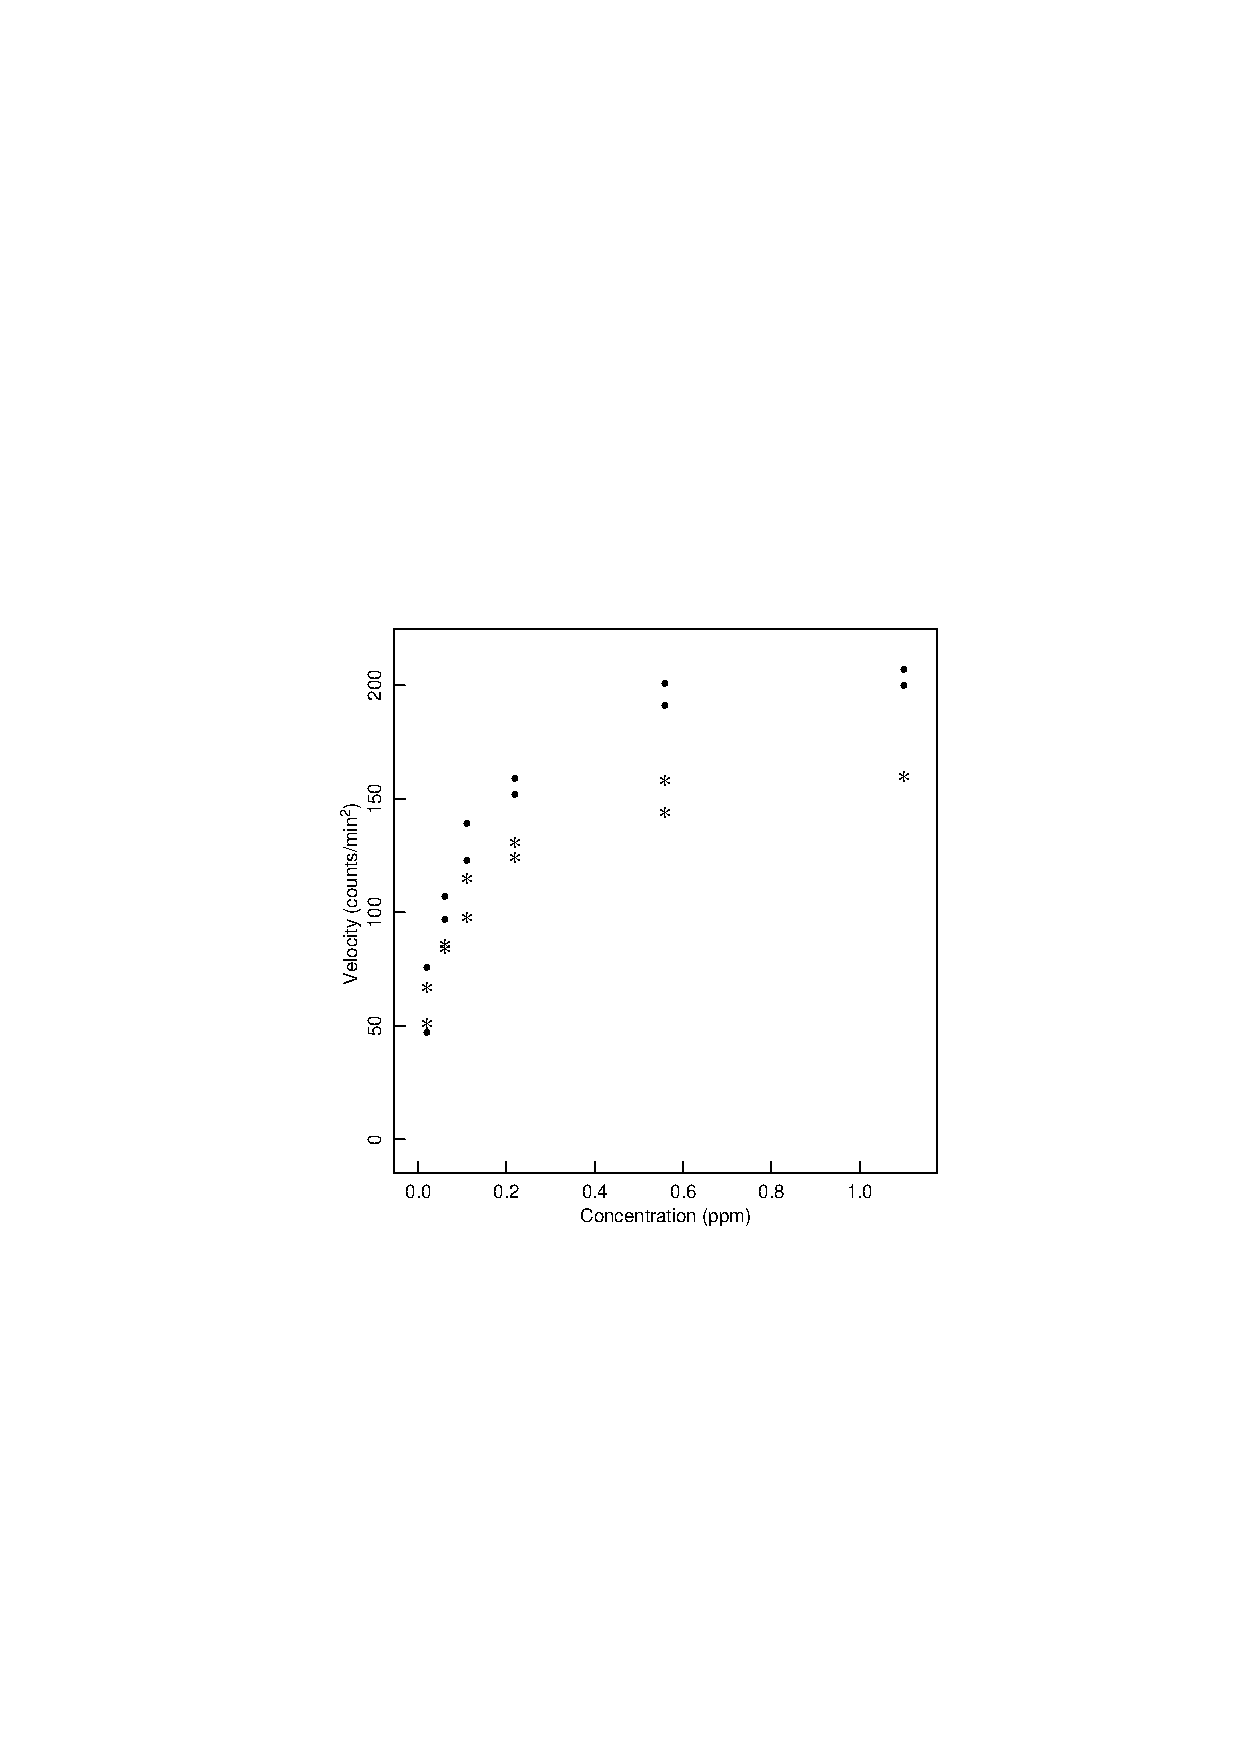
\includegraphics{3MIC2data}}%,height=3in}}
    \caption{Plot of enzyme velocity data versus substrate concentration.
      The data for the enzyme treated (not treated) with Puromycin are
      shown as ().}
    \label{fig:MIC2data}
  \end{figure}
  
  To determine if the $\theta_{2}$ parameter is unchanged,
  we use an extra sum of squares analysis, which requires fitting a full and a
  partial model.
  The full model corresponds to completely different sets of
  parameters for the treated data and the untreated data, while
  the partial model corresponds to different $\theta_{1}$
  parameters but the same $\theta_{2}$ parameter.
  To combine the full and partial models, we introduce
  the \emph{indicator variable}
  \begin{displaymath}
    x_2 = \left\{ 
      \begin{array}{ll}
        0 & \mbox{\rm untreated}\\
        1 & \mbox{\rm treated}
      \end{array}
    \right.
  \end{displaymath}
  
  and let $x_1$ be the substrate concentration.
  The combined model is then written
  \begin{displaymath}\label{eqn:combin}
    f(\bx,\btheta)=\frac{(\theta_1 + \phi_1 x_2 ) x_1}{(\theta_2+\phi_2 x_2)+x_1}
  \end{displaymath}
  where
  $\theta_{1}$ is the maximum velocity for the untreated enzyme,
  $\phi_{1}$ is the incremental maximum velocity due to the
  treatment,
  $\theta_{2}$ is the (possibly common) ``half-velocity''
  point, and $\phi_{2}$ is the change in the half-velocity due to the
  treatment.
  Since we expect $\phi_{1}$ to be nonzero, we are interested
  in testing whether $\phi_{2}$ could be zero.
  
  The model (\ref{eqn:combin}) was fitted and the results of this fit are
  shown in Table~\ref{tbl:treloar3}.
  \begin{table}
    \caption{
      Parameter summary for the 4-parameter Michaelis--Menten model fitted
      to the combined Puromycin data set.
    }\label{tbl:treloar3}
    \begin{center}
      \begin{tabular}{cccccccc} \hline
        & &\multicolumn{1}{c}{Approx.}&&\multicolumn{4}{c}{Correlation}\\
        \multicolumn{1}{c}{Parameter} &\multicolumn{1}{c}{Estimate}& \multicolumn{1}{c}{Std. Err.}&\multicolumn{1}{c}{$t$ Ratio} &\multicolumn{4}{c}{Matrix}\\ \hline
        $\theta_{1}$ &160.3 & 6.90 & 23.2 &1.00\\
        $\theta_{2}$ & 0.0477 & 0.00828 & 5.8 & 0.77 & 1.00\\
        $\phi_{1}$ & 52.4 & 9.55 & 5.5 &--\/0.72 & --\/0.56 & 1.00\\
        $\phi_{2}$ & 0.0164 & 0.0114 &1.4 &--\/0.56 & --\/0.72 & 0.77 & 1.00\\ \hline
      \end{tabular}
    \end{center}
  \end{table}
  It appears that $\phi_{2}$ could be zero, since it has a small
  $t$ ratio, and so we fit the
  partial model (\ref{eqn:combin}) with $\phi_2 = 0$.
  The results of this fit are given in
  Table~\ref{tbl:treloar4} and
  \begin{table}
    \caption{
      Parameter summary for the 3-parameter Michaelis--Menten model fitted
      to the combined Puromycin data set.
    }\label{tbl:treloar4}
    \begin{center}
      \begin{tabular}{ccccccc}\hline
        & & \multicolumn{1}{c}{Approx.}&&\multicolumn{3}{c}{Correlation}\\
        \multicolumn{1}{c}{Parameter} &\multicolumn{1}{c}{Estimate}& \multicolumn{1}{c}{Std. Err.} &\multicolumn{1}{c}{$t$ Ratio} & \multicolumn{3}{c}{Matrix}\\ \hline
        $\theta_{1}$&166.6&5.81&28.7&1.00\\
        $\theta_{2}$&0.058&0.00591&9.8&0.61&1.00\\
        $\phi_{1}$&42.0&6.27&6.7&--\/0.54&0.06&1.00\\ \hline
      \end{tabular}
    \end{center}
  \end{table}
  the extra sum of squares analysis is presented in
  Table~\ref{tbl:treloar}.
  \begin{table}
    \caption{
      Extra sum of squares analysis for the 3- and 4-parameter
      Michaelis--Menten model fitted to the combined Puromycin data set.
    }\label{tbl&treloar}
    \begin{center}
      \begin{tabular}{cccccc}\hline
        & \multicolumn{1}{c}{Sum of} & \multicolumn{1}{c}{Degrees of}
        &\multicolumn{1}{c}{Mean}\\ \multicolumn{1}{c}{Source} &
        \multicolumn{1}{c}{Squares} &\multicolumn{1}{c}{Freedom} &
        \multicolumn{1}{c}{Square} & \multicolumn{1}{c}{F Ratio}
        &\multicolumn{1}{c}{$p$ Value}\\
        \hline Extra&186&1&186.&1.7&0.21\\
        4-parameter&2055&19&108.2\\
        3-parameter&2241&20\\ \hline
      \end{tabular}
    \end{center}
  \end{table}
  
  In this well-designed experiment, which includes replications, it
  is also possible to analyze for lack of fit of the partial model as
  shown in Table~\ref{tbl:treloar5}.
  \begin{table}
    \caption{
      Lack of fit analysis for the 3-parameter Michaelis--Menten model
      fitted to the combined Puromycin data set.  }\label{tbl&treloar5}
    \begin{center}
      \begin{tabular}{cccccc}
        & \multicolumn{1}{c}{Sum of} & \multicolumn{1}{c}{Degrees
          of} & \multicolumn{1}{c}{Mean}\\ \multicolumn{1}{c}{Source} &
        \multicolumn{1}{c}{Squares} & \multicolumn{1}{c}{Freedom} &
        \multicolumn{1}{c}{Square} & \multicolumn{1}{c}{F Ratio} &
        \multicolumn{1}{c}{$p$ Value}\\ \hline
        Lack of fit &1144&9&127.3&1.3&0.35\\
        Replication&1097&11&99.7\\ \hline
        Residuals&2241&20\\ \hline
      \end{tabular}
    \end{center}
  \end{table}
  These summary calculations, together with plots of the residuals
  (not shown), suggest that a model which has a common
  half-velocity parameter and a higher asymptotic velocity for
  the treated enzyme is adequate.
\end{example}

In the above example, the $t$ ratios for the
incremental parameters permit reliable
inferences to be made concerning changes from one block to
another.
We recommend, however, that the extra sum of squares analysis
always be used,
since it is unaffected by parameter effects
nonlinearity (see Chapter 7) and is therefore more exact than the $t$ test
in the nonlinear case.
We only use the $t$ ratios to suggest which incremental
parameters might be zero and should be investigated
further:
the actual decision on whether to retain a parameter should be based on an
extra sum of squares analysis or a profile $t$ analysis (see Chapter 6).

In summary, incremental parameters provide a direct and simple
procedure for determining whether changes in parameters occur
between different blocks.
Clearly, incremental parameters can also be used
to advantage in linear least squares to
determine changes in parameters between blocks, since then the
$t$ tests are exact.
Even for linear least squares, however, we recommend fitting the
reduced model and using the extra sum of squares analysis to
make any final decisions concerning inclusion or deletion of
parameters, so as to avoid problems with multicollinearity and inflation
of variances.
Incremental parameters can also be used when there are more than
two blocks by introducing additional indicator variables or,
possibly, by rewriting the parameters as functions of other
variables as in Section 3.11.

\subsection{Non-nested Models}

When trying to decide which of several \emph{non-nested} models is
best, the first approach should be to the researcher.
That is, if there are scientific reasons for preferring one model
over the others, strong weight should be given to the
researcher's reasons because the primary aim of data analysis is
to explain or account for the behavior of the data, not simply to
get the best fit.

If the researcher cannot provide convincing reasons for choosing
one model over others, then statistical analyses can be used, the
most important of which is probably an analysis of the residuals.
Generally the model with the smallest residual mean square and
the most random-looking residuals should be chosen.
The residuals should be plotted versus the predicted values, the
control variables, time order, and any other (possibly lurking)
variables; see Section 3.7.

\section{Parameters as Functions of Other Variables}
\index{practical considerations!parameters as functions of other variables}
\index{parameter!as functions of other variables}

In many situations, the parameters in a mechanistic model will
depend on other variables.
For example, in chemical kinetic studies, we may have data from
several experiments in which the operating conditions have been
varied, and it may be thought that the rate constants should depend in
some systematic way on the operating conditions.
We would then like to fit a model which
incorporates the dependence of the \emph{kinetic parameters}
$\btheta$ on some \emph{process variables}, say $\bw$, and some
\emph{process parameters},
\index{parameter!process}
$\bphi = ( \phi_1 ,\ldots, \phi_L ) \trans$.
That is, $\btheta = \btheta ( \bw , \bphi )$.
The expectation function is then
$f ( \bx , \btheta ) = f ( \bx , \btheta ( \bw , \bphi ) )$.

To estimate the parameters in such an extended model, we could express
the function in terms of the regular variables $\bx$, the process
variables $\bw$, and the process parameters $\bphi$, determine the
derivatives with respect to $\bphi$, and then use a Gauss--Newton
algorithm to converge to $\hat{\bphi}$.
It is more efficient, however, to build on what we already have
and proceed as follows:
\begin{enumerate}
\item At each level of $\bw$, estimate the kinetic parameters
  $\btheta$ in the regular model.
\item Plot the parameter estimates $\hat \theta_{p}$ versus $\bw$
  to determine a plausible form for the relationship of $\hat
  \theta_{p}$ to $\bw$ and to obtain starting estimates for
  the process parameters $\bphi$.
\item  Use the chain rule for derivatives to determine the
  derivatives with respect to $\bphi$, exploiting the existing
  derivatives with respect to $\btheta$, as
  \begin{displaymath}
    \frac{\partial\eta_n}{\partial\phi_l}=\sum_{p=1}^P
    \frac{\partial\eta_n}{\partial\theta_p} 
    \frac{\partial\theta_p}{\partial\phi_l}
  \end{displaymath}
  for $l= 1 ,2 ,\ldots, L$, where $L$ is the total number of
  process parameters.
\end{enumerate}
An application of this method is described in Section 5.5.

\begin{example}\label{mic:pfunc}

  Suppose in the research on Puromycin (Example Puromycin \ref{mic:10})
  there were, say, four treatment levels of Puromycin instead of
  just two (treated and untreated).
  We could then proceed by incorporating three indicator variables to
  account for changes in the parameters due to different
  treatments.
  However, if the Puromycin treatments consist of different doses,
  it might be possible to write
  \begin{displaymath}
    f ( x , \btheta ) = \frac{\theta_1(w)x}{\theta_2(w)+x}
  \end{displaymath}
  where a possible form of $\theta_{1}$ and $\theta_{2}$ is
  \begin{eqnarray*}
    \theta_1&=&\phi_{10} + \phi_{11}  w\\
    \theta_2&=&\phi_{20} + \phi_{21}  w
  \end{eqnarray*}
  In this example, the (regular) variable is $x$, the substrate
  concentration, and the process variable is $w$, the Puromycin
  concentration.
  
  Now suppose that at Puromycin concentration $w_{1}$ we get
  estimates
  $\hat \theta_{11}$ and $\hat \theta_{21}$, at concentration
  $w_{2}$, we get estimates $\hat \theta_{12}$ and $\hat \theta_{22}$,
  and so on, and that a plot of $\hat \theta_{2}$ versus $w$ looks
  essentially flat, which suggests
  $\theta_2 =\mbox{\rm constant}$.
  Then we would choose $\phi_{20} = \hat \theta_{2}$.
  Suppose further that the plot of $\hat \theta_{1}$ versus $w$
  reveals a straight line relationship,
  $\theta_1 = \phi_{10} + \phi_{11} w$.
  We could then use linear regression of $\hat \theta_{1}$ on $w$
  to get starting estimates for $\phi_{10}$ and $\phi_{11}$.
  
  The model to be fitted to the combined data vector would be
  \begin{eqnarray*}
    f(x,w,\bphi)&=&\frac{\theta_1(w)x}{\theta_2(w)+x}\\
    &=&\frac{(\phi_{10}+\phi_{11}w)x}{\phi_{20}+x}
  \end{eqnarray*}
\end{example}

\section{Presenting the Results}
\index{practical considerations!presenting the results}
\index{report!writing}

As in all statistical analyses,
the results from a nonlinear regression analysis should be
presented clearly and succinctly.
This is usually done most effectively by considering the needs
and abilities of the prospective audience.
The report should always include a summary of the main findings
and conclusions.

The summary should include a
statement of the final model, the parameter estimates and their
standard errors, and an interpretation of the model and the
parameters in the context of the original problem.

In the main body of the report, it is useful to state the
original problem and possibly a derivation of the general form of
mechanistic model proposed.
Plots of the data should be given, and any preliminary analyses
should be discussed, particularly if they involved transformation
of the data or the expectation function.
A listing of the data should always be included (perhaps in an
appendix), but otherwise plots should be used for effective
communication.

The initial model should be presented with a brief
description of the steps taken to reduce or extend it, if
necessary referring to detailed analyses in appendices.
The final model, together with parameter estimates and their
approximate standard errors and correlation matrix should be
stated, along with a plot of the data, the fitted expectation
function, and an approximate confidence band for the
expectation function.
Pairwise plots of the parameter inference region,
and possibly profile $t$ plots,
as described in Chapter 6, should be given.
Of great importance is an interpretation of the expectation
function and the parameter values relative to the original
problem, and especially any new findings, such as the need for
additional variables in the model or the non-necessity of any
variables or parameters.

Finally, conclusions and recommendations should be made,
especially concerning possible future experiments or development
of the research.

For further tips on report writing, see \citeasnoun{ehre:1981},
%\glossary{ Ehrenberg, A.S.C.}
\citeasnoun{ehre:1982}, and \citeasnoun{watt:1981}.
%\glossary{ Watts, D.G.}
The preparation and presentation of graphical material is covered in
\citeasnoun{tuft:1983}, \citeasnoun{clev:1984},
\citeasnoun{clev:1985}, and \citeasnoun{cham:clev:klei:tuke:1983}.
%\glossary{ Tufte, E.R.}
%\glossary{ Cleveland, W.S.}
%\glossary{ Chambers, J.M.}
%\glossary{ Kleiner, B.}
%\glossary{ Tukey, P.W.}

\section{Nitrite Utilization:  A Case Study}

To illustrate the techniques presented in this chapter, we present an
analysis of data on the utilization of nitrite in bush beans as
a function of light intensity \cite{elli:peir:1986}.
%\glossary{ Elliott, J.R.}
%\glossary{ Peirson, D.R.}
Portions of primary leaves from three
16-day-old bean plants were subjected to eight levels of light
intensity ($\mu$E/m$^{2}$s), and the nitrite utilization
(nmol/ghr) was measured.
The experiment was repeated on a different day, resulting in the
data listed in Appendix~\ref{atbl:nitrite}.

The experimenters did not have a theoretical mechanism to explain
the behavior, but they thought that nitrite utilization should be
zero at zero light intensity, and should tend to an asymptote as
light intensity increased.
\subsection{Preliminary Analysis}
\index{preliminary analysis!nitrite example}

From a plot of the data
\begin{figure}
  \centerline{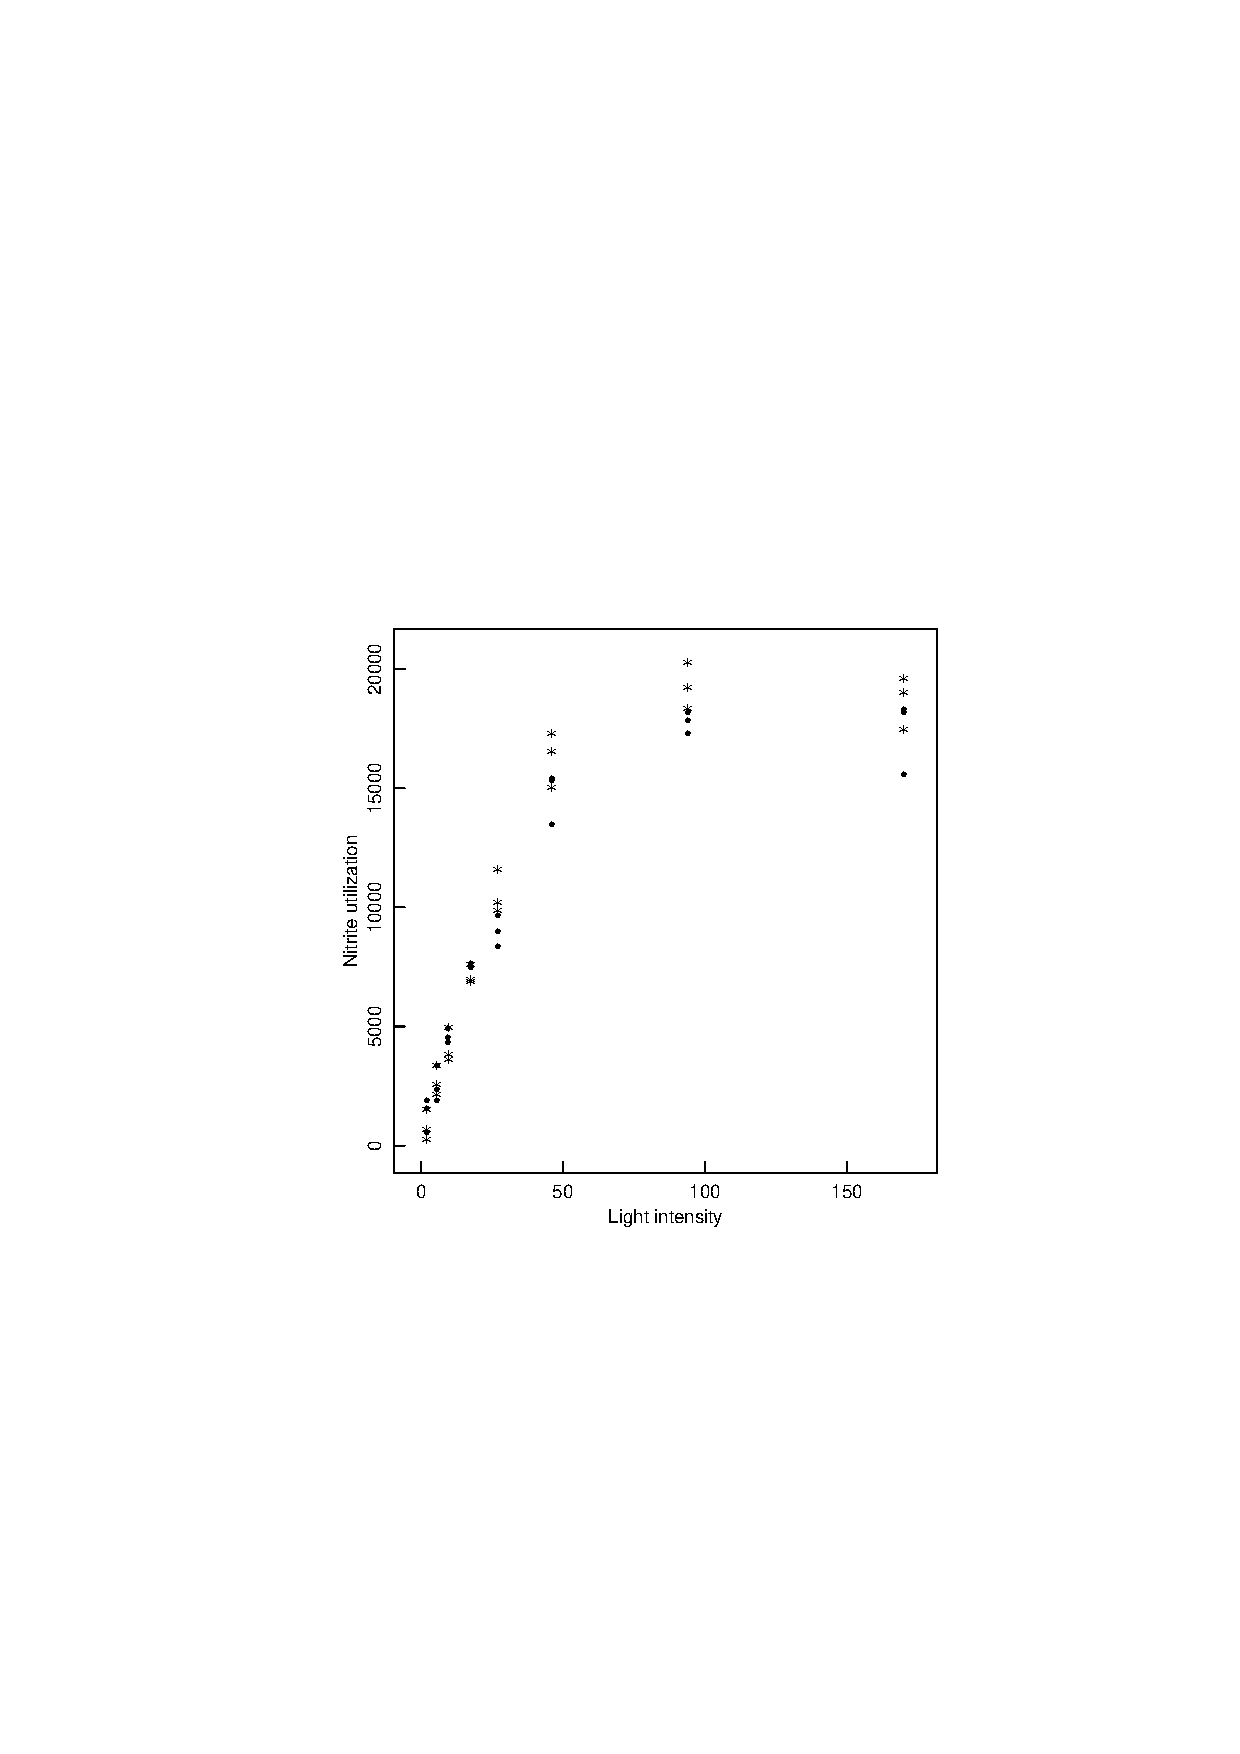
\includegraphics{3NITdata}}%,height=3in}}
  \caption{Plot of nitrite utilization by bean plants
    versus light intensity for day 1 (*) and day 2 ().}
  \label{fig:NITdata}
\end{figure}
(Figure~\ref{fig:NITdata}) it can be seen that there
was a difference in the nitrite utilization
between experiments on the two days,
particularly at higher light intensities.
There is also a tendency for the response to drop at high light
intensity.
Note too that, even though the response ranges from 200 to 20000
nmol/ghr, the variance is effectively constant;  there is no
need to transform to stabilize variance.
To verify the apparent stable variance, we performed a two way
analysis of variance using indicator variables for days and for
\index{analysis of variance!nitrite example}
\index{indicator variable!nitrite example}
light intensities, with the results shown in
Tables~\ref{tbl:3.2} and \ref{tbl:3.3}.
\begin{table}
  \caption{
  Two way analysis of variance for the nitrite utilization data.
  }\label{tbl:3.2}
  \begin{center}
    \begin{tabular}{cccccc}\hline
      &\multicolumn{1}{c}{Sum of} & \multicolumn{1}{c}{Degrees}
      &\multicolumn{1}{c}{Mean}\\ & \multicolumn{1}{c}{Squares} &
      \multicolumn{1}{c}{of} &\multicolumn{1}{c}{Square}\\
      \multicolumn{1}{c}{Source} & \multicolumn{1}{c}{$( 10^6 )$} &
      \multicolumn{1}{c}{Freedom} & \multicolumn{1}{c}{$( 10^6 )$} &
      \multicolumn{1}{c}{F Ratio} & \multicolumn{1}{c}{$p$ Value}\\ \hline
      Days&4.23&1&4.23&6.1&0.02\\
      Intensity&2040&7&291.5&420.&0.00\\
      Days$\times$intensity&10.07&7&1.44&2.1&0.08\\ \hline
      Replication&22.21&32&0.694\\ \hline
    \end{tabular}
  \end{center}
\end{table}
\begin{table}
  \caption{
  Replication averages and standard deviations for the nitrite
  utilization data.}\label{tbl:3.3}
  \begin{center}
    \begin{tabular}{ccccc}\hline
      &\multicolumn{2}{c}{Day 1} & \multicolumn{2}{c}{Day 2}\\ \hline
      && \multicolumn{1}{c}{Standard} && \multicolumn{1}{c}{Standard}\\
      \multicolumn{1}{c}{Intensity}
      &\multicolumn{1}{c}{Average}&\multicolumn{1}{c}{Deviation} &
      \multicolumn{1}{c}{Average} & \multicolumn{1}{c}{Deviation}\\ \hline
      2.2&826&652&1327&694\\
      5.5&2702&623&2541&758\\
      9.6&4136&719&4619&296\\
      17.5&7175&401&7554&86\\
      27.0&10567&908&9019&650\\
      46.0&16302&1154&14753&1082\\
      94.0&19296&963&17786&430\\
      170.0&18719&1117&17374&1408\\ \hline
    \end{tabular}
  \end{center}
\end{table}
For our purposes the most useful information from the two way analysis
of variance is the replication sum of squares and mean square,
which can be used for testing lack of fit.
We note, however, that the lack of a significant
day$\times$intensity interaction suggests that some of the model parameters
may be equal for the two days, although the
significant day effect tends to corroborate the observed
difference between the heights of the maxima on the two days.
A plot of the replication
\begin{figure}
  \centerline{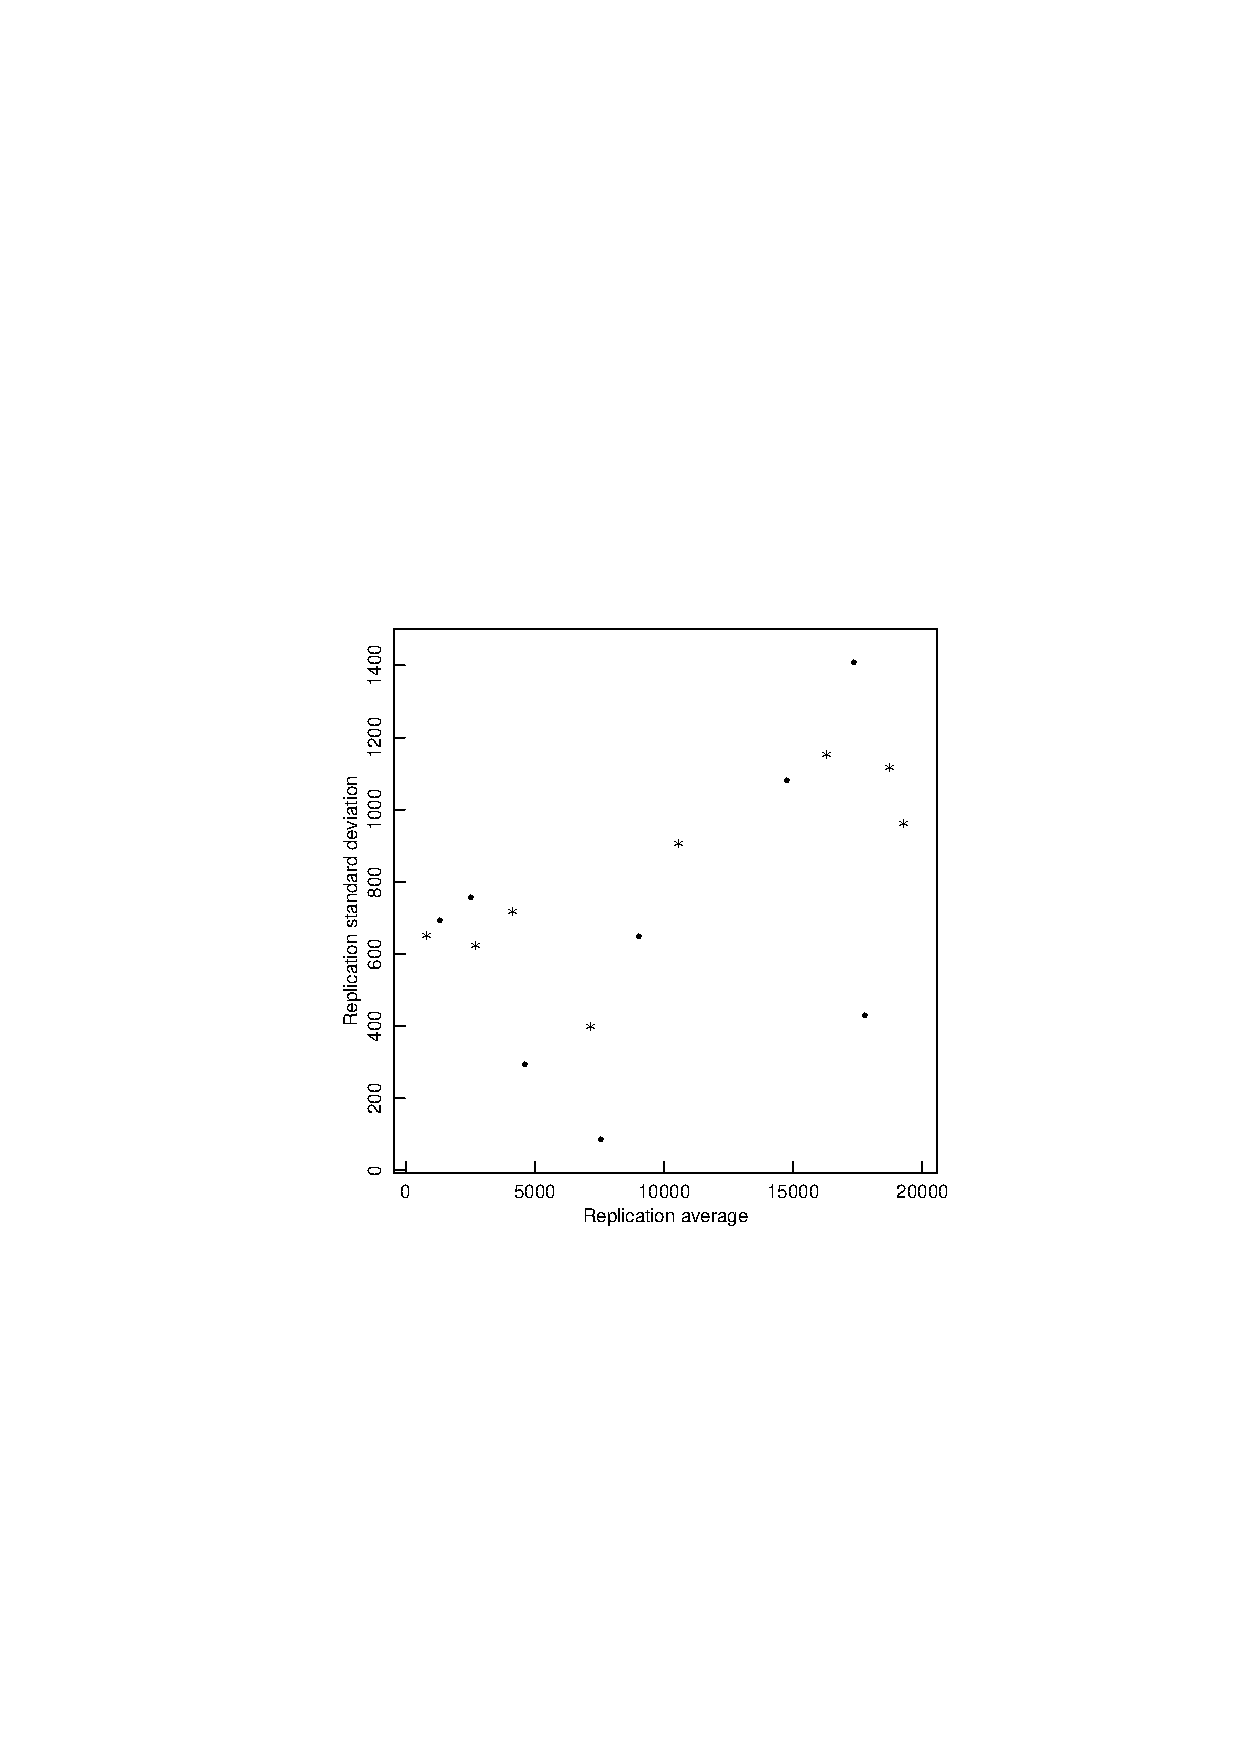
\includegraphics{3NITrep}}%,height=2.75in}}
  \caption{Replication standard deviations plotted versus replication
    averages for the nitrite utilization data.  Day 1 data are shown
    as $*$ and day 2 data as .}
  \label{fig:NITrep}
\end{figure}
standard deviations versus the replication averages, shown in
Figure~\ref{fig:NITrep}, verified our earlier assessment that the
variance is stable since there is no systematic relation,
and so we proceed to model fitting.

Note that the analysis of variance is used here only as a screening
tool.
It is not intended as a final analysis of these data, since the
underlying additive linear model assumed in an analysis of variance is
not appropriate.

\subsection{Model Selection}
\index{model!selection, nitrite example}

Because the researchers did not have a model in mind, it was
necessary to select one on the basis of the behavior of the data.
The Michaelis--Menten model
\begin{displaymath}
  f(x,\btheta)=\frac{\theta_1x}{\theta_2+x}
\end{displaymath}
and the simple exponential rise model
\begin{displaymath}
f (x , \btheta ) = \theta_1 ( 1 - e^{ - \theta_2 x } )
\end{displaymath}
were selected because they met the researcher's beliefs
that nitrite utilization was zero at zero light intensity and tended to
an asymptote as the light intensity increased.
To simplify the description, we give details for the
Michaelis--Menten model analysis, and only present summaries for
the exponential rise model.

Since there are 24 observations for each day from this
well-designed experiment, it would be reasonable to fit a
separate model for each day.
We would like to think, however, that the same
parameter values, or at least some of the same
parameter values, would be valid for both days, and so
we proceed to fit a model for day 1 with incremental
parameters for day 2.
\index{incremental parameter!nitrite example}
That is, we write
\begin{displaymath}
f(x,\btheta)=\frac{(\theta_1+\phi_1x_2)x_1}{(\theta_2+\phi_2 x_2)+x_1}
\end{displaymath}
where $x_{1}$ is the light intensity and $x_{2}$ is an
indicator variable
\begin{displaymath}
x_2 = \left\{
  \begin{array}{l l}
    0&\mbox{\rm day 1}\\
    1&\mbox{\rm day 2}
  \end{array}\right.
\end{displaymath}
as described in Section 3.10.

\subsection{Starting Values}

Since the maximum value on day 1 is about 20,000, and on day 2 is
about 18,000, we choose $\theta_1^0=25000$ and
$\phi_1^0=-3000$.
The response reaches about 12500 at a light intensity of about 34
for day 1 and 35 for day 2, which gives $\theta_2^0=34$ and
$phi_2^0=1$.

\subsection{Assessing the Fit}
\index{assessing fit!nitrite example}

Convergence was achieved at the values shown in
Table~\ref{tbl:3.4}.
\begin{table}
  \caption{
  Parameter summary for the 4-parameter Michaelis--Menten model
  fitted to the nitrite utilization data.
  }\label{tbl:3.4}
  \begin{center}
    \begin{tabular}{cccccccc}\hline
      &&\multicolumn{1}{c}{Standard}&&\multicolumn{4}{c}{Correlation}\\
      \multicolumn{1}{c}{Parameter}&\multicolumn{1}{c}{Estimate}&
      \multicolumn{1}{c}{Error}&\multicolumn{1}{c}{$t$ Ratio} &
      \multicolumn{4}{c}{Matrix}\\ \hline
      $\theta_{1}$&24743&1241&19.9&1.00\\
      $\theta_{2}$&35.27&4.66&7.6&0.88&1.00\\
      $\phi_{1}$&--2329&1720&--1.4&--\/0.72&--\/0.64&1.00\\
      $\phi_{2}$&--2.174&6.63&--\/0.3&--\/0.62&--\/0.70&0.88&1.00\\ \hline
    \end{tabular}
  \end{center}
\end{table}
It appears from the $t$ ratios that both the
incremental parameters could be estimates of zero, and so a
common model could be fitted.
However, if we do a lack of fit analysis on this model as in
\index{lack of fit!analysis, nitrite example}
Table~\ref{tbl:mic4lof},
we see that this four-parameter model is not adequate.
\begin{table}
  \caption{
  Lack of fit analysis for the 4-parameter Michaelis--Menten model
  fitted to the nitrite utilization data.}\label{tbl:mic4lof}
  \begin{center}
    \begin{tabular}{lccccc}\hline
      &\multicolumn{1}{c}{Sum of} &\multicolumn{1}{c}{Degrees}
      &\multicolumn{1}{c}{Mean}\\ & 
      \multicolumn{1}{c}{Squares}& \multicolumn{1}{c}{of}
      &\multicolumn{1}{c}{Square}\\ 
      Source&\multicolumn{1}{c}{$(10^6 )$}&\multicolumn{1}{c}{Freedom}
      &\multicolumn{1}{c}{$(10^6 )$} &\multicolumn{1}{c}{F Ratio}&
      \multicolumn{1}{c}{$p$ Value}\\ \hline
      Lack of fit&64.30&12&5.36&7.72&0.00\\
      Replications&22.21&32&0.694\\ \hline
      Residuals&86.51&44\\ \hline
    \end{tabular}
  \end{center}
\end{table}
(The same conclusion was reached for the exponential rise model,
in this case with a lack of fit ratio of 3.2,
corresponding to a $p$ value of 0.00.)

A plot of the residuals versus light intensity,
as in
\begin{figure}
  \centerline{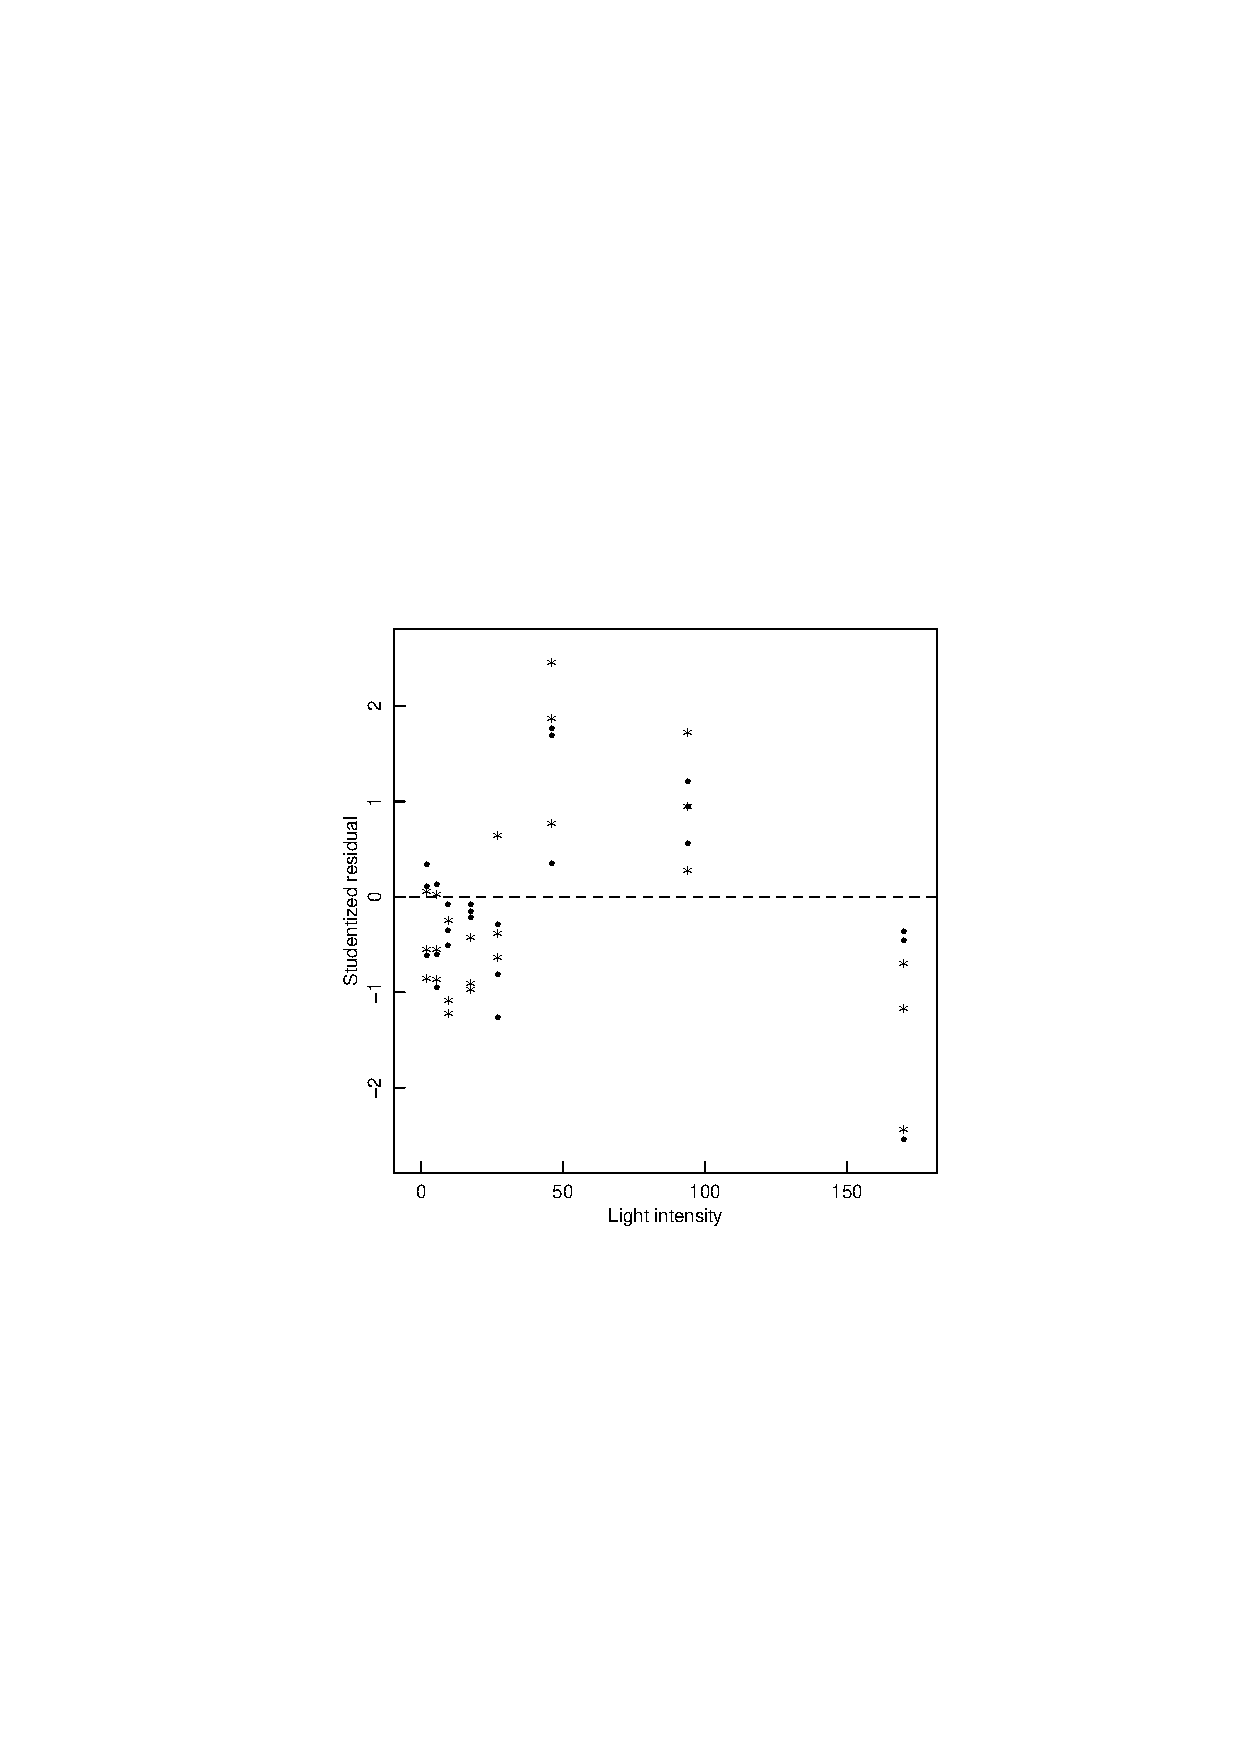
\includegraphics{3NITres1}}%,height=3in}}
  \caption{Studentized residuals from the 4-parameter
    Michaelis--Menten model plotted versus light intensity.  Day 1
    data are shown as $*$ and day 2 data as .}
\label{fig:NITres1}
\end{figure}
Figure~\ref{fig:NITres1}, reveals nonrandom
behavior, with negative residuals at small and large intensities
and positive ones in the middle.
The model must therefore be modified to allow the nitrite
utilization to drop with increasing light intensity, rather than
leveling off as suggested by the researchers.

\subsection{Modifying the Model}

To alter the Michaelis--Menten expectation function to rise to a
peak and then fall, we added a quadratic term to the denominator to
produce the quadratic Michaelis--Menten model,
\begin{displaymath}
  f(x,\btheta)=\frac{\theta_1x}{\theta_2+x+\theta_3x^2}
\end{displaymath}
which, with incremental parameters and an indicator variable
for the different days, becomes
\begin{displaymath}
  f(\bx,\btheta)=\frac{(\theta_1+\phi_1 x_2)x_1}{(\theta_2+\phi_2x_2)+x_1
    +(\theta_3+\phi_3x_2)x_1^2}
\end{displaymath}
(For the exponential rise model, we replaced the unit term by an
exponential to produce the exponential difference model,
\begin{displaymath}
f = \theta_1 ( e^{ - \theta_3 x } -
e^{ - \theta_2 x } )
\end{displaymath}
This model, augmented with increment parameters and an
indicator variable, was also used to fit the data.)

Starting values for the parameters were obtained by taking
reciprocals of the function and the data and using linear least
squares for the quadratic Michaelis--Menten model.
Taking reciprocals worked for the day 2 data, giving
$\btheta=(107411,234,0.024)\trans$, but gave some
negative values for the day 1 data.
We therefore used the day 2 starting values with slight
perturbations to get starting values for the 6-parameter model of
$\btheta^0=( 110000 ,234 ,0.024 ) \trans$ and
$\bphi^0=( -10000 ,23 ,0.002 ) \trans$.
(For the exponential difference model, we guessed that the two
rate constants might be in the ratio 1:5 and used the estimate
for $\theta_{2}$ to give $\theta_3 =0.006$.
We then estimated $\theta_{1}$ by evaluating
\begin{displaymath}
  \theta_1=\frac{y}{e^{{-0.006x}}-e^{{-0.030x}}}
\end{displaymath}
for several $x$ values.  This gave $\theta_1^{0}=37000$
for the day 1 data and $35000$ for the day 2 data, from which we
got $\phi_1^0 = -2000$.)

\subsection{Assessing the Fit}
\index{assessing fit!nitrite example}

Quick convergence was achieved
to the parameter estimates given in
Table~\ref{tbl:3.5} for the quadratic Michaelis--Menten model.
\begin{table}
  \caption{
  Parameter summary for the 6-parameter quadratic Michaelis--Menten model
  fitted to the nitrite utilization data.}\label{tbl:3.5}
  \begin{center}
    \begin{tabular}{ccccccccc}\hline
      &&\multicolumn{1}{c}{Standard}&&\multicolumn{5}{c}{Correlation}\\
      \multicolumn{1}{c}{Parameter}&\multicolumn{1}{c}{Estimate}&
      \multicolumn{1}{c}{Error}& \multicolumn{1}{c}{$t$ Ratio} &
      \multicolumn{5}{c}{Matrix}\\ \hline
      $\theta_{1}$&89846&37583&2.4&1.00\\
      $\theta_{2}$&186.7&90.1&2.1&1.00&1.00\\
      $\theta_{3}$&0.01626&0.00922&1.8&1.00&0.99&1.00\\
      $\phi_{1}$&--38956&40020&--1.0&--\/0.94&--\/0.94&--\/0.94&1.00\\
      $\phi_{2}$&--83.23&96.8&--\/0.9&--\/0.93&--\/0.93&--\/0.92&1.00&1.00\\
      $\phi_{3}$&--\/0.00846&0.0993&--\/0.9&--\/0.93&--\/0.92&--\/0.93&1.00&0.99\\ \hline
    \end{tabular}
  \end{center}
\end{table}
All the incremental parameters have nonsignificant approximate
$t$ ratios, which suggests that the parameters could be zero, and
so a simpler model may be adequate.
The extremely high parameter approximate correlations also lead one to
suspect that the model may be overparametrized.
\index{overparametrization!nitrite example}
The residual sum of squares ($32.02 \times 10^{6}$ on 42 df)
is only about a third of that for the previous model.
(Similar conclusions were reached for the 6-parameter exponential
difference model.)

The residuals for this model, plotted versus light intensity in
\begin{figure}
  \centerline{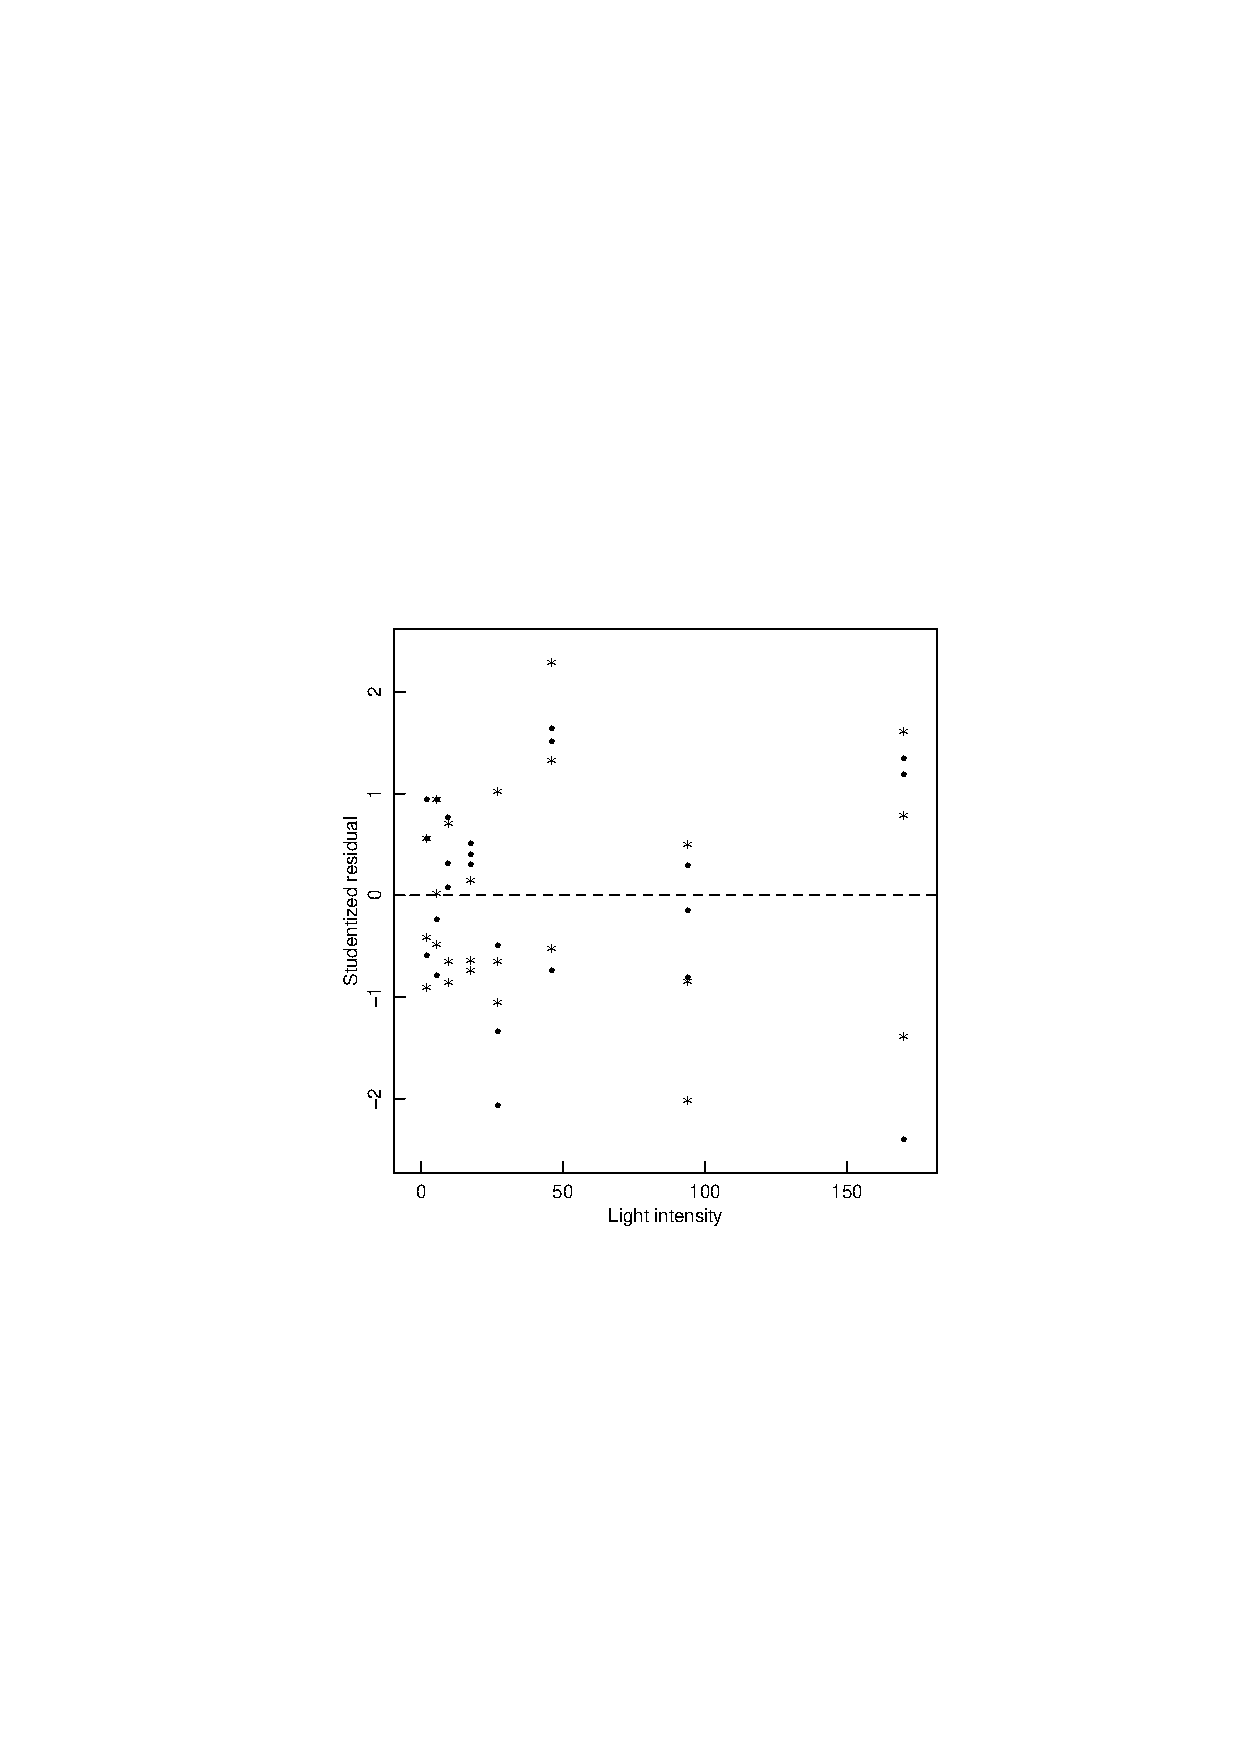
\includegraphics{3NITres2}}%,height=3in}}
  \caption{Studentized residuals from the 6-parameter quadratic
    Michaelis--Menten model plotted versus light intensity.  Day 1
    data are shown as * and day 2 data as $\cdot$.}
  \label{fig:NITres2}
\end{figure}
Figure~\ref{fig:NITres2}, are clearly well behaved and give no
evidence of inadequacy of the model.

\subsection{Reducing the Model}

To determine what simplifications could be made in the quadratic
Michaelis--Menten model,
we set $\phi_{2}$ and $\phi_{3}$ to zero,
still retaining $\phi_{1}$
to account for a difference between days.
For starting values, we simply used the relevant converged values
from the 6-parameter model.

\subsection{Assessing the Fit}
\index{assessing fit!nitrite example}

The results for the 4-parameter quadratic model are given in
Table~\ref{tbl:3.6}.
\begin{table}
  \caption{
  Parameter summary for the 4-parameter quadratic Michaelis--Menten model
  fitted to the nitrite utilization data.}\label{tbl:3.6}
  \begin{center}
    \begin{tabular}{cccccccc}\hline
      &&\multicolumn{1}{c}{Standard} &&\multicolumn{4}{c}{Correlation}\\
      Parameter & \multicolumn{1}{c}{Estimate}&
      \multicolumn{1}{c}{Error} &\multicolumn{1}{c}{$t$ Ratio} &
      \multicolumn{4}{c}{Matrix}\\ \hline 
      $\theta_{1}$&70096&16443&4.3&1.00\\
      $\theta_{2}$&139.4&39.3&3.6&1.00&1.00\\
      $\theta_{3}$&0.01144&0.00404&2.8&0.99&0.99&1.00\\
      $\phi_{1}$&--5381&1915&--2.8&--\/0.69&--\/0.66&--\/0.66&1.00\\ \hline
    \end{tabular}
  \end{center}
\end{table}
The extra sum of squares analysis for the 4-parameter
\index{extra sum of squares!nitrite example}
versus the 6-parameter quadratic model, shown in
Table~\ref{tbl:3.7},
\begin{table}
  \caption{
  Extra sum of squares analysis for the 6-parameter
  versus the 4-parameter quadratic Michaelis--Menten model
  fitted to the nitrite utilization data.
  }\label{tbl:3.7}
  \begin{center}
    \begin{tabular}{cccccc}\hline
      &\multicolumn{1}{c}{Sum of}&\multicolumn{1}{c}{Degrees}&
      \multicolumn{1}{c}{Mean}\\
      &\multicolumn{1}{c}{Squares} &\multicolumn{1}{c}{of}
      &\multicolumn{1}{c}{Square}\\ 
      \multicolumn{1}{c}{Source}&\multicolumn{1}{c}{$( 10^6 )$}
      &\multicolumn{1}{c}{Freedom}&\multicolumn{1}{c}{$( 10^6 )$}
      &\multicolumn{1}{c}{F Ratio} &\multicolumn{1}{c}{$p$ Value}\\ \hline
      Extra&0.82&2&0.41&0.54&0.59\\
      6-parameter&32.02&42&0.762\\ \hline
      4-parameter&32.84&44&0.746\\ \hline
    \end{tabular}
  \end{center}
\end{table}
does not show a significant degradation of the fit with
elimination of $\phi_{2}$ and $\phi_{3}$.
The residuals, when plotted versus light intensity as in
\begin{figure}
  \centerline{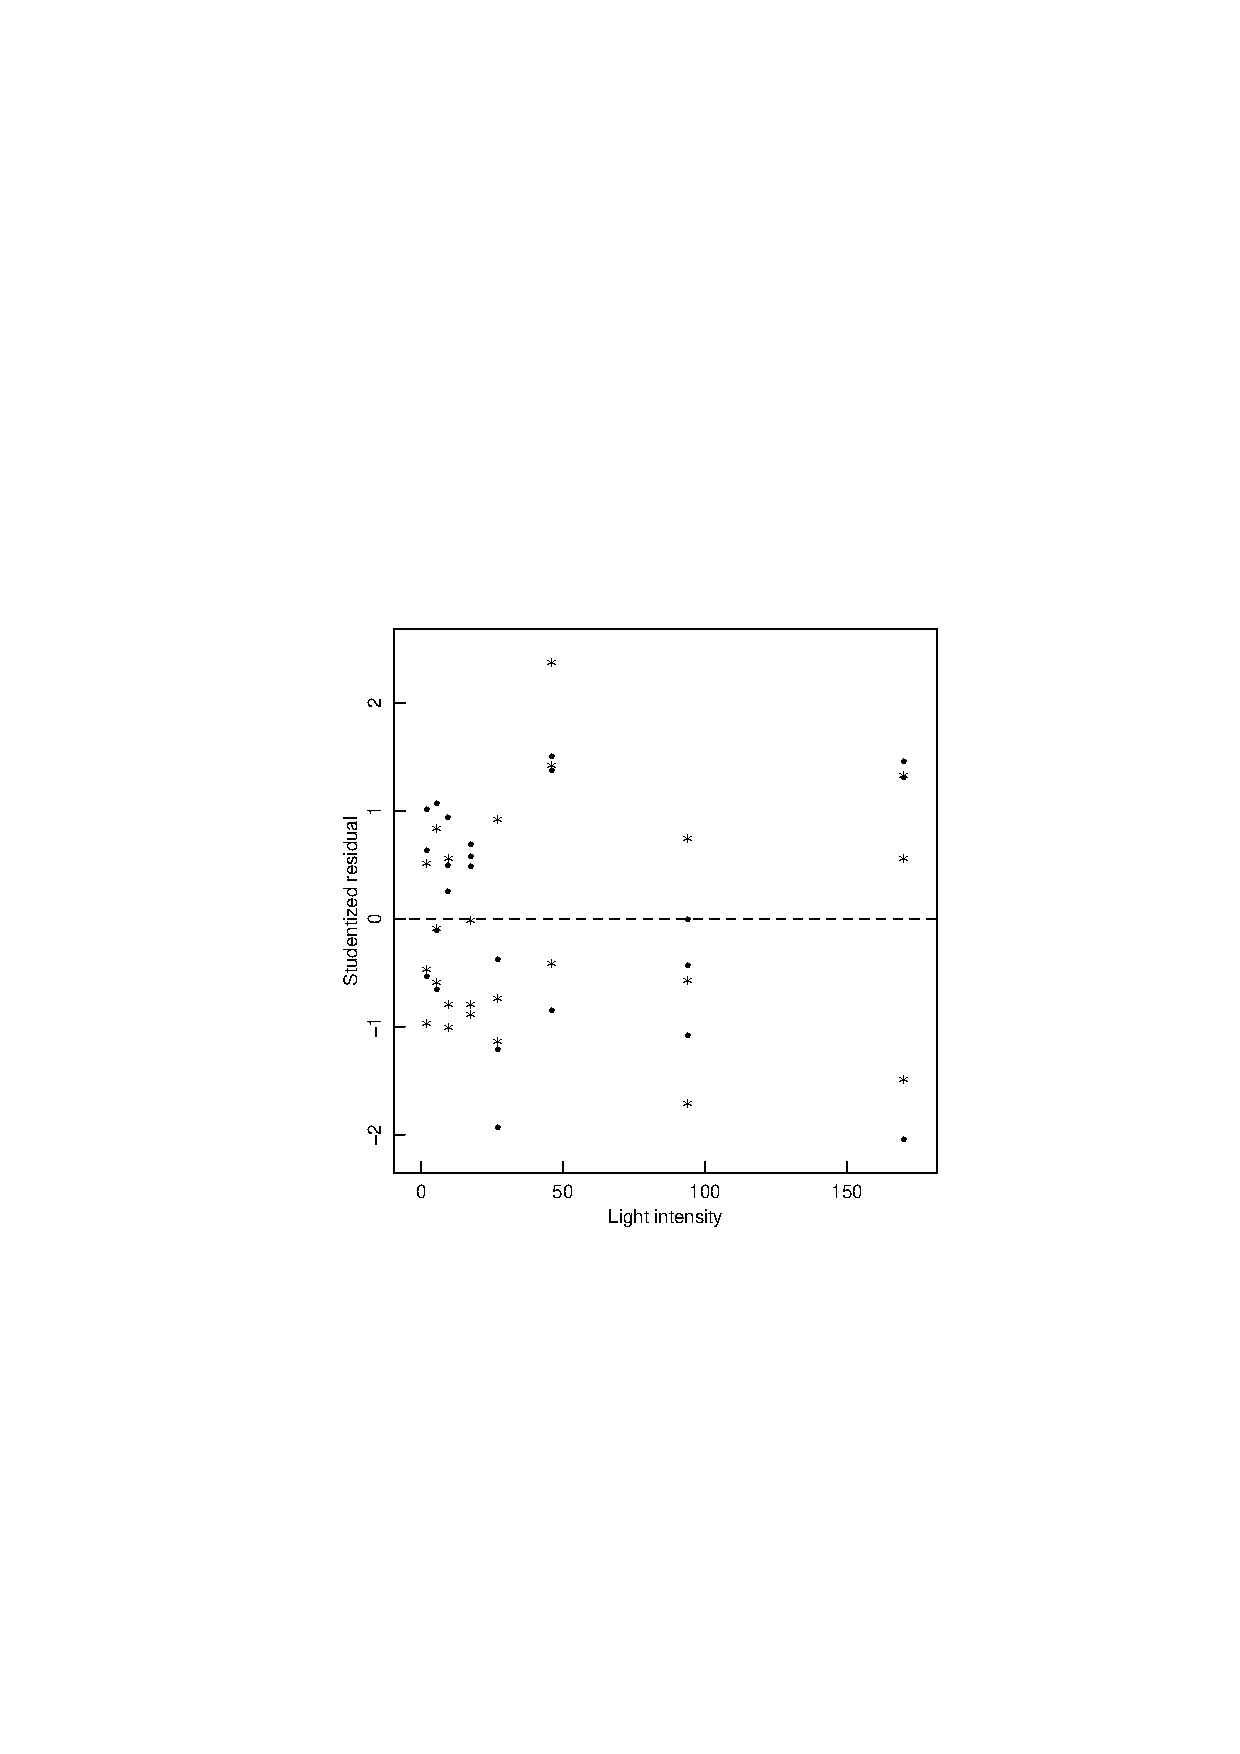
\includegraphics{3NITres3}}%,height=3in}}
  \caption{Studentized residuals from the 4-parameter quadratic
    Michaelis--Menten model plotted versus light intensity.  Day 1
    data are shown as * and day 2 data as $\cdot$.}
  \label{fig:NITres3}
\end{figure}
Figure~\ref{fig:NITres3}, attest to the adequacy of the model.
Furthermore, a lack of fit analysis, shown in
Table~\ref{tbl:qmic4lof}, suggests that the model is adequate.
\begin{table}
  \caption{Lack of fit analysis for the 4-parameter quadratic
    Michaelis--Menten model fitted to the nitrite utilization data.}
  \label{tbl:qmic4lof}
  \begin{center}
    \begin{tabular}{lccccc}\hline
      &\multicolumn{1}{c}{Sum of}&\multicolumn{1}{c}{Degrees}
      &\multicolumn{1}{c}{Mean}\\
      &\multicolumn{1}{c}{Squares} &\multicolumn{1}{c}{of} &
      \multicolumn{1}{c}{Square}\\
      \multicolumn{1}{c}{Source} & \multicolumn{1}{c}{$( 10^6 )$}
      &\multicolumn{1}{c}{Freedom} & \multicolumn{1}{c}{$( 10^6 )$} &
      \multicolumn{1}{c}{F Ratio} & \multicolumn{1}{c}{$p$ Value}\\ \hline
      Lack of fit&10.63&12&0.886&1.28&0.28\\
      Replications&22.21&32&0.694\\ \hline
      Residuals&32.84&44&0.746\\ \hline
    \end{tabular}
  \end{center}
\end{table}

Note that the parameter $\phi_{1}$ is now apparently
significantly different from 0, with an approximate
$t$ ratio of $-2.8$, confirming our earlier
suspicion that there was a difference between days.
This parameter was not significantly different from 0 in the
6-parameter model, which is further evidence for the 6-parameter
model being overparametrized and hence the parameter
approximate standard errors being artificially inflated, causing
nonsignificant $t$ ratios.

The parameter approximate correlation matrix for the quadratic
Michaelis--Menten 4-parameter model shown in
Table~\ref{tbl:3.6}
reveals that several of the correlations are very large.
This is not unusual in nonlinear regression, and is induced by a
combination of the form of the expectation function and the
design used.
For example, for a Michaelis--Menten model, no matter how good the
design is, it is impossible to obtain zero correlation between
the parameters because it is impossible to force the derivatives
to be orthogonal.
To see this, we note that the first column of
the derivative matrix, $\bv_{1}$, has elements
$x /( \theta_2 + x)$, and the second column,
$\bv_{2}$, has elements
${- \theta_1 x} / ( \theta_2 + x )^{2}$.
All the elements in $\bv_{1}$ are positive and all the
elements in $\bv_{2}$ are negative, and so the two vectors
$\bv_{1}$ and
$ - \bv_{2}$ will always tend to point in the same
direction in the response space.
Consequently, they will tend to be collinear.

As a final check on the model, the 3-parameter Michaelis--Menten
model
\begin{displaymath}
  f=\frac{(\theta_1+\phi_1x_2)x_1}{\theta_2+x_1}
\end{displaymath}
could be fitted and compared with the
4-parameter quadratic Michaelis--Menten model using an extra sum of
squares analysis to further substantiate the necessity for the parameter
$\theta_{3}$.
This was not done because the residuals for the original 3-parameter
Michaelis--Menten model were so badly behaved.

(Similar results and conclusions were reached for the exponential
difference model:  that is, a 4-parameter model with common
exponential parameters and scale factor, plus an incremental
parameter for day 2, was found to give an adequate fit.
Summary information on the fit is given in
Table~\ref{tbl:3.9},
\begin{table}
  \caption{Parameter summary for the 4-parameter exponential
    difference model fitted to the nitrite utilization data.}
  \label{tbl:3.9}
  \begin{center}
    \begin{tabular}{cccccccc} \hline
      &&\multicolumn{1}{c}{Standard} &&
      \multicolumn{4}{c}{Correlation}\\
      \multicolumn{1}{c}{Parameter} & \multicolumn{1}{c}{Estimate} &
      \multicolumn{1}{c}{Error} & \multicolumn{1}{c}{$t$ Ratio} &
      \multicolumn{4}{c}{Matrix}\\ \hline
      $\theta_{1}$&35115&8940&3.9&1.00\\
      $\theta_{2}$&0.01845&0.00317&5.8&--\/0.99&1.00\\
      $\theta_{3}$&0.00325&0.00120&2.7&0.99&--\/0.97&1.00\\
      $\phi_{1}$&$-2686$&1006&--2.7&--\/0.71&0.67&--\/0.68&1.00\\ \hline
    \end{tabular}
  \end{center}
\end{table}
and comparison with
the 6-parameter model in Table~\ref{tbl:3.10}.
\begin{table}
  \caption{
  Extra sum of squares analysis for the 6-parameter
  versus the 4-parameter exponential difference model
  fitted to the nitrite utilization data.
  }\label{tbl:3.10}
  \begin{center}
    \begin{tabular}{lccccc} \hline
      & \multicolumn{1}{c}{Sum of} & \multicolumn{1}{c}{Degrees} &
      \multicolumn{1}{c}{Mean}\\
      & \multicolumn{1}{c}{Squares} & \multicolumn{1}{c}{of} &
      \multicolumn{1}{c}{Square}\\
      \multicolumn{1}{c}{Source} & \multicolumn{1}{c}{$( 10^6 )$} &
      \multicolumn{1}{c}{Freedom} & \multicolumn{1}{c}{$( 10^6 )$} &
      \multicolumn{1}{c}{F Ratio} & \multicolumn{1}{c}{$p$ Value}\\ \hline
      Extra&0.37&2&0.19&0.23&0.80\\
      6-parameter&33.97&42&0.809\\ \hline
      4-parameter&34.34&44&0.780\\ \hline
    \end{tabular}
  \end{center}
\end{table}

The lack of fit analysis is given in Table~\ref{tbl:3.11}.
\begin{table}
  \caption{
  Lack of fit analysis for the 4-parameter exponential difference
  model fitted to the nitrite utilization data.}\label{tbl:3.11}
  \begin{center}
    \begin{tabular}{lccccc}\hline
      & \multicolumn{1}{c}{Sum of} & \multicolumn{1}{c}{Degrees} &
      \multicolumn{1}{c}{Mean}\\
      & \multicolumn{1}{c}{Squares} & \multicolumn{1}{c}{of} &
      \multicolumn{1}{c}{Square}\\
      \multicolumn{1}{c}{Source} & \multicolumn{1}{c}{$( 10^6 )$} &
      \multicolumn{1}{c}{Freedom} & \multicolumn{1}{c}{$( 10^6 )$} &
      \multicolumn{1}{c}{F Ratio} & \multicolumn{1}{c}{$p$ Value}\\ \hline
      Lack of fit&12.13&12&1.011&1.46&0.19\\
      Replications&22.21&32&0.694\\ \hline
      Residuals&34.34&44&0.780\\ \hline
    \end{tabular}
  \end{center}
\end{table}
In this case, the lack of fit ratio was 1.46, still not
significant, but slightly larger than for the quadratic
Michaelis--Menten model.)

\subsection{Comparing the Models}

To compare the nested models we have used incremental parameters
and the extra sum of squares principal, but they can not be used
to compare the quadratic Michaelis--Menten and the exponential
difference models.
Our first approach was to the researchers, asking them whether
one model was preferred on scientific grounds.
In this case, the researchers had no
preference, and so we simply presented them
with the results for both models.
Because the lack of fit ratio and the residual mean squares were
smaller, we had a slight preference for the Michaelis--Menten
model.
In Figure~\ref{fig:NITconfband}
\begin{figure}
  \centerline{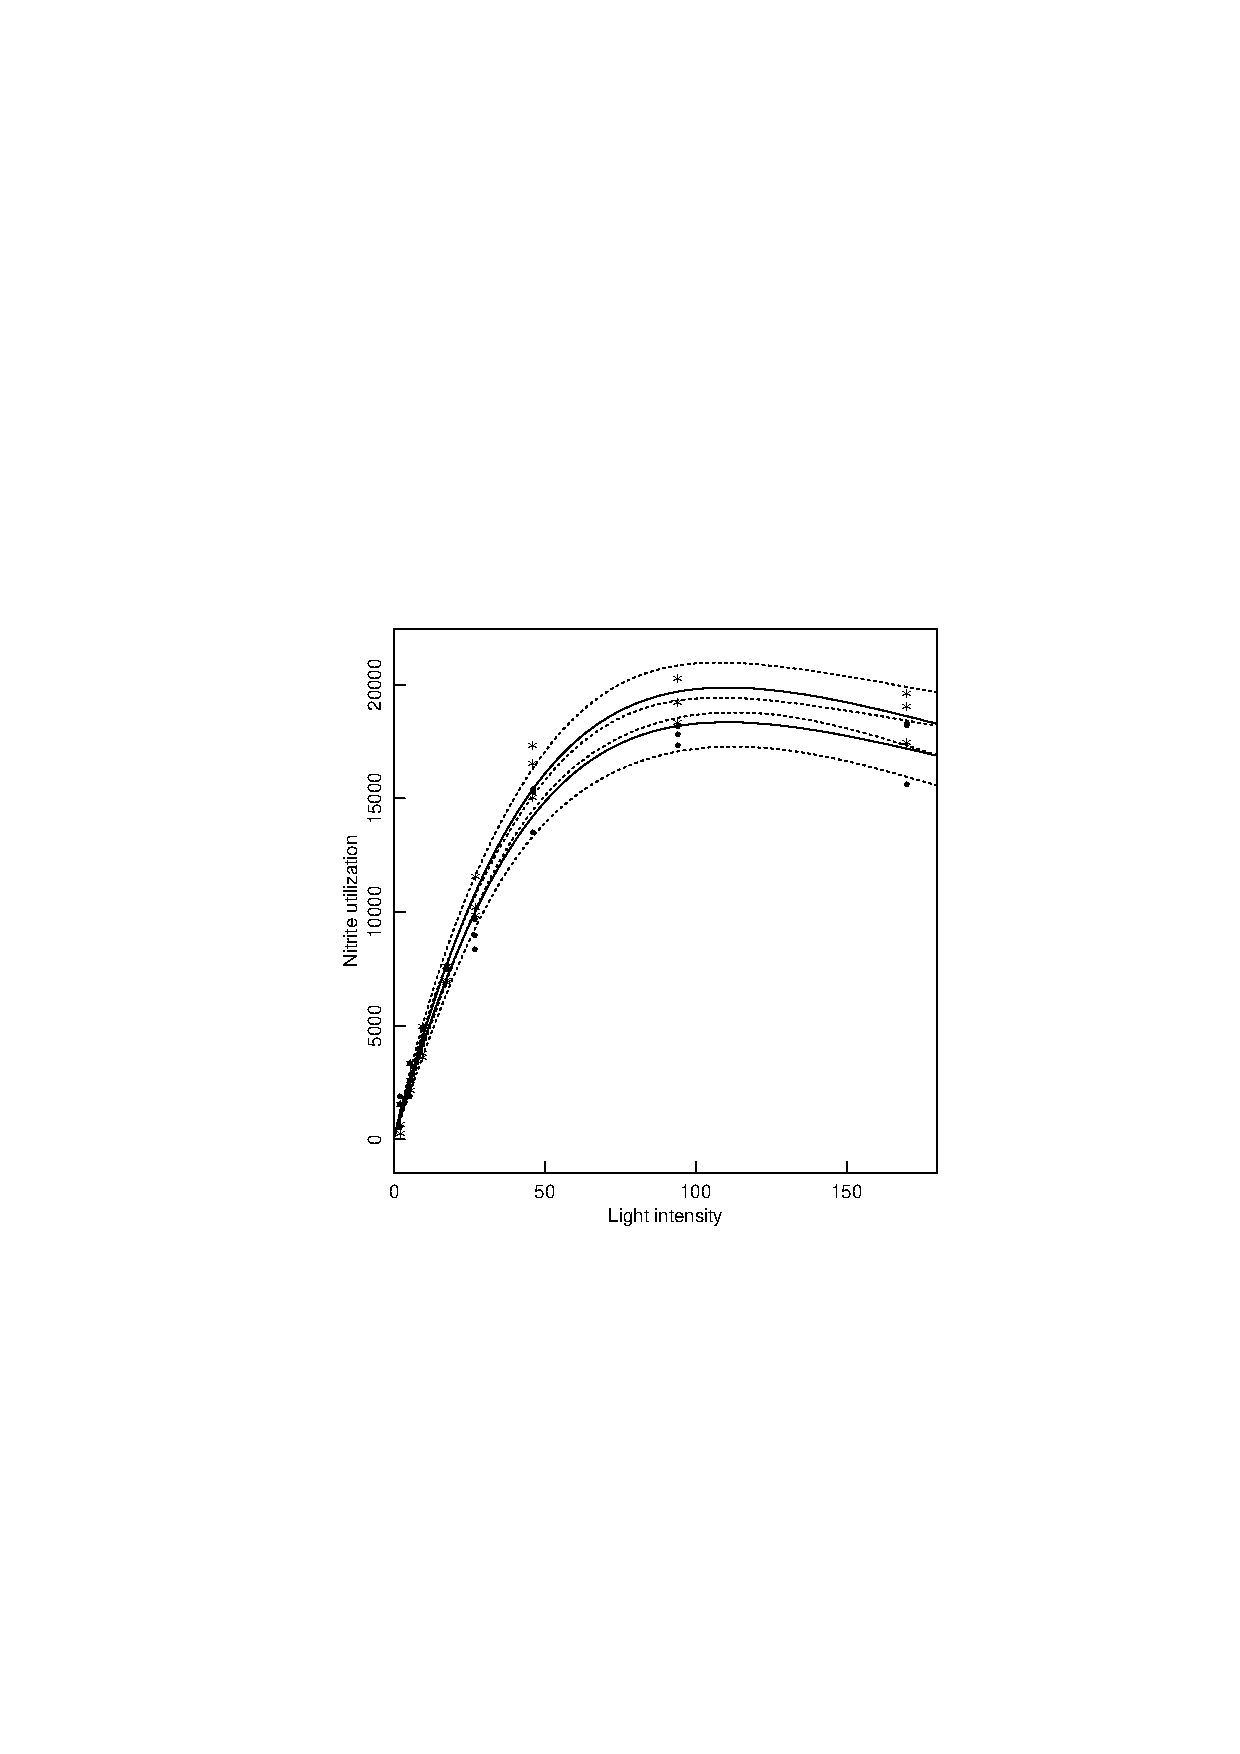
\includegraphics{3NITconfband}}%,height=3in}}
  \caption{Plot of nitrite utilization versus light intensity together
    with the fitted curves (solid lines) and the 95\% approximate
    inference bands (dotted).  Data for day 1 are shown as * and for
    day 2 as .}
  \label{fig:NITconfband}
\end{figure}
we show the nitrite utilization data together with
the fitted curve and the approximate 95\% confidence bands for the
4-parameter quadratic Michaelis--Menten model.

\subsection{Reporting the Results}

A brief report was prepared for Professors Elliott and
Peirson, along the lines of Section 3.12.
The major finding of interest was the need for a model which rose
to a peak rather than to an asymptote.
This was not expected, at least at such a low light level.
As part of our report, we recommended additional experiments be
run, especially at higher light intensities, in order to verify
the need for a model which rises to a peak rather than approaching an
asymptote, and to help discriminate between the two competing models.
It was further suggested that future experiments involve fewer
levels at low light intensity to reduce effort.

\section{Experimental Design}

So far we have concentrated more on the analysis of data
than on the design of experiments to produce good data, although
we believe that good experimental design is vital to
scientific progress.
The reason for the prime importance of experimental design is
that \emph{the information content of the data is established
when the experiment is performed}, and no amount of sensitive data
analysis can recover information which is not present in the
data.

One reason for our emphasizing analysis rather than design is
that we usually have to deal with data that have been
obtained without the benefit of good statistical design.
Another reason is that, while good experimental design is
extremely valuable, it is necessary to know how to analyze data
in order to appreciate what ``good experimental design'' is.

\subsection{General Considerations}
\index{experimental design!general considerations}

Experimentation is fundamental to scientific learning, which we
may characterize as \emph{reducing ignorance}.
At any stage of research, we are in a position of having data,
and of being able to explain part of that data, and
as the research proceeds, we are able to account for, or
explain, more of the data.
For example, a chemical engineer trying to learn about how a
particular product is produced would know very little initially
about the factors and the chemical reactions involved.
As she proceeds, planning and running experiments under various
conditions, she would endeavor to find out, at each stage, what
the important factors are, and how they affect the response.
Initially, she would be involved in empirical ``screening designs''
to try to isolate those factors which are most influential in
affecting the response, probably using \emph{factorial} or
\emph{fractional factorial} designs
\cite{box:hunt:hunt:1978}.
%\glossary{ Box, G.E.P.}
%\glossary{ Hunter, J.S.}
%\glossary{ Hunter, W.G.}
If she was interested in optimizing some characteristic, she
might then proceed to \emph{response surface} designs
\cite{box:drap:1987,box:hunt:hunt:1978}.
%\glossary{ Draper, N.R.}
%\glossary{ Box, G.E.P.}
%\glossary{ Hunter, J.S.}
%\glossary{ Hunter, W.G.}
Later on, perhaps to fine tune the product or to gain better
understanding of the mechanisms involved, she would move from
empirical models and their associated strategies to mechanistic
(usually nonlinear) models.
It is this aspect of experimental design which we consider in
this section.

We assume initially that the experimenter has a well-defined
\emph{form} for the expectation function relating the
factors to the response, and that the objectives
of the experiments are to provide the necessary and adequate
\index{experimental design!objectives}
information to:
estimate the parameters of interest in the model with
  \begin{enumerate}
    \item accuracy (i.e. small bias),\\
          precision (i.e. small variance), and
verify the assumptions about
    \item the expectation function,\\
          the disturbance model.
  \end{enumerate}

As was the case for estimation, it is helpful first to
discuss the linear situation.
Accordingly, in the following section we present a brief review
of experimental design for linear expectation functions.
For a more comprehensive presentation, see
\citeasnoun{box:hunt:hunt:1978},
%\glossary{ Box, G.E.P.}
%\glossary{ Hunter, J.S.}
%\glossary{ Hunter, W.G.}
\citeasnoun{davi:1956}, and \citeasnoun{coch:cox:1957}; and
%\glossary{ Davies, O.L.}
%\glossary{ Cochran, W.G.}
%\glossary{ Cox, G.M.}
for general considerations on the planning of experiments,
\citeasnoun{box:drap:1959} and
%\glossary{ Box, G.E.P.}
%\glossary{ Draper, N.R.}
\citeasnoun{drap:smit:1998}.
%\glossary{ Draper, N.R.}
%\glossary{ Smith, H.}
A thorough review of optimal designs is given in
\citeasnoun{stjo:drap:1975},
%\glossary{ St.John, R.C.}
%\glossary{ Draper, N.R.}
\citeasnoun{coch:1973}, and \citeasnoun{stei:hunt:1984}.
%\glossary{ Cochran, W.G.}
%\glossary{ Steinberg, D.M.}
%\glossary{ Hunter, W.G.}
\citeasnoun{hami:watt:1985} discussed designs using second order
%\glossary{ Hamilton, D.C.}
%\glossary{ Watts, D.G.}
derivatives, and
the geometry of experimental designs was discussed in
\citeasnoun{silv:titt:1973}.
%\glossary{ Silvey, S.D.}
%\glossary{ Titterington, D.M.}

Before considering the more technical details of experimental
design, we offer some comments which help ensure
attainment of the general objectives (1) and (2) above.

With regard to providing accurate and precise estimates of the
parameters, it is helpful to recognize that an experimental
design involves choosing the values of the factors for a selected
number of experimental cases (or runs).
It is therefore important that the number of cases be large
enough to ensure attainment of the specific objectives of the experiment.
For example, if an expectation function involves five
parameters, there will have to be at least five distinct
experimental conditions.
It is equally important to limit the number of experiments done
at any one time.
That is, one should not construct an extremely large design and
then proceed slavishly to follow that design to its completion.
Due account should be taken of what is learned at each stage of
the experiment, and this information should be exploited in the
design of the next stage.
The number of experiments which should be run in a \emph{block}
will depend on the number of factors and the type of experiment
being run, of course, but blocks of size 10 to 20 are usually
informative and manageable.

The choices of the factor settings should be such that they are in
useful and appropriate ranges of the factors.
That is, the factors should be located near sensible
values which will permit use of the parameter estimates in future
investigations, and the levels of each factor should be spread
out enough so that the effect of each factor will be revealed in
spite of the inherent variability of the response.

With regard to
verifying the assumptions about the expectation
function, it is important to provide \emph{replications}
\index{replication}
to enable testing for lack of fit or inadequacy of the
expectation function.
It is also important, when possible, to \emph{randomize}
the order of the
\index{randomization}
experiments, to ensure that the expectation function is appropriate.
(If there are unsuspected factors operating, randomizing will tend
to cause their effects to appear as increased variability rather
than as incorrect parameter estimates, as discussed in Section 1.3.)

With regard to
verifying the assumptions about the disturbance
model, replications are again important.
As discussed in Section 1.3, replications enable one to test for
constancy of variance and to determine a variance stabilizing
transformation if the variance is deemed not constant.
Randomizing will also tend to ensure that all of the
assumptions concerning the disturbances will be appropriate, as
discussed in Section 1.3.
Once again, we see the importance and power of randomizing.

In summary, \emph{statistical analysis} is concerned with the efficient
extraction and presentation of the information embodied in a data set,
while \emph{statistical experimental design}
is concerned first with
ensuring that the important necessary information is embodied in a data
set,
and second with making the extraction and presentation of that
information easy.

\subsection{The Determinant Criterion}
\index{experimental design!for linear expectation functions}

Consider the linear model (1.1)
\begin{displaymath}
\bY=\bX \bbeta+\bZ
\end{displaymath}
with the usual assumptions (1.2) and (1.3) about the disturbances
$\bZ$,
\begin{displaymath}
\mbox{\rm E} [ \bZ ] =  {\bf 0} 
\end{displaymath}
\begin{displaymath}
\mbox{\rm Var} [ \bZ ] = \sigma^2 \bI
\end{displaymath}
For a linear regression model, a row of the derivative matrix $\bX$
depends only on the choice of the $K$ design variables, where the
design variables determine such characteristics as when the run
is taken, at what pressure, at what temperature, etc.
An individual entry in the derivative matrix is calculated from the
values of the design variables.
For any choice of the design variables generating a derivative matrix
\index{derivative matrix}
$\bX$, the parameters
$\bbeta$ will have a joint inference region whose volume
is proportional to $| \bX \trans \bX |^{{-} 1/2}$.
Thus, a logical choice of design criterion is to choose the
design points so that the volume of the joint inference
region is minimized
\index{experimental design!determinant criterion}
\index{experimental design!D-optimal}
\index{D-optimal!design criterion}
\cite{wald:1943}.
%\glossary{ Wald, A.}
Since the power $-1/2$ is inconsequential,
Wald proposed
maximizing the determinant $D = | \bX \trans \bX |$, and
designs which satisfy this criterion are called \emph{D-optimal}
designs.
The criterion is referred to as the \emph{determinant criterion}.
\index{determinant!design criterion}

From a geometric point of view, the determinant criterion implies
\index{geometry!of experimental design determinant criterion}
that we should choose the columns of $\bX$ so that each
vector is as long as possible ($\norm \bx_p \norm^{2}$ is as
large as possible, $p=1 ,2 ,\ldots, P$), and try to make the
vectors orthogonal ($\bx_p \trans \bx_{q=0} ,p!=q$).
The former ensures that the expectation plane will be well supported
in the response space, and that the parameter lines will be widely
spaced on the expectation plane.
Consequently the disturbances, whose variance is beyond our
control, will have small effect, thereby producing a joint region
in the parameter space with small volume.
The latter ensures that the parameter estimates associated with
the factors will not be correlated.
That is, changes in the response will be correctly associated
with changes in the appropriate causative factor, and not
attributed to other factors.

The two requirements of long length and orthogonality
of the derivative vectors
ensure that a disk on the expectation plane will map to a small
ellipse in standard position on the parameter plane.

\index{experimental design!for nonlinear expectation functions}
The determinant criterion was applied to nonlinear expectation
functions by
\citeasnoun{box:luca:1959} who used, in place of the $\bX$
%\glossary{ Box, G.E.P.}
%\glossary{ Lucas, H.L.}
matrix, the derivative matrix $\bV^{0}$ evaluated at
some initial parameter estimates $\btheta^0 $.
That is, in nonlinear design, the $D$-optimal criterion is modified to
maximize
\index{D-optimal!design criterion}
\begin{displaymath}
D = | {\bV^0}\trans\bV^0 |
\end{displaymath}

The design of an experiment depends on the stage at which the
researcher is in an investigation.
When only the form of the model is known, but not the parameter values,
as could be the case in enzyme kinetics or in biochemical oxygen demand
studies, the researcher would be concerned with choosing the values of
the factors to produce good parameter estimates.
These are called ``starting designs.''
Later on in an investigation, the researcher might wish to design an
experiment to improve the precision of estimates of some or all of the
parameters, exploiting data already obtained.
Such designs are called ``sequential designs,''
and, when special interest is attached to a subset of the parameters,
``subset designs.''

\subsection{Starting Designs}
\index{experimental design!starting}

\citeasnoun{box:luca:1959}
%\glossary{ Box, G.E.P.}
%\glossary{ Lucas, H.L.}
proposed starting designs consisting of $P$ points for a
$P$-parameter model, and therefore simplified the criterion
(\ref{eqn:6.1}) to that of maximizing $| \bV^0 |$.
Geometrically, the determinant criterion ensures that the
\index{determinant!design criterion}
expectation surface is such that large regions on the tangent
plane at $\boeta ( \btheta^0 )$ map to small regions
in the parameter space.
When more than $P$ points are to be chosen, the
$D$-optimal design usually results in replications of
$P$ distinct design points \cite{box:1968}, and these design points
%\glossary{ Box, M.J.}
are those that would be chosen as $D$-optimal with $N = P$.
We therefore consider starting designs as having only $P$ runs.

\begin{example}\label{mic:dopt}
To illustrate the choice of a starting design, we consider the case of
enzyme kinetics, which are assumed to follow a Michaelis--Menten model.
We assume that the maximum allowable substrate
concentration is specified as
$x_{max}$, and that initial estimates of the parameters
$\btheta^{0}$ are given.

The derivatives of the expectation function, evaluated at the
initial parameter estimates $\btheta^{0}$, are
\begin{displaymath}
  \frac{x}{\theta_2^0+x}\frac{-\theta_1^0x}{(\theta_2^0+x)^2}
\end{displaymath}
and so the determinant to be maximized is
\begin{eqnarray*}
  | \bV^0 |&=&\left|
  \begin{bmatrix}
    \frac{x_1}{\theta_2^0+x_1}&\frac{-\theta_1^0 x_1}{( \theta_2^0+x_1 )^2}\\
    \frac{x_2}{\theta_2^0+x_2}&\frac{-\theta_1^0 x_2}{( \theta_2^0+x_2)^2}
  \end{bmatrix}\right|\\
  &=&\frac{\theta_1^0 x_1 x_2| x_1-x_2 | }{ ( \theta_2^0+x_1 )^2 (
    \theta_2^0+x_2 )^2}
\end{eqnarray*}
The modulus of this determinant is maximized when
\begin{displaymath}
  x_1=x_{\mbox{\rm max}}\quad\text{and}\quad
  x_2=\frac{\theta_2^0}{1+2(\theta_2^0/x_{\text{max}})}\approx\theta_2^0
\end{displaymath}
The determinant criterion therefore places the design points so
as to tie down the asymptote ($\theta_{1}$) by performing one
experiment at the maximum concentration, and to tie down the
half-concentration by performing the other experiment near the assumed
half-concentration.

It is instructive to compare the $D$-optimal design with the
dilution design used by \citeasnoun{trel:1974}.
%\glossary{ Treloar, M.A.}
The dilution design used $x_{\text{max}}=1.1$ and five dilutions by
approximately one-half, with duplications, giving a total of 12 runs.
With the same number of runs, the $D$-optimal design would consist of 6
replications at $x_{max}$ and 6 replications at
$x_2=\theta_2^0 /[1+2 ( \theta_2^0 / x_{\text{max}})]$.
We take $\theta_2^0  =  0.1$ as a reasonable starting estimate,
and so the design is $x_1  =  1.1$, $x_2  =  0.085$.
In Figure \ref{fig:MICdesign}
\begin{figure}
  \centerline{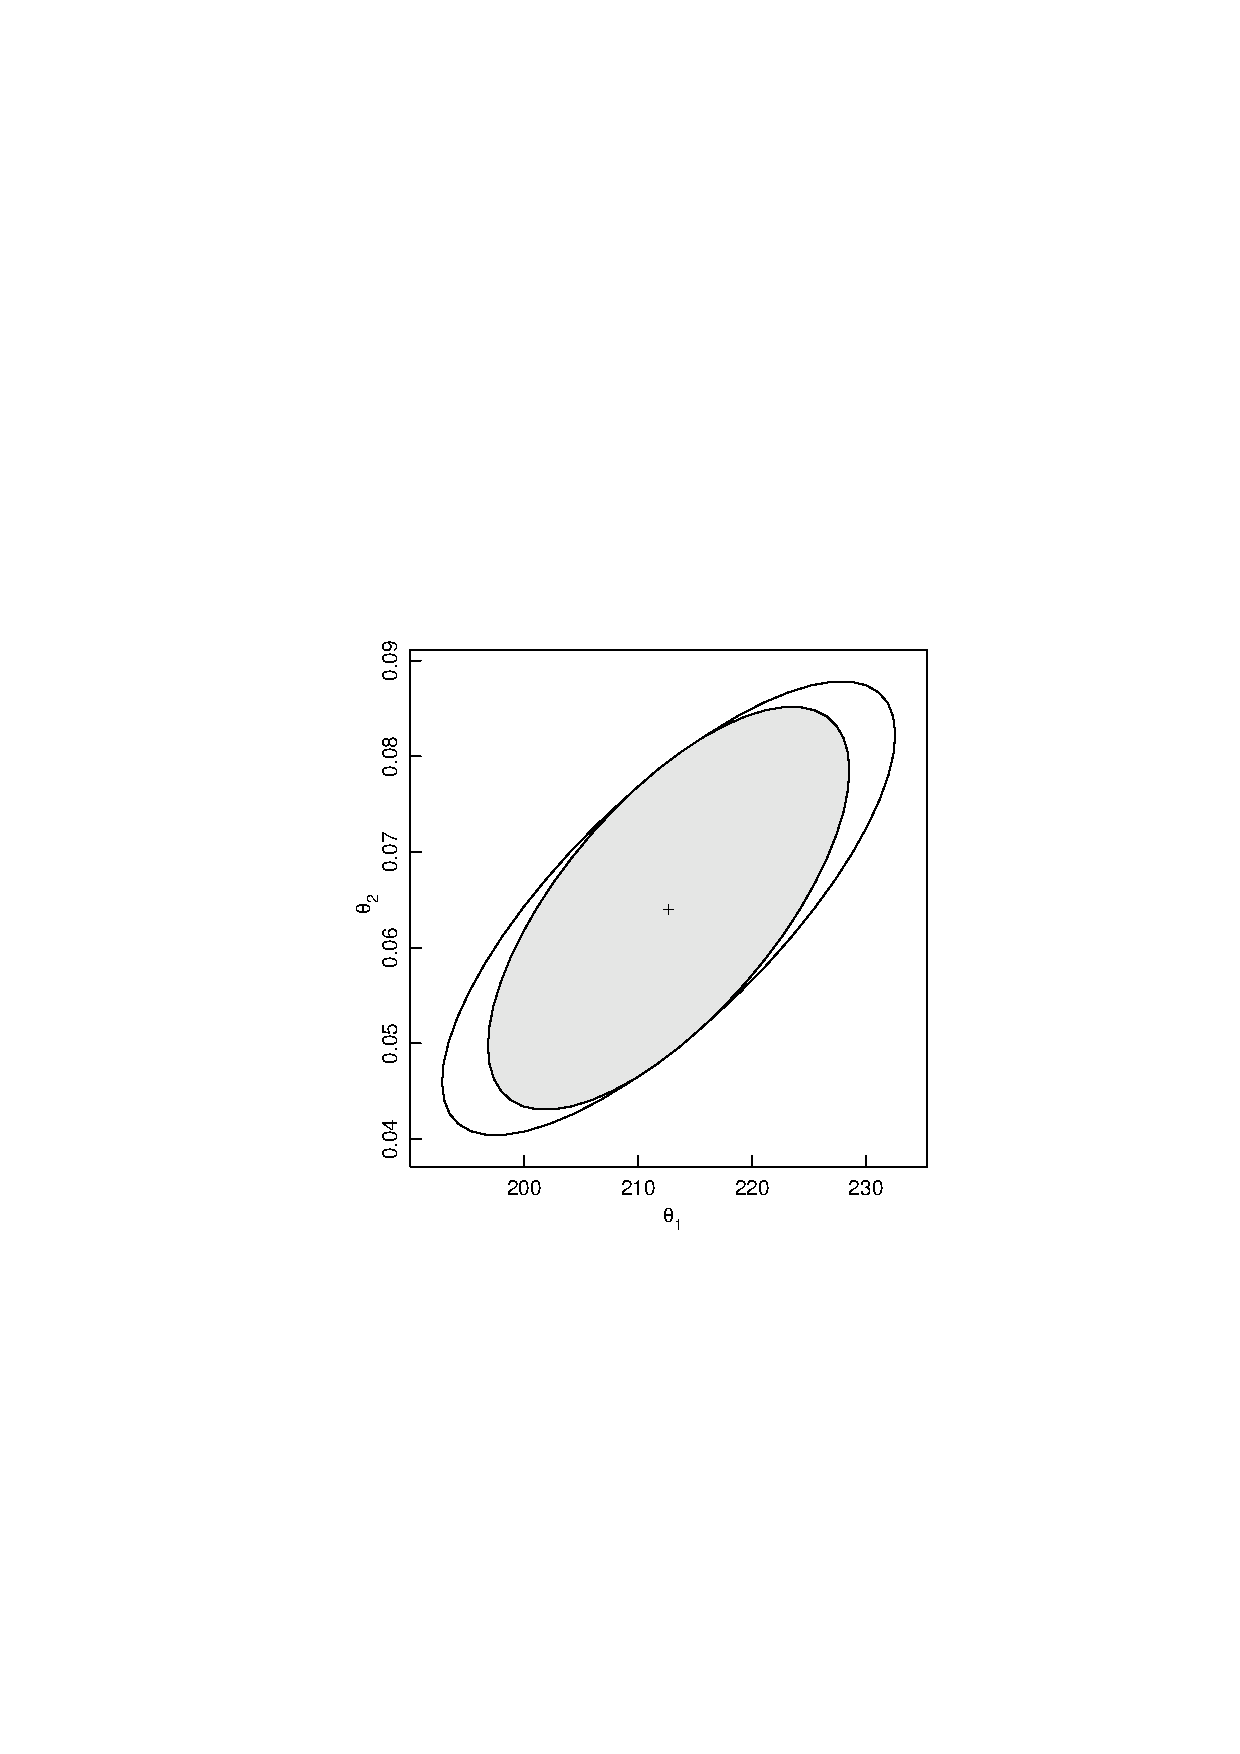
\includegraphics{3MICdesign}}%,height=3in}}
  \caption{Comparison of 95\% approximate inference regions for two
    designs for the Puromycin data.  The larger region results from
    the dilution design used, and the shaded region results from a
    $D$-optimal design.}
  \label{fig:MICdesign}
\end{figure}
we plot the linear approximation 95\% confidence
region for the dilution design and data together with the linear
approximation confidence region for the $D$-optimal design assuming that
both designs gave the same parameter estimates and residual variance.
We see that the $D$-optimal design does indeed give a smaller joint
confidence region and smaller confidence intervals.
In addition, the correlation between the parameters is lower.
However, the gain in precision from using the $D$-optimal design would
have to be balanced against any loss of information about lack of fit.

Note that the design does not depend on the conditionally linear
parameter $\theta_{1}$, which is true in general for conditionally
linear parameters, as shown in Section 3.14.6.
\end{example}

The determinant criterion provides an objective basis for
determining $P$-point designs for $P$-parameter models, but the
design strategy should not be applied blindly.
The criterion was derived on the basis that the expectation
function is \emph{known}, and provides only $P$ design points to
estimate the $P$ parameters.
Replications at these $P$ design points are useful because
\index{replication}
they provide information concerning constancy of
variance, but they cannot provide information about lack of fit.
It might be useful, therefore, to perform additional experiments
at other design points in order to detect lack of fit.
In light of these considerations, the dilution design strategy is
eminently sensible, especially given its high level of performance
as demonstrated in the above example.
\subsection{Sequential Designs}
\index{experimental design!sequential}

In many situations, some experiments will already have been
done to check if the equipment is functioning properly, or to screen
possible models, as described in \citeasnoun{box:hunt:1965}.
%\glossary{ Box, G.E.P.}
%\glossary{ Hunter, W.G.}
In other situations, it may be possible to perform and analyze the
result from a single experiment quite rapidly.
In these situations, it is possible to obtain even better parameter
estimates by designing the experiments sequentially;
that is, an experimental run is designed, the data are collected and
analyzed, and the
design for the next run is obtained by maximizing
$| \bV_1 \trans \bV_1 |$ with respect to the design variables,
$\bx_{N+1}$, where
\begin{displaymath}
\bV_1= \begin{pmatrix}\bV_0\\\bv_{N+1}\end{pmatrix}
\end{displaymath}
and $\bv_{N+1}$ is the gradient vector
$\partial f / \partial \btheta \trans$
evaluated at the least squares estimates from the $N$ runs already made.

\begin{example}\label{iso:dopt}
To illustrate sequential design, we consider the model and data set
from Example Isomerization 1.
The correlations between the parameters are very high, and the linear
approximation confidence regions include negative values for the
equilibrium constants.
We would therefore like to design experiments to provide better
precision in the parameter estimates.

The design points are determined by the values of the partial pressure
of hydrogen, $x_{1}$, the partial pressure of $n$-pentane, $x_{2}$,
and the partial pressure of isopentane, $x_{3}$.
In the previous runs these variables have ranged from about
100 to 400 for $x_{1}$, 75 to 350 for $x_{2}$, and 30 to
150 for $x_{3}$, so we use these limits to define a reasonable
region within which to design further runs.
We begin by evaluating the sequential
$D$-optimal design criterion at the original design points and at
sequential design points at the corners of the region.
This gives the values in Table \ref{tbl:ISOdopt}.
  \begin{table}
\begin{center}
\begin{tabular}{llrc}\hline
 \multicolumn{3}{c}{Factor}  & \multicolumn{1}{c}{Criterion}\\
& & & \multicolumn{1}{c}{$D$}\\
\multicolumn{1}{c}{$x_{1}$} & \multicolumn{1}{c}{$x_{2}$} & \multicolumn{1}{c}{$x_{3}$} & \multicolumn{1}{c}{$10^{6}$} \\ \hline
100&100&30&4.63\\
400&100&30&1.95\\
100&350&30&9.44\\
400&350&30&3.99\\
100&100&150&1.82\\
400&100&150&1.82\\
100&350&150&3.98\\
400&350&150&2.42\\ \hline
\end{tabular}
\end{center}
  \end{table}
The combination which optimizes the $D$-optimal criterion is low
$x_{1}$ (100), high $x_{2}$ (350), and low $x_{3}$ (30).
Examination of nearby values confirms that the
corner is a local optimum, and since a coarse grid search of the
design region did not reveal any optima in the interior,
we choose this corner as the design point for the next run.
\end{example}

\subsection{Subset Designs}
\index{experimental design!subset}

When only a subset of the parameters
$\btheta$ is of interest, the design criterion is modified as suggested
in \citeasnoun{box:1971:biok} and \citeasnoun{hill:hunt:1974}.
%\glossary{ Box, M.J.}
%\glossary{ Hill, W.J.}
%\glossary{ Hunter, W.G.}
We assume that the parameters have been ordered so the first $P_{1}$ 
parameters are the nuisance parameters and the trailing $P_{2}$
parameters are the parameters of interest, and we
partition the vector $\btheta \trans$ as
$( \btheta_1 \trans | \btheta_2 \trans )$
and the matrix $\bV^{0}$ as $[ \bV_1^0| \bV_2^0 ]$.
Then the variance--covariance matrix of the $P_{2}$
parameters is proportional to $\bD_{2,2}$, where
\begin{eqnarray*}
  \bD&=&({\bV^0}\trans \bV^0 )^{-1}\\
  && = \begin{bmatrix}
    {\bV_1^{0}}\trans \bV_1^0 & {\bV_1^{0}}\trans \bV_2^0\\
    {\bV_2^{0}}\trans \bV_1^0 & {\bV_2^{0}}\trans \bV_2^0
  \end{bmatrix}^{-1}\\
  && = \begin{bmatrix}
    \bD_{1,1}& \bD_{1,2}\\
    \bD_{1,2}\trans& \bD_{2,2}
  \end{bmatrix}
\end{eqnarray*}
and so the $D$-optimal criterion is changed to minimization of
\begin{displaymath}
D_S = | \bD_{2,2} |
\end{displaymath}
which is equivalent to maximizing
\begin{displaymath}
\frac{ | { \bV^0 } \trans \bV^0 |}{ | { \bV_1^0 } \trans \bV_1^0 | }
\end{displaymath}

\begin{example}\label{iso:subset}

To illustrate subset design, we consider the model, data set, and
design region from Example Isomerization \ref{iso:dopt}, and treat the
situation in which we wish to improve the estimates of $\theta_{2}$,
$\theta_{3}$, and $\theta_{4}$.
Evaluation of $D_{S}$ at the corners of the same region gives the results
in Table \ref{tbl:ISOsubset},
\begin{table}
  \caption{
  Sequential $D$-optimal subset design criteria for the isomerization model,
  evaluated at the corners of the design region.
  }\label{tbl:ISOsubset}
  \begin{center}
    \begin{tabular}{llrc}\hline
      \multicolumn{3}{c}{Factor}  & \multicolumn{1}{c}{Criterion}\\
      & & & \multicolumn{1}{c}{$D$}\\
      \multicolumn{1}{c}{$x_{1}$} & \multicolumn{1}{c}{$x_{2}$} &
      \multicolumn{1}{c}{$x_{3}$} & \multicolumn{1}{c}{$10^{6}$} \\ \hline
      100&100&30&8.77\\
      400&100&30&3.90\\
      100&350&30&13.11\\
      400&350&30&7.08\\
      100&100&150&3.69\\
      400&100&150&3.68\\
      100&350&150&7.39\\
      400&350&150&4.70\\ \hline
    \end{tabular}
  \end{center}
\end{table}
which produce similar conclusions and the
same design point as in Example Isomerization \ref{iso:dopt}.

\end{example}

\subsection{Conditionally Linear Models}
\index{conditionally linear!model}
\index{experimental design!for conditionally linear model}

It is awkward to have to specify initial estimates of the parameters
$\btheta$ before an experimental design can be obtained, since, after
all, the purpose of the experiment is to determine parameter estimates.
In Examples Puromycin \ref{mic:dopt} and Isomerization \ref{iso:dopt},
we saw that the $D$-optimal design was not affected by the value of a
conditionally linear parameter.
For most models with conditionally linear parameters, the
locations of the $D$-optimal design points do not depend
on the conditionally linear parameters
\cite{hill:1980,khur:1984},
%\glossary{ Hill, P.D.H.}
%\glossary{ Khuri, A.I .}
so the design problem is simpler.

The easiest type of conditionally linear model to demonstrate this for
is that with only one conditionally linear parameter,
so the function can be written
\begin{displaymath}
f ( \bx , \btheta ) = \theta_1  g ( \bx , \btheta_{-1} )
\end{displaymath}
for some function $g$ where
$\btheta_{-1} = ( \theta_2 ,\ldots, \theta_P ) \trans$.
This includes the Michaelis--Menten, BOD, and isomerization models.
The gradient of the model function can then be written
\begin{displaymath}
  \frac{\partial f}{\partial\btheta\trans}=\left(g(\bx,\btheta_{-1}),
    \frac{\partial g}{\partial\btheta_{-1}\trans}\right)
  \begin{bmatrix}
    1 & 0\\
    \bm0 &\theta_1 \bI
  \end{bmatrix}
\end{displaymath}
which isolates the dependence of $\theta_{1}$ from any dependence
upon $\bx$.
Using (\ref{eqn:clfact}), the derivative matrix $\bV$ can be written
\begin{displaymath}
  \bV = \bH ( \bx , \btheta_{-1} )  \bB ( \theta_1 )
\end{displaymath}
where
\begin{displaymath}
\bB ( \theta_1 ) =
\begin{bmatrix}
  1 & 0\\
  \bm0 &\theta_1 \bI
\end{bmatrix}
\end{displaymath}
is $P \times P$, so the $D$-optimal criterion is
\begin{eqnarray*}
  | \bV \trans \bV |&=&| \bB \trans \bH \trans \bH  \bB |\\
  && =  | \bB |^2  | \bH \trans \bH |
\end{eqnarray*}
and, again, the dependence of $\theta_{1}$ is isolated from $\bx$.
Therefore, the design does not depend upon $\theta_{1}$.

In general, for conditionally linear models of the form
\begin{displaymath}
f ( \bx , \btheta ) = \theta_1 g_1 ( \bx , \btheta_{{-} \bL } )
+ \cdots + \theta_L g_L ( \bx , \btheta_{ - \bL } )
\end{displaymath}
where
$\btheta_{ - \bL } = ( \theta_{L+1} ,\ldots, \theta_P ) \trans$,
the
$D$-optimal design will not depend on the conditionally linear parameters
$( \theta_1 ,\ldots, \theta_L ) \trans$ if $\bV$ can be factored as in
(\ref{eqn:dfact}), provided $\bB$ is square.
The condition that the matrix $\bB$ is square was not explicitly stated
in \citeasnoun{hill:1980}, nor was it emphasized in
%\glossary{ Hill, P.D.H.}
\citeasnoun{khur:1984}, where it was shown that
%\glossary{ Khuri, A.I .}
conditionally linear parameters will usually affect subset designs.
This occurs because, for subset designs,
the design criterion involves the \emph{ratio}
of determinants of components of $\bV$, and
so the simple factorization above usually does not occur even if $\bB$ is
square.
\citeasnoun{khur:1984} gives conditions under which
%\glossary{ Khuri, A.I .}
the conditionally linear parameters do not affect designs for
subsets of parameters.

In the common situation where
each component of $\btheta_{-\bL} $ enters into only one of the
functions $g_i ,  i = 1 ,\ldots, L$, the derivatives can be factored
as in (\ref{eqn:dfact}).
For example, $D$-optimal designs for the sum of exponentials model
\begin{displaymath}
f ( x, \btheta ) = \theta_1 e^{ - \theta_2 x } +
\theta_3 e^{ - \theta_4 x } + \cdots +
\theta_{P-1} e^{ - \theta_P x }
\end{displaymath}
do not depend on the conditionally linear parameters.

\subsection{Other Design Criteria}

Precise parameter estimation is not the only objective used for
experimental design.
Methods have been proposed for constructing designs for discriminating
between possible model functions \cite{box:hill:1974} and for balancing
% \glossary{ Box, G.E.P.}
% \glossary{ Hill, W.J.}
the objectives of model discrimination and precise parameter estimation
\cite{hill:hunt:wich:1968}.
% \glossary{ Hill, W.J.}
% \glossary{ Hunter, W.G.}
% \glossary{ Wichern, D.}
The review article \cite{stei:hunt:1984} describes many of these
% \glossary{ Steinberg, D.M.}
% \glossary{ Hunter, W.G.}
criteria.
We also list several of the references for different experimental design
criteria for single response and multiresponse nonlinear models in the
bibliography.

\begin{problems}
  
  \prob Use the data from Appendix 4, Section A4.2 to fit the
  logistic model
  \begin{displaymath}
    f(x,\btheta)=\theta_1+\frac{\theta_2}{1+e^{-\theta_4(x-\theta_3)}}
  \end{displaymath}
  
  \subprob Plot the data versus $x=\log_{10}$ (NIF concentration).
  Note that you will have to make a decision about how to incorporate
  the zero concentration data. You may want to incorporate the actual
  NTD concentrations also.

  
  \subprob Give graphical interpretations of the parameters in the
  model, and use the plot to obtain starting values for each data set.
  
  \subprob Use the starting values in a nonlinear least squares
  routine to find the least squares estimates for the parameters for
  each data set.
  
  \subprob Use incremental parameters and indicator variables to fit
  all of the data sets together.
  
  \subprob Simplify the model by letting some of the parameters be
  common to all of the data sets.  Use extra sum of squares analyses
  to determine a simple adequate model.
  
  \subprob Write a short report about this analysis and your findings.
  
  \prob Use the data from Appendix 1, Section A1.14 to determine an
  appropriate sum of exponentials model.
  
  \subprob Plot the data on semilog paper and use the plot to
  determine the number of exponential terms to fit to the data.
  
  \subprob Use curve peeling to determine starting estimates for the
  parameters.
  
  \subprob Use the starting estimates from part (b) to fit the
  postulated model from part (a).
  
  \prob

  \subprob Use the plot from Problem 2.6 and sketch in the
  curve of steepest descent from the point
  $\btheta^{0}$.
  Hint: The direction of steepest descent is
  perpendicular to the contours.
  \subprob Is the direction of the Gauss--Newton increment
  close to the initial direction of steepest descent?
  \subprob Calculate and plot the Levenberg increment using a
  conditioning factor of $k=4$.
  \subprob Calculate and plot the Marquardt increment using a
  conditioning factor of $k=4$.
  \subprob Comment on the relative directions of the
  Gauss--Newton, Levenberg and Marquardt increment
  vectors.
  
  \prob Use the data from Appendix 4, Section A4.3 to determine an
  appropriate model and to estimate the parameters.
  
  \subprob Plot the concentration versus time on semilog paper,
  and use the plot to determine the number of
  exponential terms necessary to fit the data.
  \subprob Use the plot and the method of curve peeling to
  determine starting values for the parameters.
  \subprob Use a nonlinear estimation routine to estimate the
  parameters.
  
  \prob Use a nonlinear estimation routine and the data and model
  from Appendix 4, Section A4.4 to estimate the parameters.
  Take note of the number of iterations required and any
  difficulties you encounter in each attempt.
  
  \subprob Use any approach you think is appropriate to obtain
  starting values for the parameters in the model.
  \subprob Use your starting values in a nonlinear estimation
  routine to estimate the parameters.
  If you achieve convergence, examine the parameter
  approximate correlation matrix, and comment on the
  conditioning of the model.
  \subprob Reparametrize the model by centering the factor $1/x_3$,
  and use the equivalent starting values from
  part (a) to estimate the parameters.
  If you achieve convergence, examine the parameter
  approximate correlation matrix, and comment on the
  conditioning of the model.
  What effect does this reparametrization have on the
  number of iterations to convergence?
  \subprob Reparametrize the model in part (a) using
  $\theta_{1=e}^{ \phi_1 }$ and $\theta_2=e^{\phi_2}$
  and the equivalent starting values from part (a)
  to estimate the parameters.
  If you achieve convergence, examine the parameter
  approximate correlation matrix, and comment on the
  conditioning of the model.
  What effect does this reparametrization have on the
  number of iterations to convergence?
  \subprob Reparametrize the model in part (b) using the same
  parametrization as in part (c) and the equivalent
  starting values from part (a) to estimate the
  parameters.
  If you achieve convergence, examine the parameter
  approximate correlation matrix, and comment on the
  conditioning of the model.
  What effect does this reparametrization have on the
  number of iterations to convergence?
  
  \prob Use a nonlinear estimation routine and the data and
  model from Appendix 4, Section A4.5 to estimate the
  parameters.
  Take note of the number of iterations required and
  any difficulties you encounter in each attempt.
  
  \subprob Use any approach you think is appropriate to obtain
  starting values for the parameters in the model.
  \subprob Use your starting values in a nonlinear estimation
  routine to estimate the parameters.
  If you achieve convergence, examine the parameter
  approximate correlation matrix, and comment on the
  conditioning of the model.
  \subprob Reparametrize the model in part (a) using $\theta_2
  e^{ - \theta_3 x }= e^{ - \phi_3 ( x - \phi_2 ) }$.
  If you achieve convergence, examine the parameter
  approximate correlation matrix, and comment on the
  conditioning of the model.
  What effect does this reparametrization have on the
  number of iterations to convergence?
  
  \prob 
  
  \subprob Show that the theoretical $D$-optimal starting
  design for the logistic model of Problem 3.1
  consists of $\bx=(-\infty,\theta_3-1.044/
  \theta_4,\theta_3+1.044/ \theta_4,+\infty)\trans$. 
  \subprob Interpret the choice of the design points
  graphically by plotting the logistic function versus
  $x$ and plotting the location of the design points
  on the $x$-axis.
  \subprob Plot the derivatives with respect to the parameters
  versus $x$ and use these plots to help interpret the
  choice of the design points.
  
\end{problems}

% Local Variables: 
% mode: latex
% TeX-master: "nraia2"
% End: 
